\documentclass[12pt,letterpaper]{article}

\PassOptionsToPackage{hyphens}{url}


\usepackage{setspace}
\onehalfspacing

% === MARGINS ===
\addtolength{\hoffset}{-0.75in} 
\addtolength{\voffset}{-1.25in}
\addtolength{\textwidth}{1.5in} 
\addtolength{\textheight}{2.25in}

% == ENVS ==
\newenvironment{tightcenter}{%
  \setlength\topsep{0pt}
  \setlength\parskip{0pt}
  \begin{center}
}{
  \end{center}
}

% == PACKS ==
\usepackage{color,soul}
\usepackage{graphicx} % to use pngs in tex (include graphix)
\usepackage{calc} % To scale \pagewidth with \real{float}
\usepackage{pgfplots} % To draw histogram

\pgfplotsset{
  compat=1.17, 
colormap/viridis
} % request specific version of pgfplots
\usepackage{calc} % to use \real for text -> numeric
\usepackage{pgf} % to store numeric variables
\usepackage{subcaption} % to place two figures horizontally
\usepackage{caption} % to refer subfigure
\renewcommand{\thesubfigure}{(\alph{subfigure})}
\captionsetup[sub]{labelformat=simple}
\captionsetup[table]{font={stretch=1.2}}  % adjust line space in captions of TABLE and FIGURES
\captionsetup[figure]{font={stretch=1.2}}  


\usepackage{tikz}
\usetikzlibrary{automata,positioning}
\usetikzlibrary{arrows.meta, positioning, automata}
\usetikzlibrary{spy}
\usetikzlibrary{shadows}

\tikzset{
  font={\fontsize{10pt}{0}\selectfont}}
\usepackage{forest}
\tikzset{
  Decision/.style = {%
    draw,
    line width=1.4pt
  },
  Lottery/.style = {%
    draw,
    line width=1.4pt
  },
  Outcome/.style = {%
    circle,
    minimum width=3pt,
    fill,
    inner sep=0pt
  }
}
\usepackage{csquotes}
\usepackage{lipsum}
\usetikzlibrary{arrows.meta,automata,positioning} % to draw directed-weighted-graph


\usepackage{amsmath, amssymb, latexsym} % NN
\usepackage{tikz}% NN
\usetikzlibrary{decorations.pathreplacing}% NN
\usetikzlibrary{fadings}% NN


\usepackage{xltabular}
\usepackage{booktabs}

\usepackage[breakable, skins]{tcolorbox} % to add factual asepct inside a frame

\usepackage[title]{appendix}

%to prevent page and footnotes swalloen by the table


% == Checkmarks == 
\usepackage{bbding}
\usepackage{pifont}
\usepackage{wasysym}
\usepackage{amssymb}
% ================

% == BIBS ==
\usepackage{natbib}

\usepackage{diagbox}

\usepackage[bottom]{footmisc}

\usepackage[
  hidelinks,
  pdftex, 
  bookmarksopen=true, 
  bookmarksnumbered=true,
  pdfstartview=FitH, 
  breaklinks=true, 
  urlbordercolor={0 1 0}, 
  citebordercolor={0 0 1}]
  {hyperref}

\usepackage[ruled,vlined]{algorithm2e}
\SetKwFor{For}{for (}{) $\lbrace$}{$\rbrace$}

%%% Coloring the comment as blue
\newcommand\mycommfont[1]{\footnotesize\ttfamily\textcolor{blue}{#1}}
\SetCommentSty{mycommfont}

\SetKwInput{KwInput}{Input}                % Set the Input
\SetKwInput{KwOutput}{Output}   
\usepackage{algpseudocode}% http://ctan.org/pkg/algorithmicx
\usepackage{varwidth}% http://ctan.org/pkg/varwidth

\bibliographystyle{apsr}

% == SPACES == 

% == CMMDS ==
\newcommand{\tit}{
\bf 
Mapping Regulatory System of WTO Dispute Settlement Body Using Deep Learning
% Mapping Network of Articles of WTO Agreements Using Deep Learning
}
\newcommand\spacingset[1]{\renewcommand{\baselinestretch}
{#1}\small\normalsize}

% To draw embedding layer
\newcommand*{\xMin}{0}%
\newcommand*{\xMax}{6}%
\newcommand*{\yMin}{0}%
\newcommand*{\yMax}{9}%
% To draw conv output
\newcommand*{\xMinOut}{10}%
\newcommand*{\xMaxOut}{11}%
\newcommand*{\yMinOut}{1}%
\newcommand*{\yMaxOut}{8}%


% == VARS == 
\pgfmathsetmacro{\heatmap}{1}

% == START (PageCounter, Mode)
\begin{document}

\spacingset{1.25}

\setcounter{page}{0}
\vspace{-.1in}

% == TITLE (includes DraftDate)
{\title{
    \tit
  }
  \author{Suyeol Yun
  }
  \maketitle
}

\thispagestyle{empty}
\vspace{-.1in}

\begin{abstract}
  % \lipsum[1]
\end{abstract}

\spacingset{1.5} % gives a slightly more margin between abstract and introduction

% \section{Tree of Contents}
% \begin{forest}
  for tree={
  % grow=-1,
  Decision,
  }
  [Introduction
    [How WTO works]
    [Complexity in Legal Citation
        [Origin of Complexity
            [Strategic Consideration]
        ]
        [Importance of Understanding this Complexity
          [Difficult to Map this Complexity]
        ]
    ]
  ]
\end{forest}

% \clearpage

% == INTRO ==
\section{Introduction}

The Dispute Settlement Body (DSB) of 
the World Trade Organization (WTO) deals 
with trade disputes between WTO members.
WTO members can file a lawsuit in WTO DSB to 
claim their impaired benifit related to the WTO agreements as a result of possible illegal action of the other member's trade policy.
Then a judicial body, \textit{Panel} or \textit{Appellate Body}, %``Panel'' or ``Appellate Body'', 
adjudicates the dispute and submits a report in which it expresses
its judicial opinion as to whether the challenged 
trade policy is inconsistent to the rules of the WTO or not \citep{world2017handbook}.

 
% References
% https://www.wto.org/english/tratop_e/dispu_e/disp_settlement_cbt_e/c3s3p1_e.htm


A lawsuit tends to cite multiple rules of the WTO agreement because a trade policy is usually pretty much complicated
and one simple rule can't cover the characteristics of the trade policy at issue \citep{palmeter2004dispute}.
For example, the United States enacted \textit{Continued Dumping and Subsidy Act of 2000 (Byrd Amendment)} that distributes
the collected anti-dumping duties to its affected domestic producers and this act was challenged with multiple rules of the WTO agreement,
such as \textit{Anti-dumping} and \textit{Subsidy}, because
this distribution could constitute a illegal subsidy prohibited
in the rules of the WTO agreement although it's mainly related to the rules of the anti-dumping \citep{cdsoa}.
 
% Todos:
% - How to cite us laws? Byrd amendment


Moreover, legal citation becomes even more complicated because members cite the 
rules of the WTO agreement strategically. For example,
members cite different rules of the WTO agreement to limit or to encourage 
the third party participation because the third party 
participation can lead to eary settlement of the dispute without continuos 
legal battle and vice versa  \cite{who_gets}.
As WTO sets multiple principles to regulate the world trade system, 
such as \textit{Market Acceess} (across borders), 
\textit{Non-discrimination} (between members 
or between domestic products and imported products) 
and \textit{Transparency} (in publication and maintaining 
of each member's internal regulations), 
it's intellectually intriguing 
to understand how regulatory system of WTO DSB
is structured to achieve these core principles.
By understanding this structure, 
we can improve WTO system more efficiently to adopt to constantly 
changing circumstances of world trade
\citep{FREDEBEULKREIN1999625, shaffer_2004, 10.1093/jiel/jgm028}.




However, it is extremely difficult to 
visually map how regulatory power of 
WTO DSB is organized to acheive 
those core principles. 
As explained above, 
this is because each citation is closely related 
to composite characteristics 
of each trade policy and also 
it requires to generalize those strategic 
citations which are limited 
to each member's special interest 
rather than explaining the 
regulatory power of WTO DSB in general. 


\begin{figure}[ht]
    \[\text{Network of legal articles of WTO agreements is defined as}\] %\textit{directed weighted graph}}  G = (V, E, w) \]
    \[ \textit{directed weighted graph }G = (V, E, W) \]
    \[\text{ where \textit{vertex set} } V = \{v \mid v\text{ is a legal article of WTO agreement}\}  \text{ , } \]
    \[\text{ \textit{set of directed edges }}\vec{E} = \{(v_i, v_j) \mid (v_i, v_j)\in V \times V)\} \text{ and } \]
    \[w : V \times V \to \Bbb R_{+} \text{ } s.t. \text{ } w(v_j, v_j) = 0 \text{ and } \sum_{v_i\in V}{w(v_i, v_j)} = 1 \text{  } \forall v_j \in V \]%\text{ and }\]
    \[\text{Then define \textit{edge weight matrix }}W=(w_{ij}) \in \Bbb{R_{+}}^{|V| \times |V|} \text{ } s.t. \text{ } w_{ij} = w(v_i, v_j) \] % \text{ } s.t. \text{ } w_{ii} = 0 \text{ and } \sum_{v_j\in V}{w_{ji}} = 1 \text{  } \forall v_i \in V \] %\text{ } s.t. \text{ } w_{ij} = w(v_i, v_j)\]
    % \[w_{ij} \text{ notates the weight of a directed edge from } v_i \text{ to } v_j \text{ and }  \]
    \[(W \text{ is more formally called \textit{weighted adjancency matrix}})\]
    % \[w_{ij} \text{ represents a directed edge weight from source node $v_i$ to $v_j$} \text{ and }\]
    % \[w_{ij} \text{ is interpreted as conditional probability P(v_j|v_i)}\]
    % \[\text{ where a source node $v_i$ clarifies the meaning of the target node $v_j$}\]
    % \[w : V \times V \to \Bbb R_{+} \text{ } s.t. \text{ } w(v_i, v_i) = 0 \text{ and } \sum_{v_j\in V}{w(v_i, v_j)} = 1 \text{  } \forall v_i \in V \]%\text{ and }\]
    % \[\text{ Then define \textit{edge weight matrix} } W=(w_{ij}) \in \Bbb{R}^{|V| \times |V|} \text{ } s.t. \text{ } w_{ij} = w(v_i, v_j)\]
    % \[\text{ This paper assumes there exists } W^{*}=(w^{*}_{ij}) \in \Bbb{R}^{|V| \times |V|} \text{ } s.t. \text{ } w_{ij} = w(v_i, v_j)\]
    % \[\text{(}G\text{ is simply called \textit{directed weighted graph)}}\]
    \caption{\textbf{Formal Definition of Network of Legal Articles of WTO agreements: }I define network of legal articles of WTO agreements
        as a directed weighted graph where the sum of all weights coming into a node sum up to 1. $w_{ij}$ is interpreted as conditional probability $P(v_j|v_i)$ how probably a source node $v_i$ clarifies the meaning of the target node $v_j$ compared to other source nodes as illustrated in Figure \ref{fig:def-example}}
    \label{fig:def}
\end{figure}

% % == DEF EXAMPLE == 
\begin{figure}[]
    \captionsetup[subfigure]{justification=centering}
    \begin{subfigure}[b]{1\textwidth}
        \centering{
                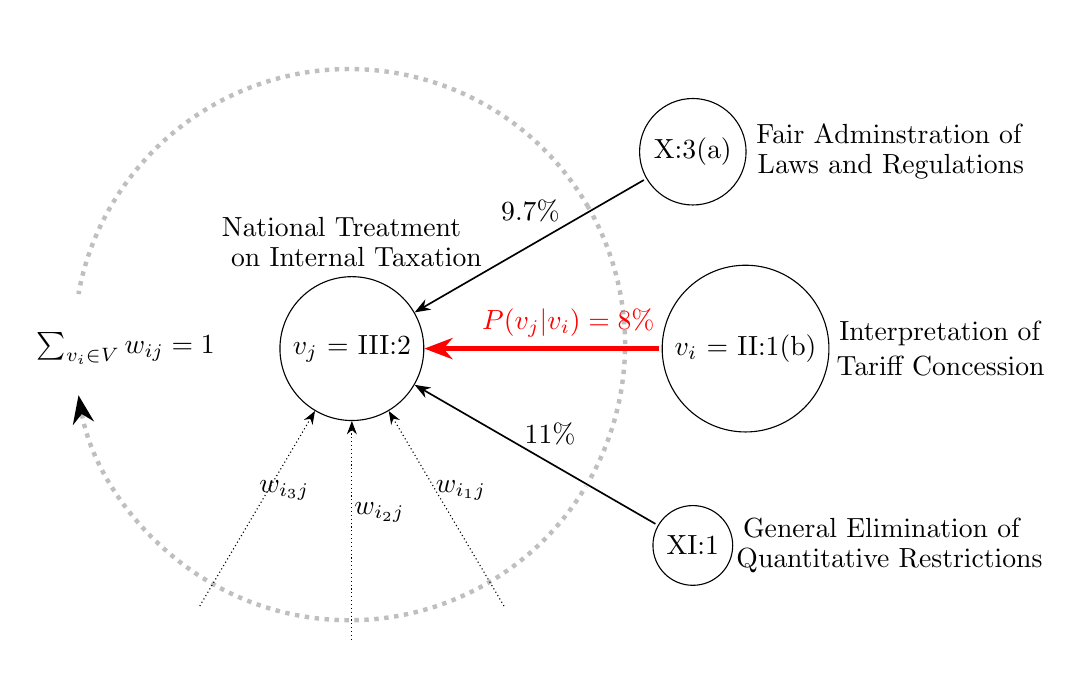
\begin{tikzpicture}[
        >={Stealth[color=black]}
        ,shorten >=1pt,node distance=2cm
        ,on grid,initial/.style={}
        ,every label/.style={align=left}
        ]
        \linespread{2}
        \node[state, label=above:{National Treatment \\[1mm] \hspace{0mm} on Internal Taxation}] (T1) at (10, 0) {$v_j$ = III:2};

        \node[text width=5cm] at (8.5,0)
        {$\sum_{v_i\in V}{w_{ij}} = 1$};

        \draw[ultra thick, gray!50, dotted, ->] (13,1.8) arc (30:-170:3.5);
        \draw[ultra thick, gray!50, dotted, -] (13,1.8) arc (30:170:3.5);

        \node[state, label=right:{Interpretation of \\[1mm] \hspace{-1.5mm} Tariff Concession}] at ([shift=({0:5 cm})]T1) (T2) {$v_i$ = II:1(b)};
        \node[state, label=right:{General Elimination of \\[1mm] \hspace{-2mm} Quantitative Restrictions}] at ([shift=({-30:5 cm})]T1) (T3) {XI:1};
        \node[state, label=right:{Fair Adminstration of \\[1mm] \hspace{-1mm} Laws and Regulations}] at ([shift=({30:5 cm})]T1) (T4) {X:3(a)};
        
        \draw[red,arrows={[red]<-}, ultra thick] node[above, xshift=12.75cm] {$P(v_j|v_i) = 8\%$} (T1) -- (T2);

        \begin{scope}[every edge/.append style={<-}] % for directed edge, change "style={->, double=black, draw=white}]"
            \path
            % (T1) edge[red, ultra thick] node[above] {$0.092$} (T2)
            (T1) edge[double=black, draw=white] node[above, xshift=5pt] {$11\%$} (T3)
            (T1) edge[double=black, draw=white] node[above, yshift=5pt] {$9.7\%$} (T4);

            \path[->] (T1) edge[thin,<-,densely dotted] node[above, xshift=5pt] {$w_{i_{1}j}$} +(1.95,-3.3);
            \path[->] (T1) edge[thin,<-,densely dotted] node[above, xshift=10pt] {$w_{i_{2}j}$} +(0,-3.75);
            \path[->] (T1) edge[thin,<-,densely dotted] node[above, xshift=10pt] {$w_{i_{3}j}$} +(-1.95,-3.3);
        \end{scope}

    \end{tikzpicture}

% \begin{figure}[ht]
%     \centering
    
%     \caption{\textbf{Example of Network of Legal Articles of WTO agreements: }}
%     \label{fig:def-example}
% \end{figure}

        }
        \caption{\textbf{Illustrated edge weights of a target node Article III:2}}
        \label{subfig:a:art2b}
    \end{subfigure}
    \vfill
    \begin{subfigure}[b]{1\textwidth}
        \centering{
            \begin{displayquote}[][]
    \begin{center}
    \end{center}
  
    \begin{displayquote}[][]
    ``The dictionary definition of the noun `excess' is `[t]he amount by which one number
        or quantity exceeds another'. More specifically, `in excess of' means `more than'. Thus,
        as a textual matter, a particular number or quantity is `in excess of' another number
        or quantity if it is greater, regardless of the extent to which it is greater. 
      \textbf{\textit{Looking at the context of Article II:1(b), first sentence, we note that Article III:2, first
      sentence, of the GATT 1994 is cast in very similar terms and in fact uses the phrase
      `in excess of'}}:\\
        \begin{displayquote}
        The products of the territory of any contracting party imported into the
      territory of any other contracting party shall not be subject … to internal
      taxes or other internal charges of any kind in excess of those applied … to
      like domestic products \ldots
        \end{displayquote}   
    \end{displayquote}  
  \end{displayquote}

        }
        \centering
        \caption{\textbf{Jurisprudence of Panel in \textit{Russia – Tariff Treatment} case:} \\ Panel clarifies the point that the meaning of the term \textit{`in excess of'} in Article II:1(b) \\ clarifies the meaning of the same phrase in Article III:2.}
        \label{subfig:a:condprob}
    \end{subfigure}
    \caption{\textbf{Illustration of Network of Legal Articles of WTO agreements: }Every directed edge weight $w_{ij}$ is interpreted as the conditional probability $P(v_j|v_i)$ of how probably a source node $v_i$ constitutes a legal context to clarify the meaning of the target node $v_j$ among all other source nodes $v\in V \setminus \{v_i, v_{j}\}$. Above subfigure (a) represents how jurisprudence of \textit{Panel} stated in (b) is represented as an edge weight where the source node Article II:1(b) constitutes the legal context of the target node Article III:2 regarding how to interpret its term \textit{`in exccess of'} with the $8\%$ of importance compared to other possible source articles.}
    \label{fig:def-example}
\end{figure}

\begin{displayquote}[][]
  \begin{center}
    Article 7\\
    Terms of Reference of Panels
  \end{center}

  1. Panels shall have the following terms of reference unless the parties to the dispute
  agree otherwise within 20 days from the establishment of the panel:

  \begin{displayquote}[][]

    ``To examine, in the light of {\bf the relevant provisions} in (name of the covered
    agreement(s) cited by the parties to the dispute), the matter referred to the DSB by
    (name of party) in document … and to make such findings as will assist the DSB in
    making the recommendations or in giving the rulings provided for in that/those
    agreement(s).''
      
  \end{displayquote}

  2. Panels shall address {\bf the relevant provisions} in any covered agreement or agreements
  cited by the parties to the dispute.

  \ldots
\end{displayquote}


\begin{figure}[]
    \begin{center}
        Article I
    \end{center}
    \begin{center}
        \textit{General Most-Favoured-Nation Treatment}
    \end{center}
    1. With respect to customs duties and charges of any kind imposed on or in connection
    with importation or exportation or imposed on the international transfer of payments for
    imports or exports, and with respect to the method of levying such duties and charges, and
    with respect to all rules and formalities in connection with importation and exportation, and
    with respect to all matters referred to in paragraphs 2 and 4 of Article III, any advantage,
    favour, privilege or immunity granted by any contracting party to any product originating in
    or destined for any other country shall be accorded immediately and unconditionally to the
    like product originating in or destined for the territories of all other contracting parties...
    \caption{\textbf{Example of a legal article of the WTO agreements:} Article I:1 of General Agreement on Tariffs and Trade 1994 that prohibits the discrimination between members of WTO.}
    \label{fig:gatt_art1}
\end{figure}


To train this neural network, this paper collected textual description of trade policy 
that led to the dispute and articles of the WTO agreement cited for each dispute
case requested to the WTO DSB 
from 1995 to 2018 (\hyperref[sub:cited-articles-table]{Total $143$ cases. \textit{Check} the list in Appendix A.2}).
Using this collected data, I trained the neural network by enforcing the neural network to answer correctly 
whether a given article of the WTO agreements
can be cited for the given textual description of 
trade policy that led to the dispute (\textit{See} Figure \ref{fig:design-of-nn} and Figure \ref{fig:def:io:nn}).
% After finish training, I collected all the predictions from the trained neural network (Figure \ref{predidction_matrix})
% and fitted a best network of legal articles of the WTO agreement
% using this collection of answers.
After training, I fitted a set of directed edge weight $W^*$ that 
best explains the variance of each article's citability predicted by the trained deep neural network using a ensemble of random forests \citep{genie3}. 

%for given $V$, $E$ % and collection of answers from the trained neural network (Figure \ref{predidction_matrix}) 
%which is widely used in the biomedical engineering to reconstruct gene regulatory networks.\footnote{Anaology of international normative system to genetics maybe natural because gene expressions (achieving main principles of WTO) are governed by complex interaction between multiple regulatory proteins (interaction between legal articles of WTO). Similar notion is adopted in \cite{gene_analogy} to explain the the evolution of norm of transparency in international security.}

To check whether this fitted network of articles of the WTO agreements $G^*$ = ($V$, $E$, $W^*$) maps the regulatory system of WTO DSB properly, this paper
compares the fitted network $G^*$ with the jurisprudence of WTO DSB made by \textit{Panel} and \textit{Appellate Body}. 
This comparison reveals that the fitted network $G^*$ captures the interaction between the articles of WTO agreements
similarly with the jurisprudence of \textit{Panel} and \textit{the Appellate Body}. This similarity guarantees that the fitted network $G^*$ closely maps the regulatory system of WTO DSB since only these two judicial bodies 
can authoritatively consitute the jurisprudence over how rules of WTO agreements are working together 
to achieve the main principles of WTO.

% Morover, this paper justifies the use of textual information inside the textual description of the dispute and legal article by showing that simply using the co-citation pattern between articles of the WTO disputes can't qualitatively fit the $G^*$ (\textit{See} Figure \ref{fig:adj} and Figure \ref{}). 
% Upon this necessity of using the textual information, this paper also justifies the use of neural network that is computationally intensive since it's generally known that proper design of neural network is able to effectively extract information from the textual content.

% Finally, I will explain how this fitting of network of legal articles can contribute to the current study of international normative system.

% \begin{itemize}
%     \item It shows that the result neural network well match with the result of main two judicial bodies.
% \end{itemize}


% == DATA ==
\section{Data: Types, Composition and Collection Process} \label{sec:data}
This section explains the composition of data 
and its collection process in detail. 


\subsection{Overview: How Members Raise Claims in WTO DSB}
As explained in the introduction,
a trade policy that led to a dispute (preferably called as \textit{Government Measure} in WTO DSB) is pretty much complicated as explicitly expressed by the Panel in Figure \ref{fig:complex-measure}.
To address this complexity,
members who raise the claim (preferably called \textit{complainant} in WTO DSB) usually cite multiple articles of the WTO agreements at the same time. For example, in the
\textit{US - Offset} case,
a group of complainants\footnote{Australia,
   Brazil,
   Chile,
   European Communities,
   India,
   Indonesia,
   Japan,
   Korea and Thailand}
cited articles as shown in Table \ref{xltabular:cited-article-for-us-offset} from the WTO agreements to claim its inconsistencies of \textit{Continued Dumping and Subsidy Act of 2000} (CDSOA) to those cited articles\footnote{It is worth noting that the WTO agreements comprises many different agreements covering each specific topic in trade such as \textit{Agreement on Anti-dumping, Agreement on Subsidies and Countervailing Measures, Agreement on Agriculture} and so on.}:
\\
\begin{table}[h]
   \setlength\tabcolsep{15pt}
   \begin{tabular}{ c | c }
       \hline
       \textbf{\normalsize Name of WTO Agreement}          & \textbf{\normalsize Cited Articles} \\
       \hline \hline
       Agreement on Anti-dumping                           & 1, 5.4, 8, 18.1, 18.4               \\ \hline
       General Agreement on Tariffs and Trade 1994         & VI:3, X:3, XXIII:1, VI:2            \\ \hline
       Agreement on Subsidies and Countervailing Measures  & 4.10, 7.9, 10, 11.4, 18, 32.1, 32.5 \\ \hline
       Agreement Establishing the World Trade Organization & XVI:4                               \\ \hline
   \end{tabular}
   \caption{Cited articles in \textit{US - Offset (Byrd Amendment)} by complainants}
   \label{xltabular:cited-article-for-us-offset}
\end{table}
 
\noindent Upon this understanding,
I collected two different types of data for 143 different dispute cases requested to WTO DSB. (List of cases is
available at \hyperref[sub:cited-articles-table]{Appendix A.2}).
One is textual description of the dispute \hyperref[sub:factual-aspect-example]{(\textit{Check} the CDSOA example at Appendix A.1)} and the other one is
set of articles of the WTO agreements that are
cited for each dispute \hyperref[sub:cited-articles-table]{(Appendix A.3)}.
I will explain the data source, structure and collection method for two different types of data at the following subsections.\\
 
\begin{figure}[h]
    \centering
    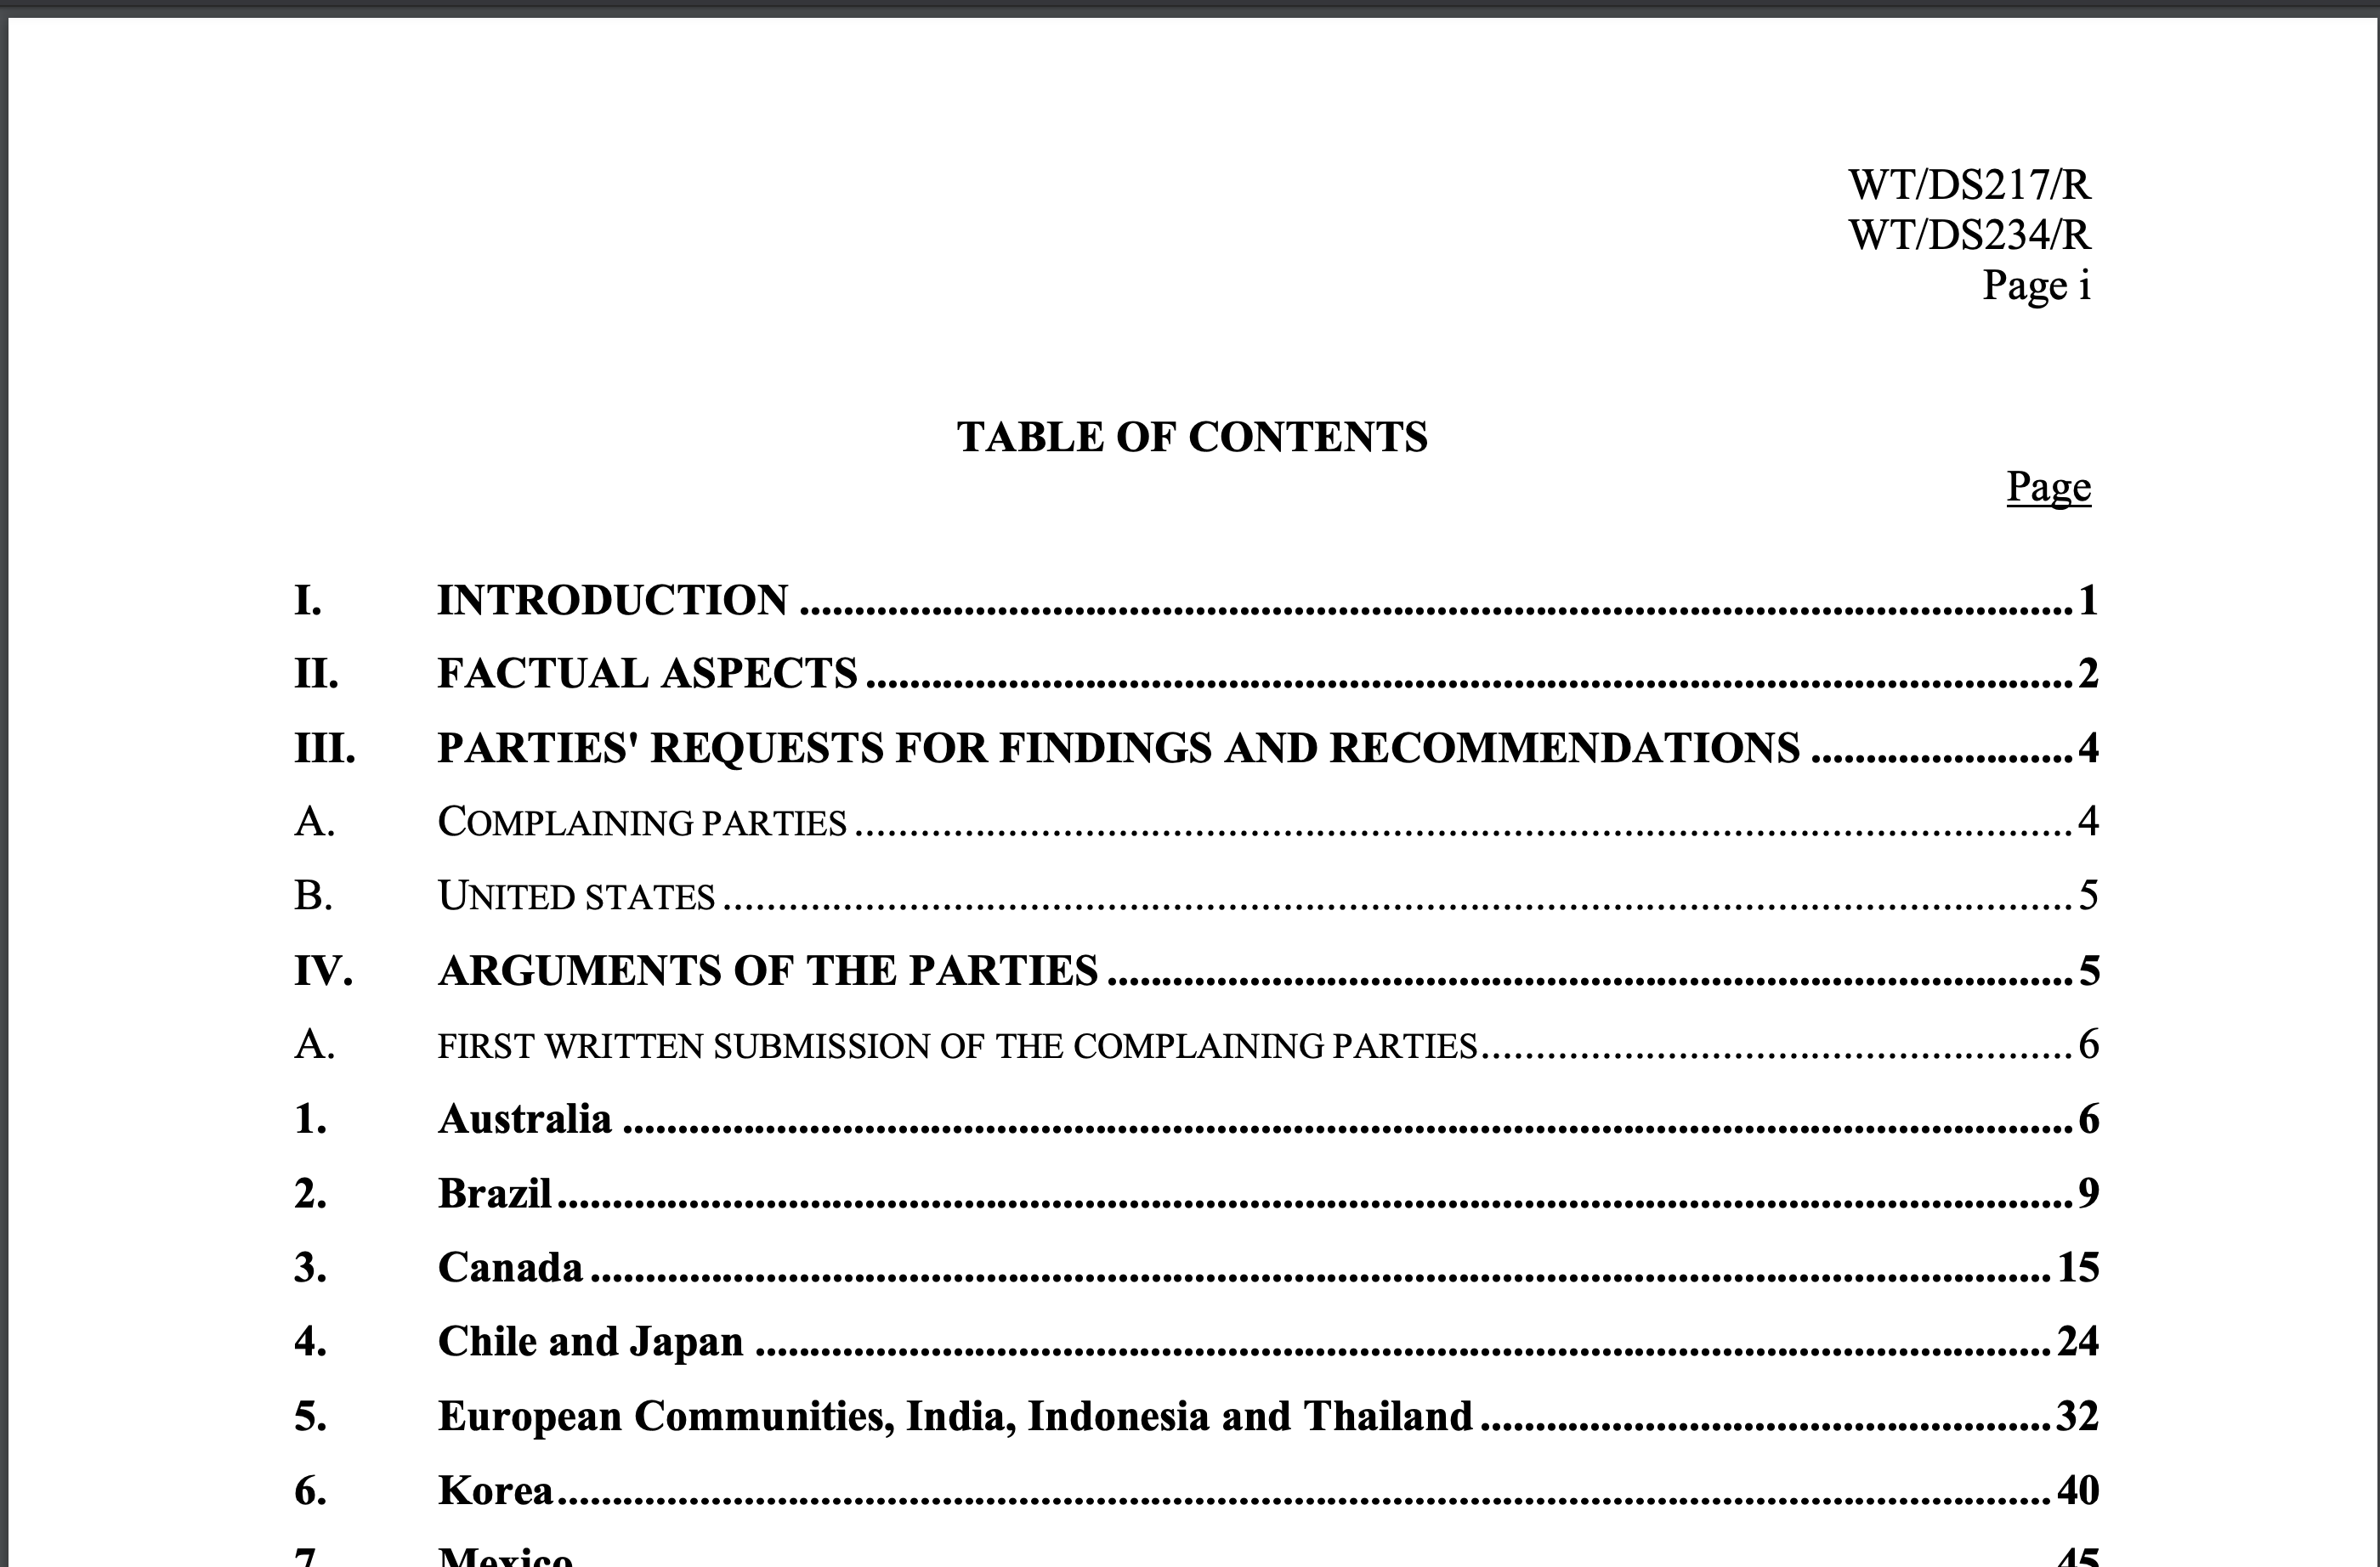
\includegraphics[scale=0.28]{Data/pngs/panel_report_toc.png}
    \caption{
        {\bf Table of Contents of Panel Report: }Panel provides 
        factual aspect in the panel report with its page location.
        }
    \label{fig:panel-report-toc}
\end{figure}
% \begin{center}
%     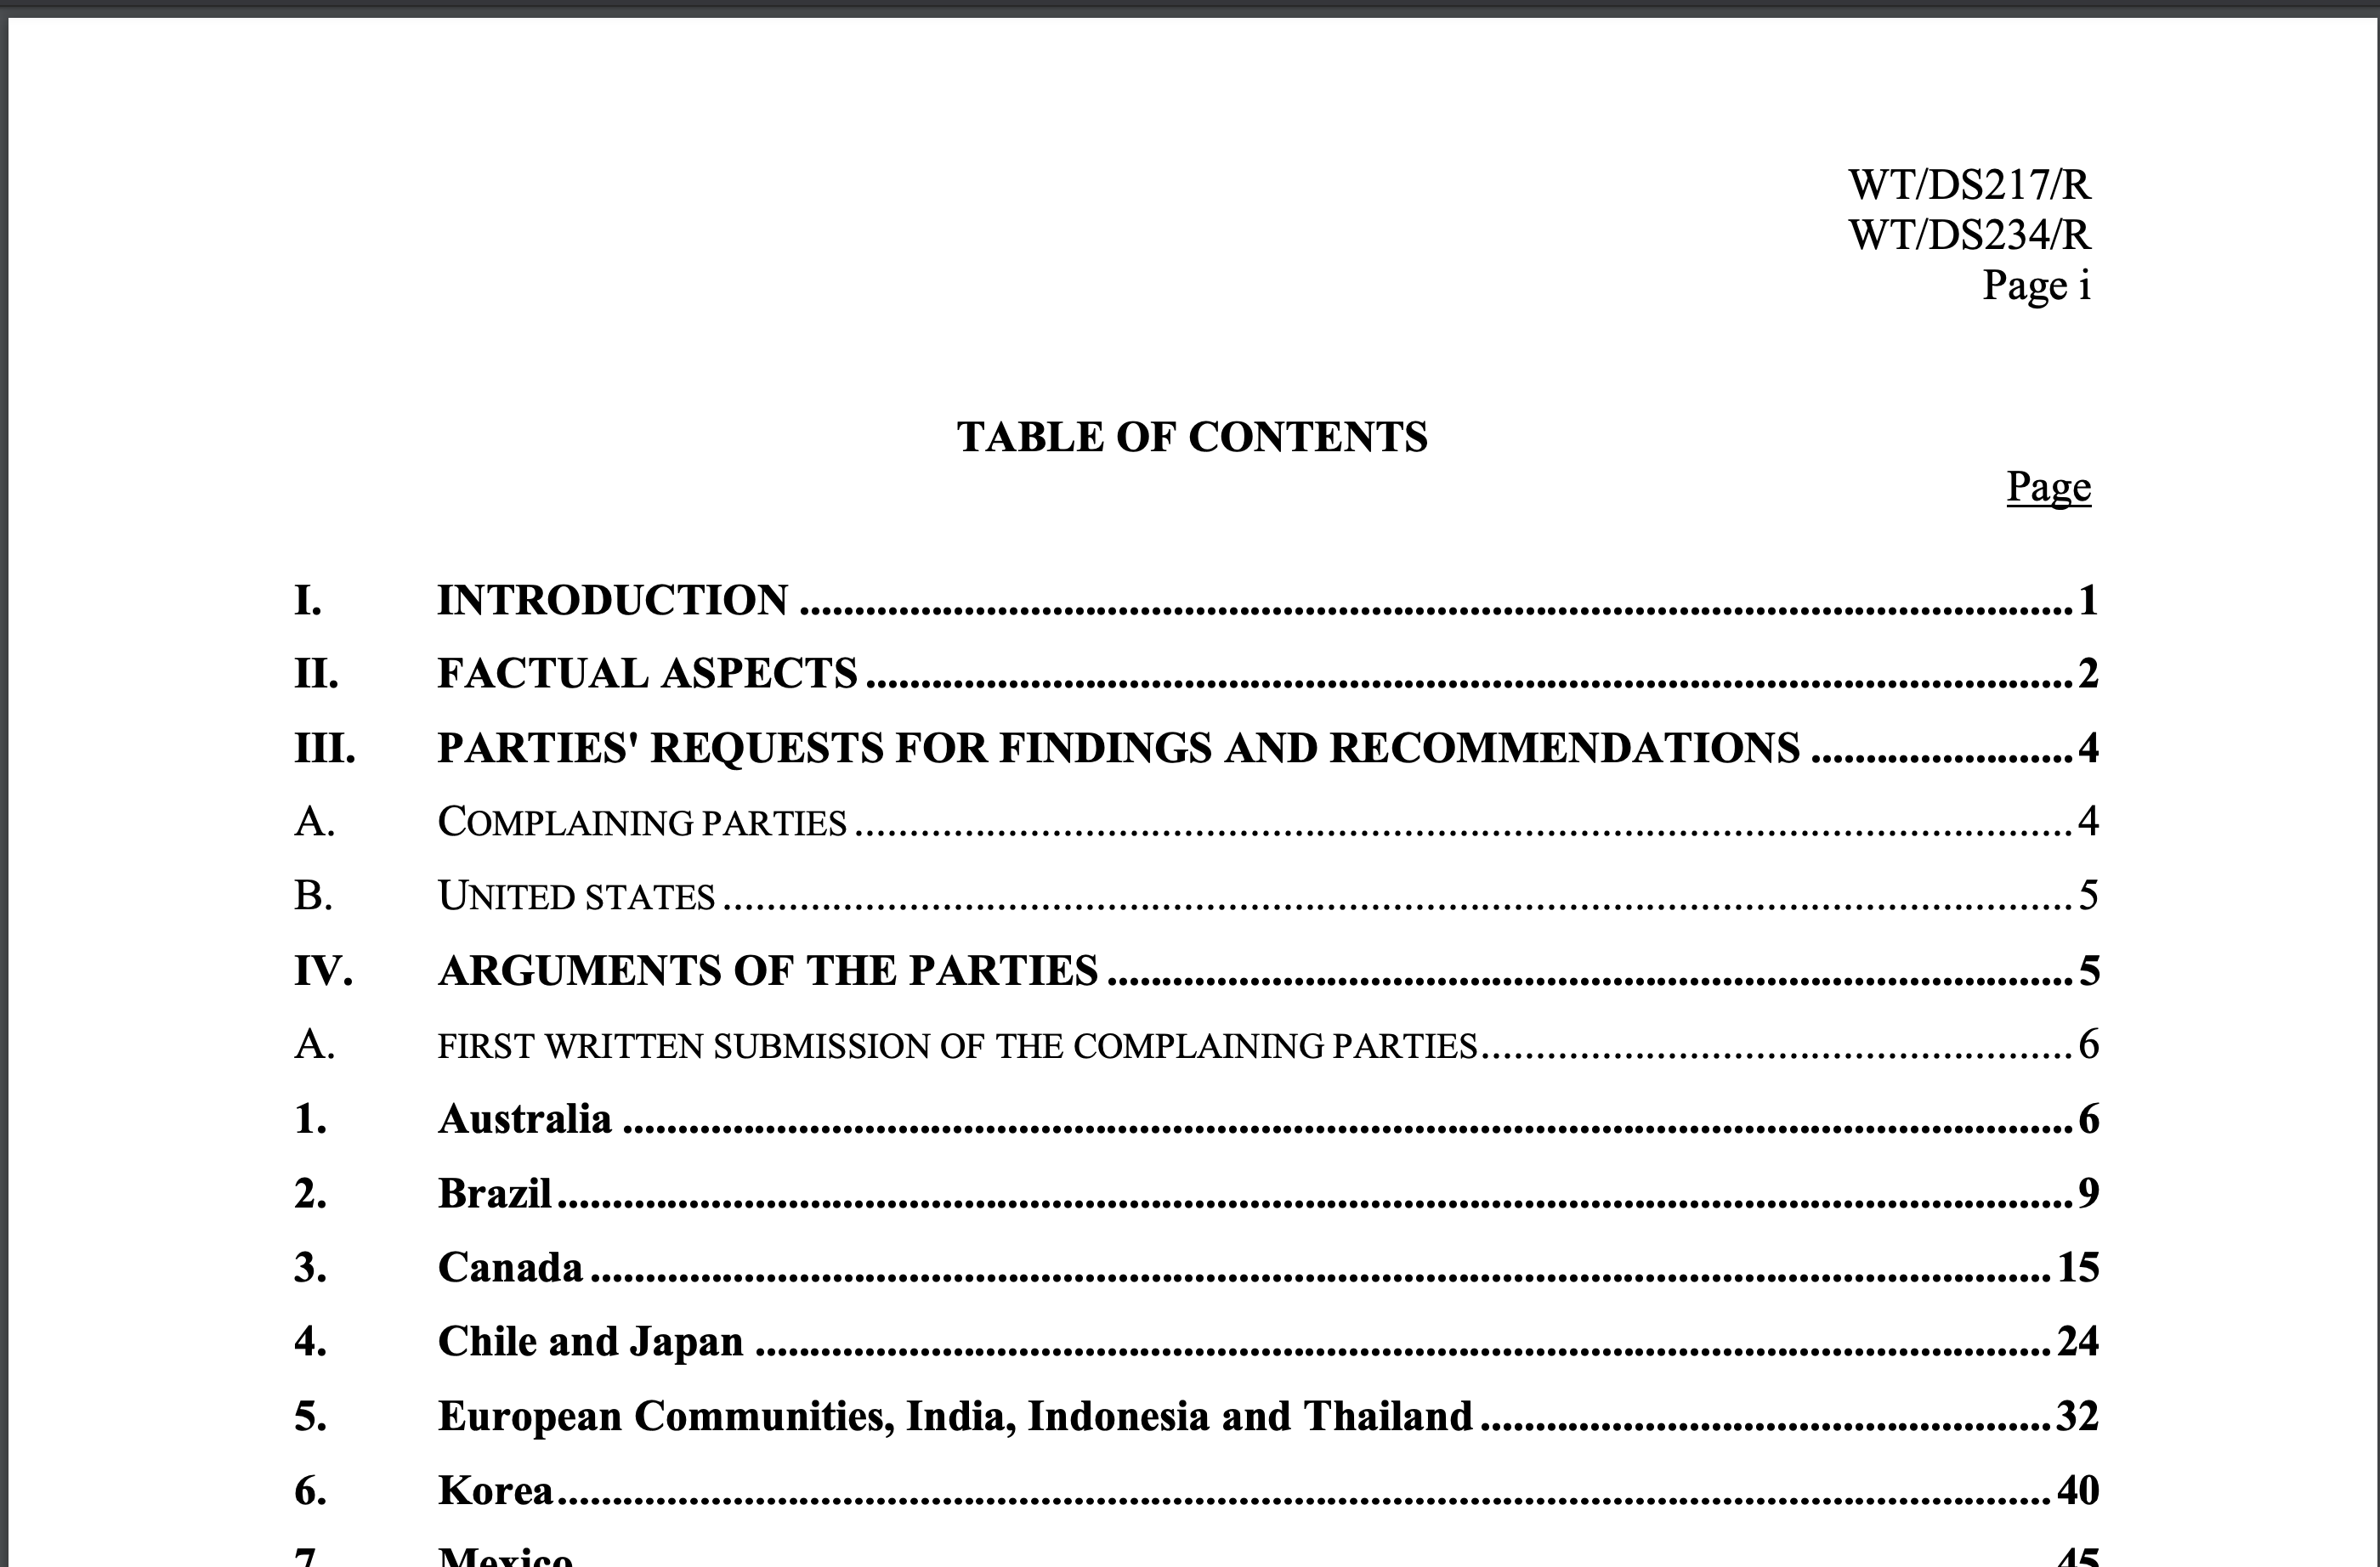
\includegraphics[scale=0.3]{Data/pngs/panel_report_toc.png}
% \end{center}

 
 



\subsection{Factual Aspect: Textual Description of the Dispute}
Textual description of trade policy that 
led to the dispute is formally called 
\textit{Factual Aspect} in WTO DSB. 
Since panels
always provide a factual aspect
that summarizes the content of the dispute
in the panel report (Figure \ref{fig:panel-report-toc}),
this paper wrote a program that can 
automatically search and collect 
the panel reports in the WTO official doucment website\footnote{
    \url{http://docs.wto.org}
}.
Then I wrote another program that locates the start 
and end page of the factual asepct using the information in the 
table of contents of the report (Figure \ref{fig:panel-report-toc}).
By using this location, I excerpted factual aspect 
from the panel reports. 
\hyperref[sub:factual-aspect-example]{Appendix A.1} shows an
example of excerpted factual aspect.



% way before they express their
% legal conclusion as to the inconsistency  to the rules of the WTO or not.

% where the panel expresses 
% its conclusion as to whether the challenged 
% trade policy is inconsistent to the rules of the WTO or not.

\subsection{Cited Articles: Set of Articles Cited for the Same Dispute}
Every lawsuit in WTO DSB 
has its own set of aritcles cited by complainant(s)
as shown in Table 
\ref{xltabular:cited-article-for-us-offset}. 
I wrote a program that collects a set of articles cited for 
each case from the WTO official webpage\footnote{\url{https://www.wto.org/english/tratop_e/dispu_e/dispu_status_e.htm}}. 
The webpage chronologically lists up all dispute cases
requested to WTO DSB and the prgoram visits each dispute page of 143 cases
and collects cited articles for each case. Among all the articles from different agreements
of the WTO agreements\footnote{
    WTO agreeemnts is comprised of mutiple agreements such as
    General Agreement on Tariffs and Trade 1994,
    Agreement on Agriculture,
    Agreement on the Application of Sanitary and Phytosanitary Measures,
    Agreement on Textiles and Clothing,
    Agreement on Technical Barriers to Trade,
    Agreement on Trade-Related Investment Measures,
    Agreement on Implementation of Article VI of the General Agreement on Tariffs and Trade 1994 (antidumping),
    Agreement on Subsidies and Countervailing Measures,
    Agreement on Rules of Origin,
    Agreement on Safeguards and so on.
    } ,
this paper collected articles from General Agreement on Tariffs and Trade 1994 (GATT 1994) only. 
This is because articles in GATT 1994 constitutes basic set of trade rules of WTO and other agreements 
elaborates the articles of GATT 1994 more in detail \citep{world1999wto}. For example, the official name of \textit{Agreement on Anti-dumping}
is \textit{Agreement on Implementation of Article VI of the General Agreement on Tariffs and Trade 1994}
where the name self-explains that it elaborates on the specific article of GATT 1994.
The collected result is listed in the \hyperref[sub:cited-articles-table]{Appendix A.2} and Figure \ref{fig:set-of-articles-used} 
lists up 80 different articles of GATT 1994 cited in 143 cases without duplication. 

\begin{figure}[h]
    \begin{quote}
    I, 
    I:1, 
    II, 
    II:1, 
    II:1(a), 
    II:1(b), 
    II:2, 
    II:3, 
    III, 
    III:1, 
    III:2, 
    III:4, 
    III:5, 
    III:7, 
    IV, 
    IX, 
    IX:2, 
    V, 
    V:1, 
    V:2, 
    V:3, 
    V:3(a), 
    V:4, 
    V:5, 
    V:6, 
    V:7, 
    VI, 
    VI:1, 
    VI:2, 
    VI:2(a), 
    VI:2(b), 
    VI:3, 
    VI:5(a), 
    VI:6, 
    VII, 
    VII:1, 
    VII:2, 
    VII:5, 
    VIII, 
    VIII:1, 
    VIII:3, 
    VIII:4, 
    X, 
    X:1, 
    X:2, 
    X:3, 
    X:3(a), 
    XI, 
    XI:1, 
    XIII, 
    XIII:1, 
    XIII:2, 
    XIII:3(b), 
    XIX, 
    XIX:1, 
    XIX:2, 
    XIX:3, 
    XV, 
    XVI, 
    XVI:1, 
    XVI:4, 
    XVII, 
    XVII:1, 
    XVII:1(c), 
    XVIII, 
    XVIII:10, 
    XVIII:11, 
    XX, 
    XXI, 
    XXII, 
    XXII:1, 
    XXIII, 
    XXIII:1, 
    XXIII:1(a), 
    XXIII:1(b), 
    XXIV, 
    XXIV:12, 
    XXIV:5(b), 
    XXIV:6, 
    XXVIII
    \end{quote}
    \caption{\textbf{Set of articles of GATT 1994 used in this paper: } The neural network is trained with textual content of each article.}
    \label{fig:set-of-articles-used}
\end{figure}

\subsubsection{Various Levels of Scope in Cited Articles}
As shown in Figure \ref{fig:set-of-articles-used}, 
members sometimes
cite articles in different levels of scope. For example, 
For the Article VI, member sometimes cites
Article VI as a whole but sometimes cites
Article VI:2 or Article VI:2(a).
This is because two main judicial bodies of WTO DSB, Panel and Appellate Body, 
both constitutes its jurisprudence using
various level of scope to interpret the legal texts of the WTO agreements,
such as in the level of \textit{Title, Article, Paragraph, Sentence or Term} as shown in Table {\ref{xltabular:level-of-scopes}}. 
Following this jurisprudence, members also cite articles in different levels of scope to 
make their legal claim fit and valid as much as possible.
\clearpage
\begin{xltabular}{\linewidth}{lXX}
    \hline
    \textbf{\normalsize Scope} 
    & \textbf{\normalsize Quote}
    & \textbf{\normalsize Source}
    \\
    \endfirsthead
    \hline \hline


    Title
    & ``As the \textbf{\textit{title}
    of Article 21 makes clear}, 
    the task of panels \ldots
    forms part of the process
    of the `Surveillance of 
    Implementation of the 
    Recommendations and Rulings' of the
    DSB. \ldots'' 
    & Appellate Body Report, \textit{US – Shrimp (Malaysia)}, paras. 86-87.
    \\
    \hline
    Article 
    &  ``The sequence of steps indicated above in the analysis of a claim of justification under \textbf{Article XX} reflects, not inadvertence or random choice, but rather the fundamental structure and logic of Article XX. \ldots''
    & Appellate Body Report, \textit{US – Shrimp (Malaysia)}, paras. 119-120.
    \\
    \hline
    Paragraph
    &  ``The verb 'may' in \textbf{Article VI:2} of the GATT 1994 is, in our opinion, properly
    understood as giving Members a choice between imposing an anti-dumping duty or
    not, as well as a choice between imposing an anti-dumping duty equal to the dumping
    margin or imposing a lower duty. \ldots''
    & Appellate Body Report, \textit{US – 1916 Act}, paras. 116.     
    \\
    \hline
    Sentence 
    & ``The customary rules of interpretation of public international law as
    required by \textbf{the first sentence of Article 17.6(ii) of the Anti-Dumping Agreement}, do
    not admit of another interpretation as far as the issue of zeroing raised in this appeal
    is concerned.''
    & Appellate Body Report, \textit{US – Zeroing (EC)}, paras. 132-133.
    % \hline
    % \textbf{\normalsize Scope} 
    % & \textbf{\normalsize Quote}
    % & \textbf{\normalsize Source}
    \\
    \hline
    Term
    & ``Article II:1(a) provides that a
    Member shall accord to the `commerce' of other Members treatment no less
    favourable than that provided for in its Schedule. \textbf{The term `commerce'} is defined as
    referring broadly to the exchange of goods such that, in this provision, the 'commerce'
    of a Member should be understood to refer to all such exchanges of that Member''
    & Appellate Body Report, \textit{Colombia – Textiles}, para. 5.34.
    \\
    \hline
    \caption{Various levels of scope appearing in the jurisprudence of WTO DSB}
    \label{xltabular:level-of-scopes}

\end{xltabular}


% \begin{figure}[h]
% \begin{quote}
%     \ldots As the \textit{title} of Article 21 makes clear, the task of panels \ldots
%      forms part of the process
%     of the 'Surveillance of Implementation of the Recommendations and Rulings' of the
%     DSB. - \textit{Appellate Body Report, US – Shrimp (Malaysia), paras. 86-87. }
% \end{quote}
% \caption{Various Interpretative Scopes of Panel and Appellate Body}
% \end{figure}

% paragraph is also important in terms of scope.



% == METHOD ==
\section{Methodology: Considerations and Development}
This section introduces two main considerations to design the method used in this paper.
Then it explains the method that is used to fit the network of articles of WTO agreement under those considerations.


\subsection{Two Main Considerations For Design of Method} \label{justification-nn}
This paper considered two main points to
determine its method to qualitatively fit a set of edge weight $W$ for the \textit{directed weighted graph} $G$ defined in Figure \ref{fig:def}. One is importance of using the information represented in a form of textual description inside the content of dispute and legal article as exemplified in \hyperref[sub:factual-aspect-example]{Appendix A.1} and Figure {\ref{fig:gatt_art1}} respectively. The other one is about the way to generalize each member's startegic citation pattern. Since members of the WTO strategically cite
the articles of WTO agreement expecting different outcomes thats serves member-specific national interest \citep{who_gets, pelc, latent}, this paper
selected a method that can generalize this member speicific citation pattern. These two considerations and the solution will be explained in the following subsections.
% == HEATMAP MATRIX == 
\begin{figure}[ht]
    \begin{subfigure}[b]{0.49\textwidth}
        \centering{
            \resizebox{\textwidth*\real{\heatmap}}{\textwidth*\real{\heatmap} * \real{1}}{% This file was created by tikzplotlib v0.9.4.
\begin{tikzpicture}

\begin{axis}[
tick align=outside,
tick pos=left,
title={coo},
x grid style={white!69.0196078431373!black},
xmin=0, xmax=58,
xtick style={color=black},
y grid style={white!69.0196078431373!black},
ymin=0, ymax=58,
ytick style={color=black}
]
\addplot graphics [includegraphics cmd=\pgfimage,xmin=0, xmax=58, ymin=0, ymax=58] {coo-001.png};
\end{axis}

\end{tikzpicture}
}
            \caption{$W_{\text{co-cites}}$}
            \label{subfig:adj_sparse}
        }
    \end{subfigure}
    % \hfill
    % \pgfdeclareverticalshading{colormap}{0.2cm}{rgb(0.0pt)=(0,1,1); rgb(6cm)=(0.8784,0.6902,0.99998)}
    % \pgfuseshading{colormap}
    \hfill
    \begin{subfigure}[b]{0.49\textwidth}
        \centering{
            \resizebox{\textwidth*\real{\heatmap}}{\textwidth*\real{\heatmap} * \real{1}}{% This file was created by tikzplotlib v0.9.4.
\begin{tikzpicture}

\begin{axis}[
hide x axis,
hide y axis,
tick align=outside,
tick pos=left,
x grid style={white!69.0196078431373!black},
xmin=0, xmax=80,
xtick style={color=black},
y grid style={white!69.0196078431373!black},
ymin=0, ymax=80,
ytick style={color=black}
]
\addplot graphics [includegraphics cmd=\pgfimage,xmin=0, xmax=80, ymin=0, ymax=80] {coo_dense-002.png};
\end{axis}

\end{tikzpicture}
}
            \caption{$W_{\text{text}}$}
            \label{subfig:adj_dense}
        }
    \end{subfigure}
    \label{fig:sparse_dense}
    \vfill
    \centering{
        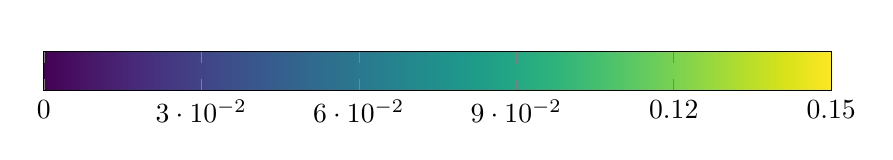
\begin{tikzpicture}
    \begin{axis}[
            hide axis,
            scale only axis,
            height=0pt,
            width=0pt,
            colormap/viridis,
            colorbar horizontal,
            point meta min=0,
            point meta max=0.15,
            colorbar style={
                    width=10cm,
                    height=0.5cm,
                    xtick={0,0.03,0.06,0.09,0.12,0.15}
                }]
        \addplot [draw=none] coordinates {(0,0)};
    \end{axis}
\end{tikzpicture}
    }
    \caption{\textbf{Heatmap of Two Different Edge Weight Matrices: }Above two subfigures visualizes two different \textit{edge weight matrices} $W_{\text{co-cites}}$ and $W_{\text{text}}$. One can check that $W_{\text{co-cites}}$ is sparser than $W_{\text{text}}$.}
    \label{fig:heatmap:edgeweights:compare}
\end{figure}



\subsubsection{Importance of Using Textual Information}
I emphasizes the necessity of using textual information
to qualitatively fit the edge weight matrix $W^*$ as defined in Section \ref{subsec:def}. 
Rather than using the textual data, one can simply model the co-citation matrix as $W^*$, which counts the co-occurrences of each article with other articles.
% pattern between the articles of WTO agreements that counts the co-occurrences of each article with other articles, however,
However, it simply allocates a large edge weight for frequently cited articles and fails to explain how articles systematically interact with other articles.
This failure is mainly due to the insufficient information in the co-citation matrix. Members cite the articles of
the WTO agreements based on the complex characteristics of
the trade policy that led to the dispute. 
However, the co-citation pattern omits this contextual information . To emphasize the necessity of using the textual information, I prepared two different matrices $W_{\text{co-cites}}$ and $W_{\text{text}}$ that are both following the definition of \textit{edge weight matrix} $W$ in Section \ref{subsec:def}.
$W_{\text{co-cites}}$ is calculated using the co-citation pattern between the articles of the WTO agreements as formally defined
%  \textit{Normalized Co-citation Matrix} 
in Figure %\ref{fig:def-illus-co-cites} and 
\ref{fig:def-illus-normal-co-cites}.
$W_{\text{text}}$ is the one fitted using the textual information and the way how it's fitted will be explained at the following bodies of this section, in particular in Section \ref{subsec:rf}.
Two heatmaps visualized in Figure \ref{fig:heatmap:edgeweights:compare} shows how sparse the $W_{\text{co-cites}}$ is compared to the $W_{\text{text}}$. This sparsity indirectly refers to the insufficient information
to qualitatively map the jurisprudence of WTO DSB.
% and I will introduce the failure of the weight fitting algorithm using \textit{Random Forest} in case of using this sparse matrix $W_{\text{co_cites}}$.
In contrast with it, if we fit the \textit{edge weight matrix} $W$ using the textual information, we get a more dense and informative matrix as visualized in Figure \ref{subfig:adj_dense}.
% and visualized them as a heatmap in Figure \ref{fig:heatmap:edgeweights:compare}.
% $W_{\text{co-cites}}$ is an edge weight matrix that is calculated only using the co-citation pattern between articles without textual information.
% We can compare two weight matrices of each network that maps the regulatory system of WTO DSB as a network of articles of WTO agreements in Figure \ref{fig:sparse_dense}.
% % == DEF EXAMPLE == 
\begin{figure}[h]
    \begin{subfigure}[b]{1\textwidth}
        \[\text{Let } \delta^d_{ij} \text{ is defined to be } 1 \text{ if } \{(v_i, v_j) \mid v_i, v_j \in V \text{ and } i \neq j \} \subset c_{d \in D} \ \text{ else } 0\]
        \[\text{ where } V, D \text{ and } c_d \text{ is defined as in Figure \ref{fig:def:set-of-cited-articles}}. \]
        \[\text{Then let \textit{co-citation matrix} } M = (m_{ij}) \in \Bbb{N}^{|V| \times |V|} \text{ s.t. } m_{ij} = \sum_{d \in D}\sum_{i,j \in V}\delta^d_{ij}\]
        \caption{\textbf{Formal Definition of Co-citation Matrix}}
        \label{subfig:co-cites:def}
    \end{subfigure}
    \vfill
    \begin{subfigure}[b]{1\textwidth}
        \centering{
            % \begin{figure}[h]
%     \centering
    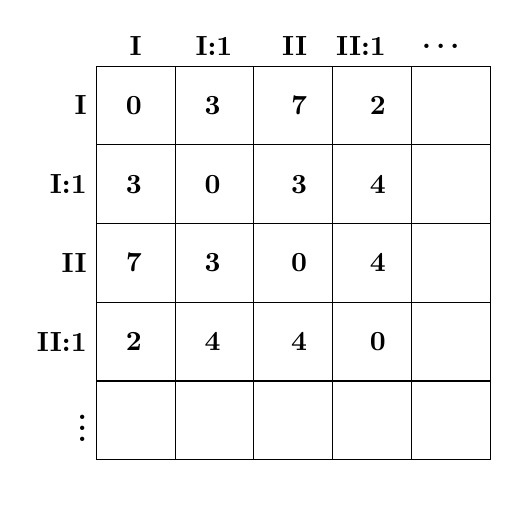
\begin{tikzpicture}
        \foreach \i in {\xMin,...,5} {
            \draw [black] (\i,4) -- (\i,9) node [below] at (\i,4) {};
        }
        \foreach \i in {4,...,9} {
            \draw [black] (\xMin,\i) -- (5,\i) node [left] at (\xMin,\i) {};
        }

        % \node [left] at (0,0.5) {\textbf{XXVIII}};
        % \node [left] at (0,1.5) {\textbf{XXVI:6}};
        % \node [left] at (0,2.5) {\textbf{XXIV:5(b)}};
        % \node [left] at (0,3.5) {\textbf{XXIV:12}};
        \node [left] at (0,4.5) {\textbf{\vdots}};
        \node [left] at (0,5.5) {\textbf{II:1}};
        \node [left] at (0,6.5) {\textbf{II}};
        \node [left] at (0,7.5) {\textbf{I:1}};
        \node [left] at (0,8.5) {\textbf{I}};

        % \node [left] at (8.8, 9.25) {\textbf{XXVIII}};
        % \node [left] at (7.8, 9.25) {\textbf{XXVI:6}};
        % \node [left] at (6.8, 9.25) {\textbf{XXIV:5(b)}};
        % \node [left] at (5.8, 9.25) {\textbf{XXIV:12}};
        \node [left] at (4.8, 9.25) {\textbf{\ldots}};
        \node [left] at (3.8, 9.25) {\textbf{II:1}};
        \node [left] at (2.8, 9.25) {\textbf{II}};
        \node [left] at (1.85, 9.25) {\textbf{I:1}};
        \node [left] at (0.7,9.25) {\textbf{I}};

        \node [left] at (0.7,8.5) {\textbf{0}};
        \node [left] at (1.7,8.5) {\textbf{3}};
        \node [left] at (2.8,8.5) {\textbf{7}};
        \node [left] at (3.8,8.5) {\textbf{2}};
        
        \node [left] at (0.7,7.5) {\textbf{3}};
        \node [left] at (1.7,7.5) {\textbf{0}};
        \node [left] at (2.8,7.5) {\textbf{3}};
        \node [left] at (3.8,7.5) {\textbf{4}};

        \node [left] at (0.7,6.5) {\textbf{7}};
        \node [left] at (1.7,6.5) {\textbf{3}};
        \node [left] at (2.8,6.5) {\textbf{0}};
        \node [left] at (3.8,6.5) {\textbf{4}};

        \node [left] at (0.7,5.5) {\textbf{2}};
        \node [left] at (1.7,5.5) {\textbf{4}};
        \node [left] at (2.8,5.5) {\textbf{4}};
        \node [left] at (3.8,5.5) {\textbf{0}};



        % \node [left] at (5.5,9.5) {\textbf{Embedding Dimension = $k$}};
        % \node [right, rotate=-90, font=\small] at (6.5,7) {\textbf{Max Sequence Length = $n$}};


    % \draw [step=1.0,blue, very thick] (0.5,0.5) grid (5.5,4.5);
    % \draw [very thick, brown, step=1.0cm,xshift=-0.5cm, yshift=-0.5cm] (0.5,0.5) grid +(5.5,4.5);
    \end{tikzpicture} 
%     \label{fig:visualize-co-cites}      
%     \caption{\textbf{Definition of Co-citation Matrix:} This paper defines co-citation matrix $C$ as a $\mid V \mid \times \mid V \mid$ matrix where each element $c_{ij}:= \text{Counts of } $ is count of all co-occurrence $  \text{ } s.t. \text{ } \forall i,j \in \mid V \mid$ } 
% \end{figure}

% This  dispute  concerns  the  Continued  Dumping 
            \caption{\textbf{Illustration of Co-citation Matrix}}
            \label{subfig:co-cites:illus}
        }
    \end{subfigure}
    \label{fig:def-illus-co-cites}      
    \caption{\textbf{Formal Definition and Illustration of Co-citation Matrix:} This paper defines co-citation matrix $M$ as subfigure $(a)$ and it is illustrated as subfigure $(b)$.} 
\end{figure}
\begin{figure}[t!]
    \begin{subfigure}[b]{1\textwidth}
        \[\text{For given $M$ defined in Figure \ref{subfig:co-cites:def},} \]
        \[\text{let \textit{normalized co-citation matrix} } N = (n_{ij}) \in \Bbb{R}^{|V| \times |V|} \text{ s.t. } n_{ij} = \frac{m_{ij}}{\sum_{j \in V}m_{ij}} \]
        \caption{\textbf{Formal Definition of Normalized Co-citation Matrix}}
        \label{subfig:co-cites:def:normal}
    \end{subfigure}
    \vfill
    \begin{subfigure}[b]{1\textwidth}
        \centering{
            % \begin{figure}[h]
%     \centering
    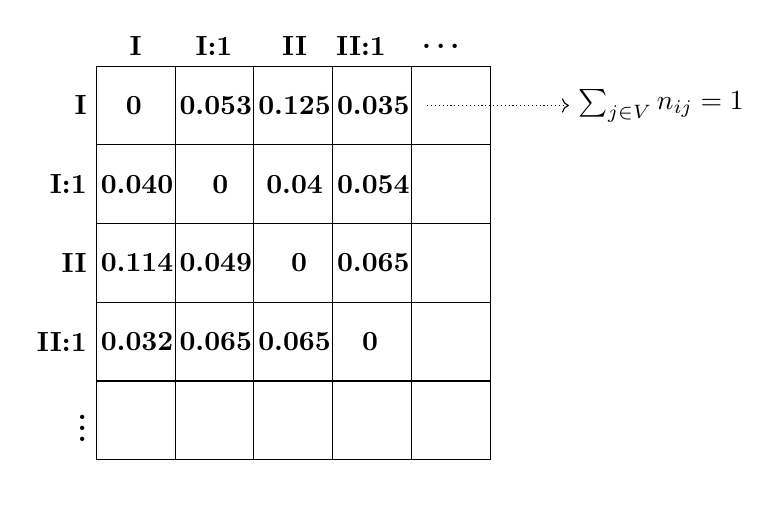
\begin{tikzpicture}
        \foreach \i in {\xMin,...,5} {
            \draw [black] (\i,4) -- (\i,9) node [below] at (\i,4) {};
        }
        \foreach \i in {4,...,9} {
            \draw [black] (\xMin,\i) -- (5,\i) node [left] at (\xMin,\i) {};
        }

        % \node [left] at (0,0.5) {\textbf{XXVIII}};
        % \node [left] at (0,1.5) {\textbf{XXVI:6}};
        % \node [left] at (0,2.5) {\textbf{XXIV:5(b)}};
        % \node [left] at (0,3.5) {\textbf{XXIV:12}};
        \node [left] at (0,4.5) {\textbf{\vdots}};
        \node [left] at (0,5.5) {\textbf{II:1}};
        \node [left] at (0,6.5) {\textbf{II}};
        \node [left] at (0,7.5) {\textbf{I:1}};
        \node [left] at (0,8.5) {\textbf{I}};

        % \node [left] at (8.8, 9.25) {\textbf{XXVIII}};
        % \node [left] at (7.8, 9.25) {\textbf{XXVI:6}};
        % \node [left] at (6.8, 9.25) {\textbf{XXIV:5(b)}};
        % \node [left] at (5.8, 9.25) {\textbf{XXIV:12}};
        \node [left] at (4.8, 9.25) {\textbf{\ldots}};
        \node [left] at (3.8, 9.25) {\textbf{II:1}};
        \node [left] at (2.8, 9.25) {\textbf{II}};
        \node [left] at (1.85, 9.25) {\textbf{I:1}};
        \node [left] at (0.7,9.25) {\textbf{I}};

        \node [left] at (0.7,8.5) {\textbf{0}};
        \node [left] at (2.1,8.5) {\textbf{0.053}};
        \node [left] at (3.1,8.5) {\textbf{0.125}};
        \node [left] at (4.1,8.5) {\textbf{0.035}};
        
        \node [left] at (1.1,7.5) {\textbf{0.040}};
        \node [left] at (1.8,7.5) {\textbf{0}};
        \node [left] at (3,7.5) {\textbf{0.04}};
        \node [left] at (4.1,7.5) {\textbf{0.054}};

        \node [left] at (1.1,6.5) {\textbf{0.114}};
        \node [left] at (2.1,6.5) {\textbf{0.049}};
        \node [left] at (2.8,6.5) {\textbf{0}};
        \node [left] at (4.1,6.5) {\textbf{0.065}};

        \node [left] at (1.1,5.5) {\textbf{0.032}};
        \node [left] at (2.1,5.5) {\textbf{0.065}};
        \node [left] at (3.1,5.5) {\textbf{0.065}};
        \node [left] at (3.7,5.5) {\textbf{0}};

        \draw[->, densely dotted, thin] (4.2,8.5) -- (6,8.5) node[right] {$\sum_{j \in V} n_{ij} = 1$};

        % \node [left] at (10,8.5) {-> \textbf{Embedding Dimension = $k$}};
        % \node [right, rotate=-90, font=\small] at (6.5,7) {\textbf{Max Sequence Length = $n$}};


    % \draw [step=1.0,blue, very thick] (0.5,0.5) grid (5.5,4.5);
    % \draw [very thick, brown, step=1.0cm,xshift=-0.5cm, yshift=-0.5cm] (0.5,0.5) grid +(5.5,4.5);
    \end{tikzpicture} 
%     \label{fig:visualize-co-cites}      
%     \caption{\textbf{Definition of Co-citation Matrix:} This paper defines co-citation matrix $C$ as a $\mid V \mid \times \mid V \mid$ matrix where each element $c_{ij}:= \text{Counts of } $ is count of all co-occurrence $  \text{ } s.t. \text{ } \forall i,j \in \mid V \mid$ } 
% \end{figure}

% This  dispute  concerns  the  Continued  Dumping 
            \caption{\textbf{Illustration of Noramlized Co-citation Matrix}}
            \label{subfig:co-cites:illus:normal}
        }
    \end{subfigure}
    \caption{\textbf{Formal Definition and Illustration of Normalized Co-citation Matrix:} This paper defines normalized co-citation matrix $N$ of $M$ as subfigure $(a)$ and it's illustrated as subfigure $(b)$ using the paper's dataset. Note that normalized co-citation matrix is no more \textit{symmetric}, $n_{ij} \neq n_{ji} \text{ } \forall i,j \in V$. This definition is prepared to fit the definition of co-citation matrix to that of $W$ as defined in Section \ref{subsec:def}.} 
    \label{fig:def-illus-normal-co-cites}
\end{figure}
Upon this observation, this paper justifies the use of a deep neural network to process information embedded in the text description of the dispute and regulatory content of the articles. 
This is because the deep neural network is known to effectively
extract information from the textual data to perform various tasks such as text classification \citep{minaee2020deep}, text summarization \citep{textsum} and text generation \citep{guo2017long}.
% This paper will compare two different results that one uses textual information using deep learning and the other one
% uses the frequency of co-citation only after explaining how deep learning works to encompass the textual information.
% if a method
% do not consider a way to encompass the information
% about the identiy of the trade policy at issue with
% each article's regulatory content written in its own article text,
% it can only reflect how articles of WTO agreements are co-cited
% together rather than reflecting how articles of WTO agreements
% cooperates to regulate each charactersitic of complex trade policy that led to the dispute.
 
 
 



\subsubsection{Generalization of Each Member's Strategic Citation}

This paper aims to map the regulatory system of WTO DSB in a form of \textit{directed weighted graph} $G$ as defined in Figure \ref{fig:def}.
To achieve this purpose, we need to fit $W$ to generalize member specific strategic citation behavior.
In terms of generalization, deep neural network is known to generalize well despite
its large capacity \citep{neyshabur2017exploring}, possible instability of training algorithm \citep{charles2017stability}, nonrobustness \citep{zahavy2017ensemble}, and sharp minima \citep{dinh2017sharp}.
Therefore this paper trains a deep neural network without any member specific information such as geolocation, GDP or specialized industry and so on. By training a deep neural network only using a description of the possible inconsistent trade policy and the legal text of the cited articles,
this paper expects a fitted $G^{*} = (V, E, W^*)$ can show interactions between articles of the WTO agreements
without being biased to member specific strategic citation.

\subsection{Design of Deep Neural Network}
Upon the justification of using deep neural network with two main reasons explained in Section \ref{justification-nn}, %one is to effectively process the text information and the other one is to generalize member specific strategic citation,
I introduce a design of deep neural network that is expected to efficiently encode members' legal citation pattern.

\subsubsection{Design Input/Output of Deep Neural Network: by Analogy with How Member Cites in WTO DSB}
A rule of thumb to design input and output of deep neural network is to mimic 
how humans do for a given task. 
Therefore I present a visualization of how legal expert of rules of WTO determines whether to cite a legal article of WTO agreements with an example of \textit{Korea - Beef} case (Figure \ref{fig:viz:how-member-cites-citable} and Figure \ref{fig:viz:how-member-cites-non-citable}).
In this case, the United States raised a claim relating to the \textit{Dual-retail system} maintained by South Korea. In \textit{Dual-retail system}, South Korea maintained two distinct retail systems
for imported and domestic beef, i.e., there exist stores specialized for imported beef and they can sell only imported beef and cannot sell domestic beef. U.S. claimed that the \textit{Dual-retail system} is inconsistent to the Article III:4 (National Treatment) of GATT 1994 
because \textit{Dual-retail system} has a chance to discriminate domestic and imported beef. A measure that discriminates domestic and imported products falls under the scope of the Article III:4 of the GATT 1994, which states the principle of \textit{National Treatment} that prohibits the discrimination between imported and domestic \textit{like product}. However, U.S. didn't 
cite the Article I:1 of GATT 1994 that prohibits the discrimination between members of WTO agreements
because \textit{Dual-retail system} didn't discriminate the United States with other countries that exports beef to South Korea, such as Argentina, Austrailia, etc.

We can understand that there exists a shared understanding over regulatory system of WTO DSB among legal experts of the rules of WTO. They follow up new cases and study jurisprudence stated in the \textit{Panel} or  \textit{Appellate Body} reports.
Then they organize a legal argument by citing certain article(s) upon this shared understanding for given possible inconsistent measure held by a member of WTO.

To mimic this reasoning process, I designed the input and output of the deep neural network as illustrated in Figure \ref{fig:design-of-nn}.
The neural network is designed to estimate the citable probability for given pair of a factual aspect and text of a legal article. 
By iteratively trains the neural network with data explained in Section \ref{sec:data}, I expect the neural network can learn a shared understanding over reglatory system of WTO DSB as closely as to that of legal experts.
The detailed structure of neural network and training technique will be explained in the later subsections.
% For total $11,440$ pairs of factual aspect and legal articles (143 different cases (Figure \ref{fig:ds-cases-used}) and 80 different legal articles (Figure \ref{fig:def:set-of-cited-articles})

\begin{figure}[ht]
    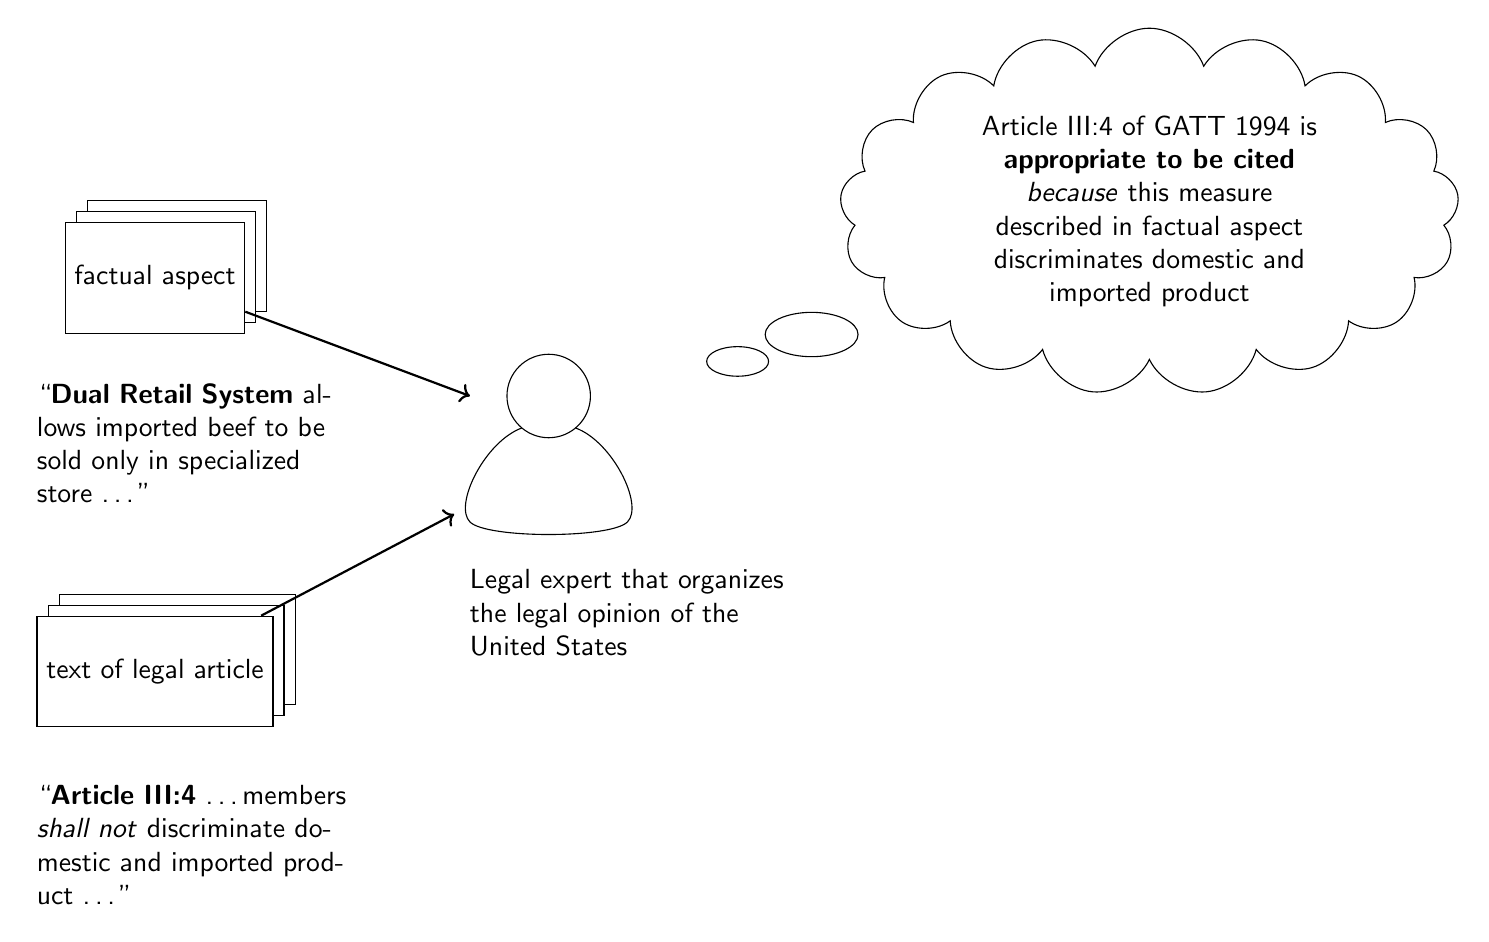
\begin{tikzpicture}[font=\sffamily,
      doc/.style={draw, minimum height=4em, minimum width=3em,
          fill=white,
          double copy shadow={shadow xshift=4pt,
              shadow yshift=4pt, fill=white, draw}},
    ]
    \begin{scope}[xshift=-8cm, yshift=2cm]
      \node[doc] at (0, 0) (factual) {factual aspect};
      \node[text width=4cm] at (0.5,-2.1) 
    {``\textbf{Dual Retail System} allows imported beef to be sold only in specialized store \ldots ''};
      
      \node[doc] at (0, -5)(legal-article) {text of legal article};
      \node[text width=4cm] at (0.5,-7.2)
      {``\textbf{Article III:4} \ldots members \textit{shall not} discriminate domestic and imported product \ldots''};
  
  
      % human torso with head
      \begin{scope}[xshift=5cm, yshift=-1.5cm]
        \draw (0,0) circle (.53);
        \draw (-130:.53) .. controls +(200:.5) and
        +(-45:-.3) .. (-1,-1.6) .. controls +(-45:.3) and
        +(45:-.3) .. (1,-1.6) .. controls +(45:.3) and
        +(-20:.5) .. (-50:.53);
      \end{scope}
      \node[text width=4cm] at (6,-4.25)
      {Legal expert that organizes the legal opinion of the United States};
  
  
      % arrows to feed factual and article content
      \begin{scope}[every edge/.append style={->}] % for directed edge, change "style={->, double=black, draw=white}]"
        \path[->] (factual) edge[thick,->] node[above, xshift=5pt] {} +(4,-1.5);
        \path[->] (legal-article) edge[thick,->] node[above, xshift=10pt] {} +(3.8,2);
      \end{scope}
  
      \begin{scope}[xshift=16cm, yshift=-1.5cm]
        \node [draw, align=center,
          cloud callout, 
          cloud puffs = 17, 
          cloud puff arc=140,
          callout pointer segments = 2, 
          anchor = pointer,
          callout relative pointer = {(200:2cm)},
          aspect = 2, 
          above left = 1.2 ]
        {Article III:4 of GATT 1994 is \\ \textbf{appropriate to be cited} \\ \textit{because} this measure \\ described in factual aspect \\ discriminates domestic and \\ imported product};
      \end{scope}      
    \end{scope}
  \end{tikzpicture}
  \caption{\textbf{Visualization of How Member Cites in WTO DSB (Citable Case): }With two different contexts, factual aspect and text of legal articles, member judges whether the given legal article is appropriate to be cited or not.}
  \label{fig:viz:how-member-cites-citable}   
  \end{figure}
    

\begin{figure}[ht]
  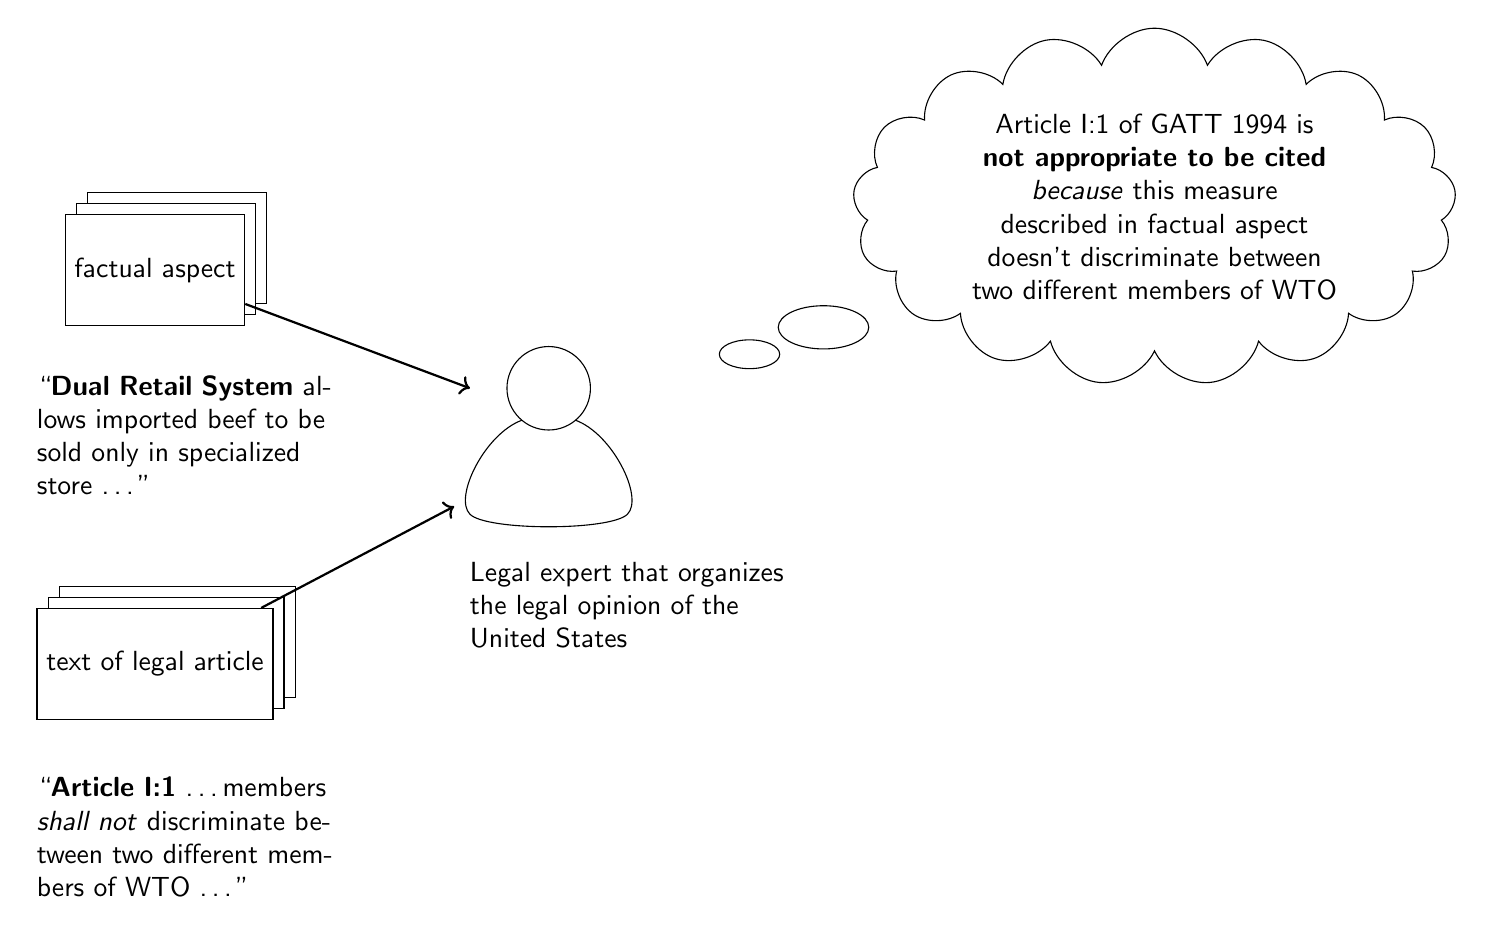
\begin{tikzpicture}[font=\sffamily,
    doc/.style={draw, minimum height=4em, minimum width=3em,
        fill=white,
        double copy shadow={shadow xshift=4pt,
            shadow yshift=4pt, fill=white, draw}},
  ]
  \begin{scope}[xshift=-8cm, yshift=2cm]
    \node[doc] at (0, 0) (factual) {factual aspect};
    \node[text width=4cm] at (0.5,-2.1) 
  {``\textbf{Dual Retail System} allows imported beef to be sold only in specialized store \ldots ''};
    
    \node[doc] at (0, -5)(legal-article) {text of legal article};
    \node[text width=4cm] at (0.5,-7.2)
    {``\textbf{Article I:1} \ldots members \textit{shall not} discriminate between two different members of WTO \ldots''};


    % human torso with head
    \begin{scope}[xshift=5cm, yshift=-1.5cm]
      \draw (0,0) circle (.53);
      \draw (-130:.53) .. controls +(200:.5) and
      +(-45:-.3) .. (-1,-1.6) .. controls +(-45:.3) and
      +(45:-.3) .. (1,-1.6) .. controls +(45:.3) and
      +(-20:.5) .. (-50:.53);
    \end{scope}
    \node[text width=4cm] at (6,-4.25)
    {Legal expert that organizes the legal opinion of the United States};


    % arrows to feed factual and article content
    \begin{scope}[every edge/.append style={->}] % for directed edge, change "style={->, double=black, draw=white}]"
      \path[->] (factual) edge[thick,->] node[above, xshift=5pt] {} +(4,-1.5);
      \path[->] (legal-article) edge[thick,->] node[above, xshift=10pt] {} +(3.8,2);
    \end{scope}

    \begin{scope}[xshift=16cm, yshift=-1.5cm]
      \node [draw, align=center,
        cloud callout, 
        cloud puffs = 17, 
        cloud puff arc=140,
        callout pointer segments = 2, 
        anchor = pointer,
        callout relative pointer = {(200:2cm)},
        aspect = 2, 
        above left = 1.2 ]
      {Article I:1 of GATT 1994 is\\ \textbf{not appropriate to be cited} \\ \textit{because} this measure \\ described in factual aspect \\ doesn't discriminate between \\ two different members of WTO };
    \end{scope}      
  \end{scope}
\end{tikzpicture}
\caption{\textbf{Visualization of How Member Cites in WTO DSB (Non-Citable Case): }With two different contexts, factual aspect and text of legal articles, member judges whether the given legal article is appropriate to be cited or not.}
\label{fig:viz:how-member-cites-non-citable} 
\end{figure}



\begin{figure}[ht]
    \tikzset{%
        every neuron/.style={
                circle,
                draw,
                minimum size=1cm
            },
        neuron missing/.style={
                draw=none,
                scale=4,
                text height=0.333cm,
                execute at begin node=\color{black}$\vdots$
            },
    }
    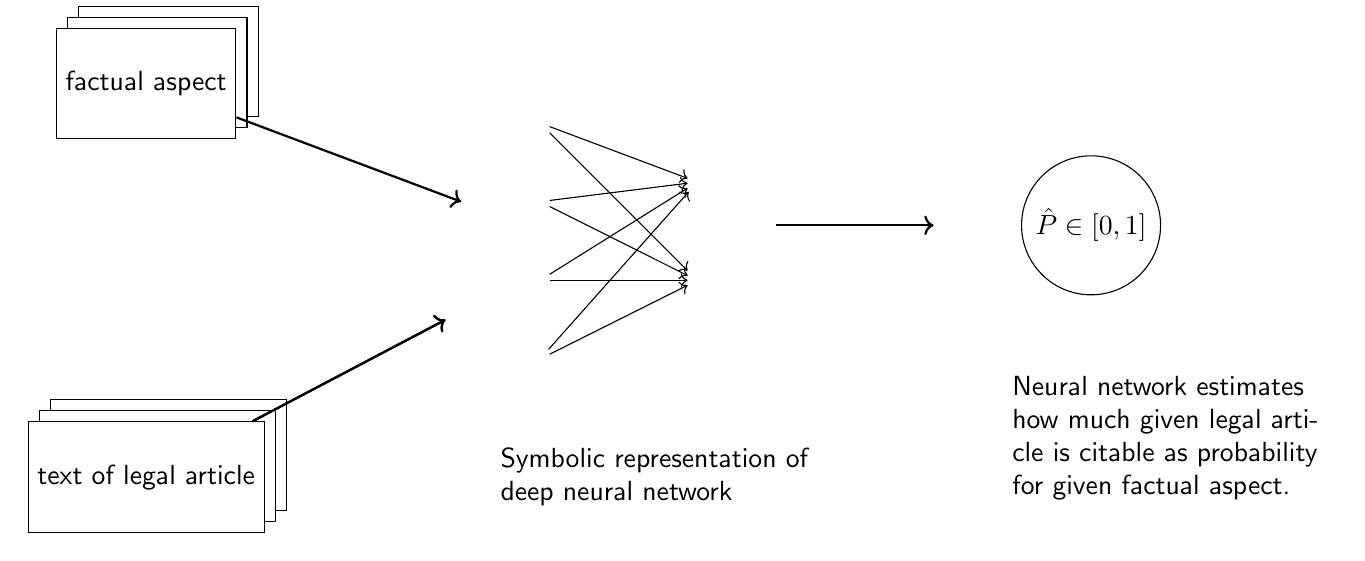
\begin{tikzpicture}[font=\sffamily,
            doc/.style={draw, minimum height=4em, minimum width=3em,
                    fill=white,
                    double copy shadow={shadow xshift=4pt,
                            shadow yshift=4pt, fill=white, draw}},
        ]
        \begin{scope}[xshift=-8cm, yshift=2cm]
            \node[doc] at (0, 0) (factual) {factual aspect};
            % \node[text width=4cm] at (0.5,-2.1)
            % {``\textbf{Dual Retail System} allows imported beef to be sold only in specialized store \ldots ''};

            \node[doc] at (0, -5)(legal-article) {text of legal article};
            % \node[text width=4cm] at (0.5,-7.2)
            % {``\textbf{Article I:1} \ldots members \textit{shall not} discriminate between two different members of WTO \ldots''};


            % human torso with head
            \begin{scope}[xshift=5cm, yshift=-2cm]
                \foreach \m/\l [count=\y] in {1,2,3,4}
                \node [every neuron/.try, neuron \m/.try] (input-\m) at (0,2.5-\y) {};

                \foreach \m [count=\y] in {1,2}
                \node [every neuron/.try, neuron \m/.try ] (hidden-\m) at (2,2-\y*1.25) {};

                % \foreach \m [count=\y] in {1}
                % \node [every neuron/.try, neuron \m/.try ] (output-\m) at (4,1.2-\y) {};

                \foreach \i in {1,...,4}
                \foreach \j in {1,...,2}
                \draw [->] (input-\i) -- (hidden-\j);

                % \foreach \i in {1,2}
                % \foreach \j in {1}
                % \draw [->] (hidden-\i) -- (output-\j);        
            \end{scope}
            \node[text width=4cm] at (6.5,-5)
            {Symbolic representation of deep neural network};


            % arrows to feed factual and article content
            \begin{scope}[every edge/.append style={->}] % for directed edge, change "style={->, double=black, draw=white}]"
                \path[->] (factual) edge[thick,->] node[above, xshift=5pt] {} +(4,-1.5);
                \path[->] (legal-article) edge[thick,->] node[above, xshift=10pt] {} +(3.8,2);
            \end{scope}

            \path[->] (legal-article) edge[thick,->] node[above, xshift=10pt] {} +(3.8,2);

            \draw[thick,->] (8,-1.8) -- (10,-1.8);
            \node [draw,circle] (P) at (12,-1.8){$\hat{P} \in [0,1]$ };
            \node[text width=4cm] at (13,-4.5)
            {Neural network estimates how much given legal article is citable as probability for given factual aspect.};


        \end{scope}
    \end{tikzpicture}
    \caption{\textbf{Design of Training Framework of Deep Neural Network:} I desgined a training framework of deep neural network by analogy with how member cites in WTO DSB as visualized in Figure \ref{fig:viz:how-member-cites-citable} and Figure \ref{fig:viz:how-member-cites-non-citable}.}
    \label{fig:design-of-nn}

\end{figure}

\begin{figure}[ht]
    \[\text{For given $V$, $D$ defined in Figure \ref{fig:set-of-articles-used} and  Figure \ref{fig:def:set-of-cited-articles},}\]
    \[\text{ let } E = \{e \mid e \text{ is an english word or special charcter} \} \text{ and }\]
    \[n_{\text{factual}}, n_{\text{article}} \in \Bbb N \text{ represents \textit{max token length} of factual aspect and legal article respectively}. \]
    
    \[\text{Then define } T = \{t_d \mid t_d = (e_1, e_2, \ldots , e_{n_\text{factual}}) \text{ } s.t. \text{ } d \in D \text{ and } e_{i \le{n_{\text{factual}}}  } \in E \} \]
    \[\text{ where } t_d \text{ represents a factual aspect of one of DS cases listed in Figure \ref{fig:ds-cases-used}. }\]
    
    \[\text{ Also, define } A = \{a_v \mid a_v = (e_1, e_2, \ldots , e_{n_\text{article}}) \text{ } s.t. \text{ } v \in V \text{ and } e_{i \le{n_{\text{article}}}  } \in E \}  \]
    \[\text{ where } a_v \text{ represents texts of one of the legal article listed in Figure \ref{fig:set-of-articles-used}. }\]

    \[\text{ Now defines a deep neural network } f \text{ with a set of parameters } \theta \]
    \[f_{\theta}: T \times A \to [0, 1] \]

    % set of factual aspects for all cases in Figure \ref{fig:ds-cases-used} } f \delta^d_{ij} \text{ is defined to be } 1 \text{ if } \{(v_i, v_j) \mid v_i, v_j \in V \text{ and } i \neq j \} \subset c_{d \in D} \ \text{ else } 0\]
    % \[\text{ where } V, D \text{ and } c_d \text{ is defined as in Figure \ref{fig:def:set-of-cited-articles}}. \]
    % \[\text{Then let \textit{co-citation matrix} } M = (m_{ij}) \in \Bbb{N}^{|V| \times |V|} \text{ s.t. } m_{ij} = \sum_{d \in D}\sum_{i,j \in V}\delta^d_{ij}\]

    \caption{\textbf{Formal Definition of Input/Output of Deep Neural Network}: $T$ and $A$ represents a set of ``documents" that are factual aspects and text of legal articles respectively. The term ``document" refer to a \textit{tuple} of English words or special characters like $(e_1, e_2, \ldots, e_{n_\text{max}})$. Then a pair of two documents, factual aspect and legal article, is fed into the neural network $f$ and returns a probability that represents how much the given article is citable for the given factual aspect.}
    \label{fig:def:io:nn}

\end{figure}

\subsubsection{Structure of Deep Neural Network} 
\subsubsection{Train of Deep Neural Network} 


% \subsubsection{Embedding Layer}
\begin{figure}[h]
    \centering
    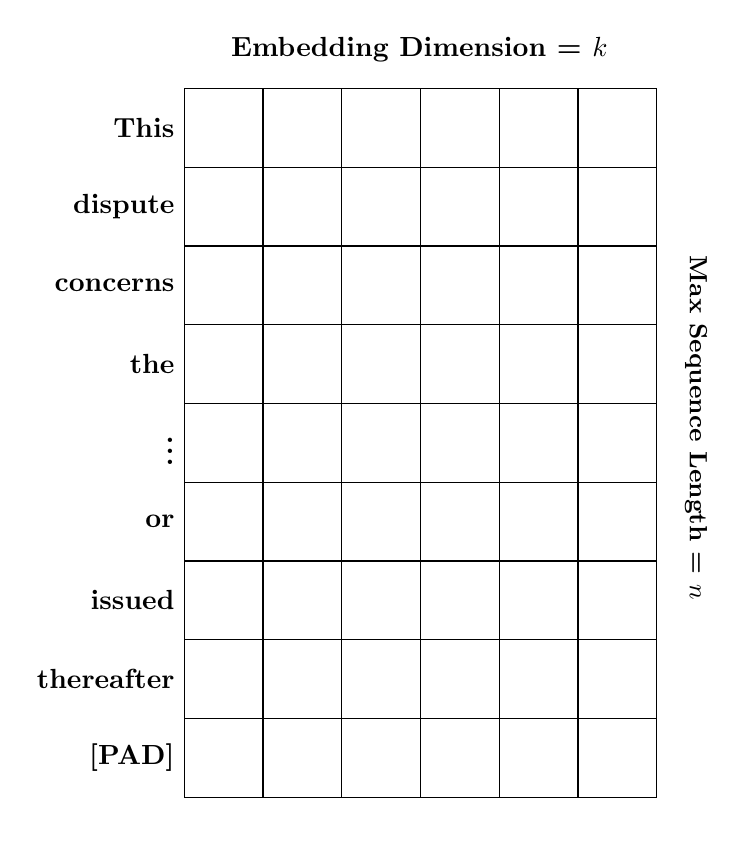
\begin{tikzpicture}
        \foreach \i in {\xMin,...,\xMax} {
            \draw [black] (\i,\yMin) -- (\i,\yMax) node [below] at (\i,\yMin) {};
        }
        \foreach \i in {\yMin,...,\yMax} {
            \draw [black] (\xMin,\i) -- (\xMax,\i) node [left] at (\xMin,\i) {};
        }

        \node [left] at (0,0.5) {\textbf{[PAD]}};
        \node [left] at (0,1.5) {\textbf{thereafter}};
        \node [left] at (0,2.5) {\textbf{issued}};
        \node [left] at (0,3.5) {\textbf{or}};
        \node [left] at (0,4.5) {\textbf{\vdots}};
        \node [left] at (0,5.5) {\textbf{the}};
        \node [left] at (0,6.5) {\textbf{concerns}};
        \node [left] at (0,7.5) {\textbf{dispute}};
        \node [left] at (0,8.5) {\textbf{This}};

        \node [left] at (5.5,9.5) {\textbf{Embedding Dimension = $k$}};
        \node [right, rotate=-90, font=\small] at (6.5,7) {\textbf{Max Sequence Length = $n$}};


    % \draw [step=1.0,blue, very thick] (0.5,0.5) grid (5.5,4.5);
    % \draw [very thick, brown, step=1.0cm,xshift=-0.5cm, yshift=-0.5cm] (0.5,0.5) grid +(5.5,4.5);
    \end{tikzpicture} 
    \label{fig:embedding}      
    \caption{\textbf{Embedding Layer:} $n \times k$ matrix representation of factual aspect} 
\end{figure}

% This  dispute  concerns  the  Continued  Dumping 

% \subsubsection{1-Dimensional Convolution Layer (Conv1D)}
\begin{figure}[h]
    \centering
    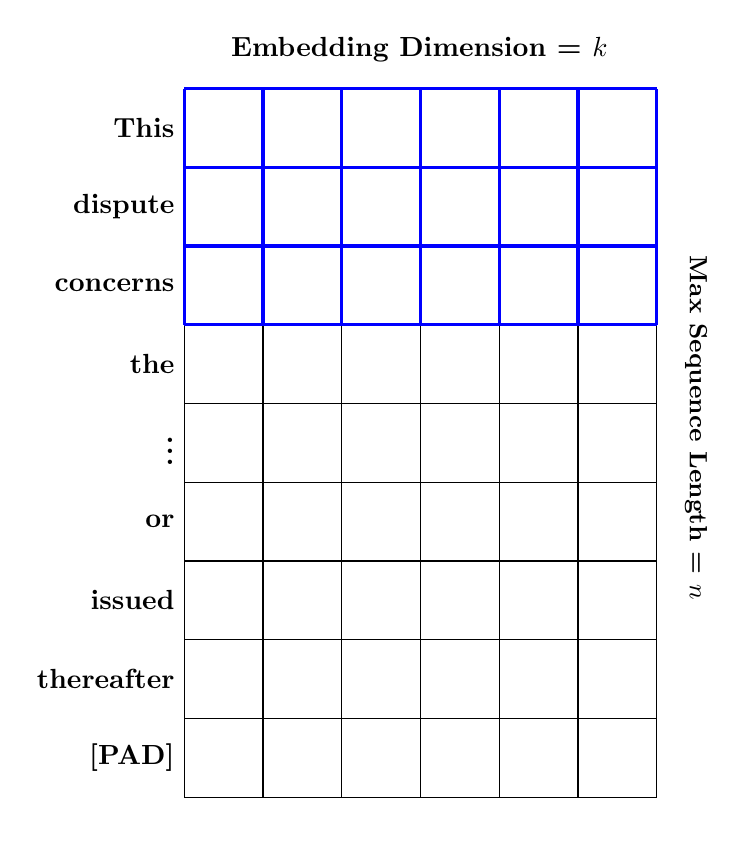
\begin{tikzpicture}
        \foreach \i in {\xMin,...,\xMax} {
            \draw [black] (\i,\yMin) -- (\i,\yMax) node [below] at (\i,\yMin) {};
        }
        \foreach \i in {\yMin,...,\yMax} {
            \draw [black] (\xMin,\i) -- (\xMax,\i) node [left] at (\xMin,\i) {};
        }

        \node [left] at (0,0.5) {\textbf{[PAD]}};
        \node [left] at (0,1.5) {\textbf{thereafter}};
        \node [left] at (0,2.5) {\textbf{issued}};
        \node [left] at (0,3.5) {\textbf{or}};
        \node [left] at (0,4.5) {\textbf{\vdots}};
        \node [left] at (0,5.5) {\textbf{the}};
        \node [left] at (0,6.5) {\textbf{concerns}};
        \node [left] at (0,7.5) {\textbf{dispute}};
        \node [left] at (0,8.5) {\textbf{This}};

        \node [left] at (5.5,9.5) {\textbf{Embedding Dimension = $k$}};
        \node [right, rotate=-90, font=\small] at (6.5,7) {\textbf{Max Sequence Length = $n$}};


    \draw [step=1.0,blue, very thick] (0,9) grid (6,6); % 3-filter

    % \draw [step=1.0,red, very thick] (0,5) grid (6,1); % 3-filter

    % \draw [very thick, brown, step=1.0cm,xshift=-0.5cm, yshift=-0.5cm] (0.5,0.5) grid +(5.5,4.5);
    \end{tikzpicture} 
    \label{fig:conv1d}      
    \caption{\textbf{Embedding Layer:} $n \times k$ matrix representation of factual aspect} 
\end{figure}

% This  dispute  concerns  the  Continued  Dumping 

% \subsubsection{1-Dimensional Max-pooling (MaxPool1D)}
\begin{figure}[h]
    \centering
    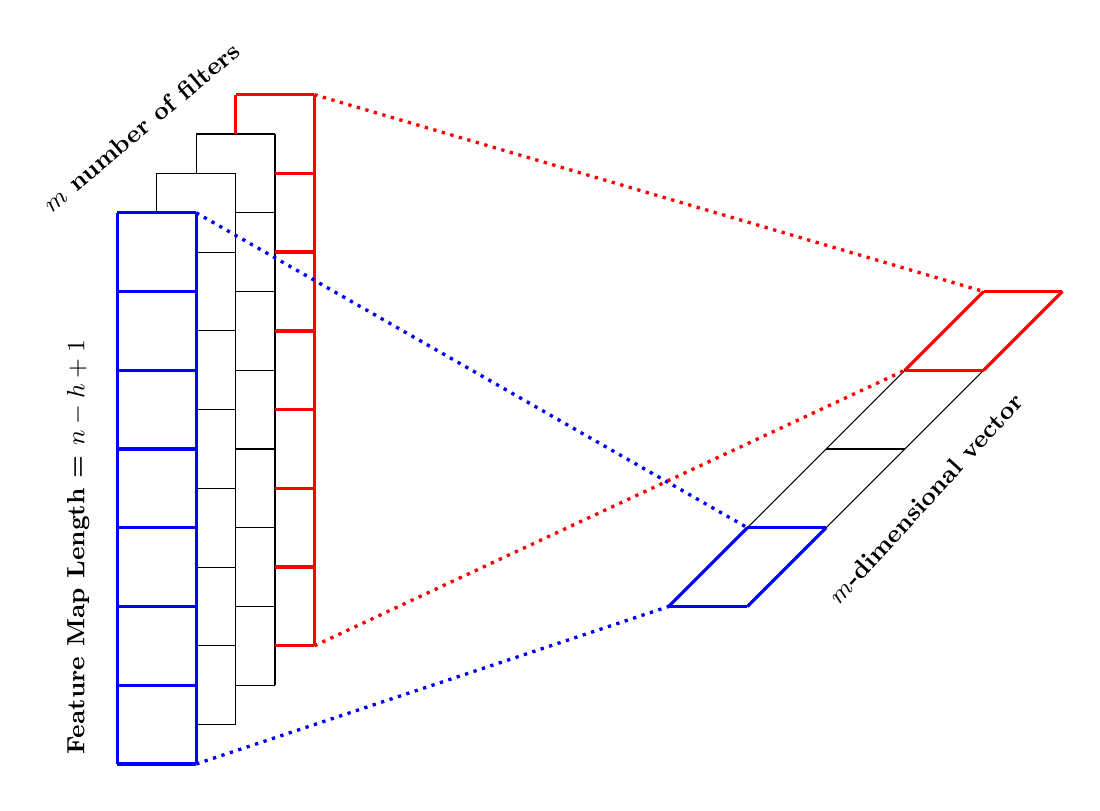
\begin{tikzpicture}
    % Conv Runs Output-0
    \foreach \i in {0,...,1} {
        \draw [black] (\i,\yMinOut) -- (\i,\yMaxOut) node [below] at (\i,\yMinOut) {};
    }
    \foreach \i in {\yMinOut,...,\yMaxOut} {
        \draw [black] (0,\i) -- (1,\i) node [left] at (0,\i) {};
    }
    % Conv Runs Output-1
    \draw [black] (1.5,\yMinOut+0.5) -- (1.5,\yMaxOut+0.5) node [below] at (1.5,\yMinOut+0.5) {};
    \foreach \i in {\yMinOut,...,\yMaxOut} {
        \draw [black] (1,\i+0.5) -- (1.5,\i+0.5) node [left] at (0,\i+0.5) {};
    }
    \draw [black] (0.5,\yMaxOut+0.5) -- (1,\yMaxOut+0.5) node [left] at (0,\yMaxOut+0.5) {};
    \draw [black] (0.5,\yMaxOut) -- (0.5,\yMaxOut+0.5) node [below] at (0.5,\yMinOut+0.5) {};
    
    % Conv Runs Output-2
    \draw [black] (2,\yMinOut+1) -- (2,\yMaxOut+1) node [below] at (2,\yMinOut+1) {};
    \foreach \i in {\yMinOut,...,\yMaxOut} {
        \draw [black] (1.5,\i+1) -- (2,\i+1) node [left] {};
    }
    \draw [black] (1,\yMaxOut+1) -- (1.5,\yMaxOut+1) node [left] {};
    \draw [black] (1,\yMaxOut+0.5) -- (1,\yMaxOut+1) node [below] {};

    % Conv Runs Output-2
    \draw [black] (2,\yMinOut+1) -- (2,\yMaxOut+1) node [below] at (2,\yMinOut+1) {};
    \foreach \i in {\yMinOut,...,\yMaxOut} {
        \draw [black] (1.5,\i+1) -- (2,\i+1) node [left] {};
    }
    \draw [black] (1,\yMaxOut+1) -- (1.5,\yMaxOut+1) node [left] {};
    \draw [black] (1,\yMaxOut+0.5) -- (1,\yMaxOut+1) node [below] {};
    
    % Conv Runs Output-3
    \draw [red, very thick] (2.5,\yMinOut+1.5) -- (2.5,\yMaxOut+1.5) node [below] {};
    \foreach \i in {\yMinOut,...,\yMaxOut} {
        \draw [red, very thick] (2,\i+1.5) -- (2.5,\i+1.5) node [left] {};
    }
    \draw [red, very thick] (1.5,\yMaxOut+1.5) -- (2,\yMaxOut+1.5) node [left] {};
    \draw [red, very thick] (1.5,\yMaxOut+1) -- (1.5,\yMaxOut+1.5) node [below] {};
    
    %Axis ticks
    \node [right, rotate=90, font=\small] at (-0.5,1) {\textbf{Feature Map Length = $n-h+1$}};
    \node [right, rotate=40, font=\small] at (-1,8) {\textbf{$m$ number of filters}};
    \node [right, rotate=47.5, font=\small] at (9,3) {\textbf{$m$-dimensional vector }};

    %Max Pool Output
    \draw [black] (7,3) -- (11,7) node [below] {};
    \draw [black] (8,3) -- (12,7) node [below] {};

    \foreach \i in {3,...,7} {
        \draw [black] (\i+4,\i) -- (\i+5,\i) node [left] {};
    }
    
    %Blue on Output
    \draw [blue, very thick] (7,3) -- (8,3) node [left] {};
    \draw [blue, very thick] (8,4) -- (9,4) node [left] {};
    \draw [blue, very thick] (7,3) -- (8,4) node [below] {};
    \draw [blue, very thick] (8,3) -- (9,4) node [below] {};

    %Red on Output
    \draw [red, very thick] (10,6) -- (11,6) node [left] {};
    \draw [red, very thick] (11,7) -- (12,7) node [left] {};
    \draw [red, very thick] (10,6) -- (11,7) node [below] {};
    \draw [red, very thick] (11,6) -- (12,7) node [below] {};

    % Connection between Two Matrix
    \draw[dotted,blue, very thick] (1,8) -- (8,4);
    \draw[dotted,blue, very thick] (1,1) -- (7,3);

    \draw[dotted,red, very thick] (2.5,9.5) -- (11,7);
    \draw[dotted,red, very thick] (2.5,2.5) -- (10,6);
    
    % Grid 
    \draw [step=1.0,blue, very thick] (0,8) grid (1,1); % 3-filter

    \end{tikzpicture} 

    
    % \caption{\textbf{Conv1D:} $m$ number of $h$-sized filter runs over the $n \times k $ embedding matrix and produces $m \times (n-h+1)$ matrix}
    \caption{\textbf{MaxPool1D:} Filter out max value for all $m$ number of feature map outputs from $m$ different convolution filters. MaxPool1D produces a $m$ dimensional vector as an output for collection of those filtered max values.} % actually feature map means "after" non-linear activation.
    \label{fig:maxpool1d}      

\end{figure}

% This  dispute  concerns  the  Continued  Dumping 

% \subsection{Reconstruction of Network of Articles of WTO Agreements}
\subsection{Fitting $G^* = (V, E, W^*)$ Using Ensemble of Random Forests}
\subsubsection{Definition of $W^*$: Best Set of Directed Edge Weights} %for the Network of Legal Articles of the WTO agreements}
Let $f_{\theta^*}$ represent the trained neural network with an optimized set of parameters $\theta^*$. 
Then we can construct a prediction matrix $P = (f_{\theta^*}(t_d, a_v)) \in [0,1]^{{|D| \times |V|}}$  by collecting all predictions $f_{\theta^*}(t_d, a_v)$ from the trained neural network $f_{\theta^{*}}$ using the all pairs of data $(t_d,a_v) \in T \times A$ as illustrated in Figure \ref{fig:illutrate-preds}.

Upon the assumption that the trained neural network $f_{\theta^*}$ effectively encodes a shared understanding among legal experts of WTO agreements, our task is to find a set of directed edge weights $W^* = \{w^{*}_{ij} \mid w^{*}_{ij} = w^{*}(v_i, v_j) \text{ } s.t. \text{ } w(v_j, v_j)^{*} = 0 \text{ and } \sum_{v_i\in V}{w^{*}(v_i, v_j)} = 1 \text{ } \forall v_j \}$ %W^* = w(v_i, v_j)$ where
by exploiting the information inside the prediction matrix $P = (f_{\theta^*}(t_d, a_v)) \in [0,1]^{{|D| \times |V|}}$. This set of directed edge weights $W^{*} = \{w^{*}_{ij}\}$ shall represent a set of conditional praobability $P^{*}(v_j|v_i)$ how probably a source node $v_i$ clarifies the meaning of the target node $v_j$ compared to other source nodes
as closely as to a shared understanding of legal experts of WTO agreements.

To perform this task, this paper adopts a machine learning technique called \textit{Random Forest (RF)} that can rank input variables in terms of relative importance to explain the variance of output variable. The step-by-step algorithm of \textit{Random Forest} will be explained in the next subsection.

% as illustrated in Figure \ref{fig:def-example}.
% This paper defines $W^*$ as a set of directed edge weights that best explains the co-citation pattern inside the prdiction matrix $P = (f_{\theta^*}(t_d, a_v)) \in [0,1]^{{|D| \times |V|}}$.  % that is visualized in Figure \ref{predidction_matrix}.

% To numerically ``best explains'' is that for given 


% == HEATMAP MATRIX == 
\begin{figure}[!tbp]
  \begin{subfigure}[b]{0.49\textwidth}
    \centering
    \resizebox{\columnwidth}{!}{
      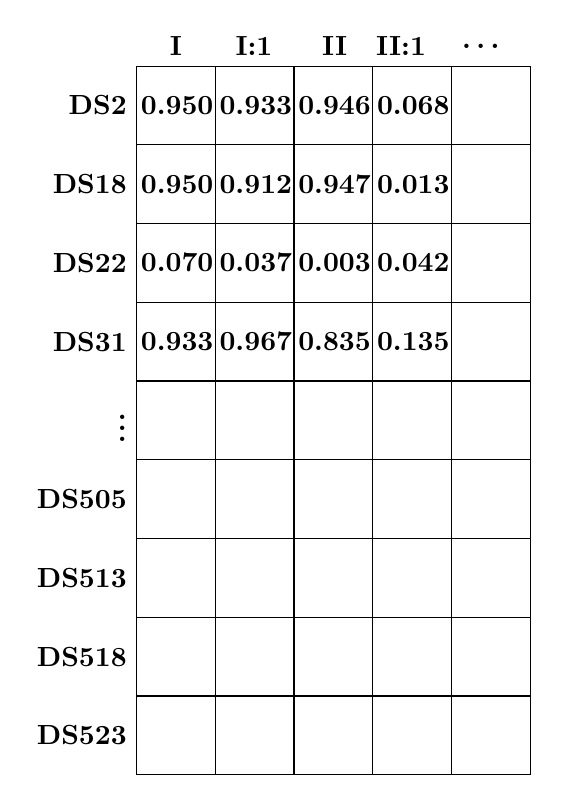
\begin{tikzpicture}
        \foreach \i in {\xMin,...,5} {
            \draw [black] (\i,0) -- (\i,9) node [below] at (\i,4) {};
          }
        \foreach \i in {0,...,9} {
            \draw [black] (\xMin,\i) -- (5,\i) node [left] at (\xMin,\i) {};
          }
        \node [left] at (0,0.5) {\textbf{DS523}};
        \node [left] at (0,1.5) {\textbf{DS518}};
        \node [left] at (0,2.5) {\textbf{DS513}};
        \node [left] at (0,3.5) {\textbf{DS505}};
        % \node [left] at (0,4.5) {\textbf{DS4}};
        % \node [left] at (0,5.5) {\textbf{DS4}};
        \node [left] at (0,4.5) {\textbf{\vdots}};
        \node [left] at (0,5.5) {\textbf{DS31}};
        \node [left] at (0,6.5) {\textbf{DS22}};
        \node [left] at (0,7.5) {\textbf{DS18}};
        \node [left] at (0,8.5) {\textbf{DS2}};

        \node [left] at (4.8, 9.25) {\textbf{\ldots}};
        \node [left] at (3.8, 9.25) {\textbf{II:1}};
        \node [left] at (2.8, 9.25) {\textbf{II}};
        \node [left] at (1.85, 9.25) {\textbf{I:1}};
        \node [left] at (0.7,9.25) {\textbf{I}};

        \node [left] at (1.1,8.5) {\textbf{0.950}};
        \node [left] at (2.1,8.5) {\textbf{0.933}};
        \node [left] at (3.1,8.5) {\textbf{0.946}};
        \node [left] at (4.1,8.5) {\textbf{0.068}};

        \node [left] at (1.1,7.5) {\textbf{0.950}};
        \node [left] at (2.1,7.5) {\textbf{0.912}};
        \node [left] at (3.1,7.5) {\textbf{0.947}};
        \node [left] at (4.1,7.5) {\textbf{0.013}};

        \node [left] at (1.1,6.5) {\textbf{0.070}};
        \node [left] at (2.1,6.5) {\textbf{0.037}};
        \node [left] at (3.1,6.5) {\textbf{0.003}};
        \node [left] at (4.1,6.5) {\textbf{0.042}};

        \node [left] at (1.1,5.5) {\textbf{0.933}};
        \node [left] at (2.1,5.5) {\textbf{0.967}};
        \node [left] at (3.1,5.5) {\textbf{0.835}};
        \node [left] at (4.1,5.5) {\textbf{0.135}};

      \end{tikzpicture}
    }
    \label{fig:illutrate-preds}
    \caption{\textbf{Illustration of Prediction Matrix:} By defining row as a list of DS case numbers and column as legal articles, we can create $|D| \times |V|$ matrix that includes $f_{\theta^*}(t_d, a_v)$ for each cell.}
  \end{subfigure}
  \hfill
  \begin{subfigure}[b]{0.49\textwidth}
    \centering{
      \resizebox{\textwidth*\real{\heatmap}}{\textwidth*\real{\heatmap} * \real{1.7889}}{
        % This file was created by tikzplotlib v0.9.4.
\begin{tikzpicture}

\begin{axis}[
hide x axis,
hide y axis,
tick align=outside,
tick pos=left,
x grid style={white!69.0196078431373!black},
xmin=0, xmax=80,
xtick style={color=black},
y grid style={white!69.0196078431373!black},
ymin=0, ymax=143,
ytick style={color=black}
]
\addplot graphics [includegraphics cmd=\pgfimage,xmin=0, xmax=80, ymin=0, ymax=143] {pred_only.png};
\end{axis}

\end{tikzpicture}

      }
      \resizebox{\columnwidth}{!}{
        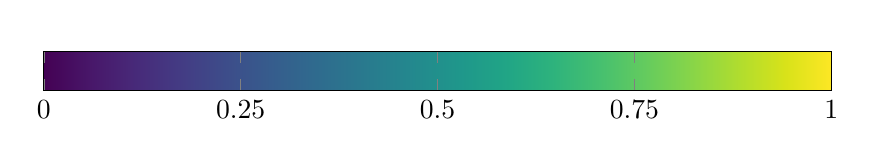
\begin{tikzpicture}
          \begin{axis}[
              hide axis,
              scale only axis,
              height=0pt,
              width=0pt,
              colormap/viridis,
              colorbar horizontal,
              point meta min=0,
              point meta max=1,
              colorbar style={
                  width=10cm,
                  height=0.5cm,
                  xtick={0,0.25,0.5,0.75,1}
                }]
            \addplot [draw=none] coordinates {(0,0)};
          \end{axis}
        \end{tikzpicture}
      }

      \caption{\textbf{Prediction Matrix:} This heatmap represents the $P$ from the actual data and its predictions from $f_{\theta^*}$}
      \label{predidction_matrix}
    }
  \end{subfigure}
  \caption{\textbf{Illustration of Prediction Matrix:} I collected all the predictions from the trained neural network $f_{\theta^*}$ and constructed prediction matrix $P$}
  \label{fig:illutrate-preds}
\end{figure}


% \[w : V \times V \to \Bbb R_{+} \text{ } s.t. \text{ } w(v_i, v_i) = 0 \text{ and } \sum_{v_i\in V}{w(v_i, v_j)} = 1 \text{  } \forall v_i, v_j \in V \] %\text{ and }\]


\subsubsection{Random Forest on Prediction Matrix: Finding $W^*$} %for the Network of Legal Articles of the WTO agreements}
\clearpage
\begin{algorithm}[H]
    \DontPrintSemicolon

    \KwInput{Prediction Matrix $P = (p_{dv}) \in [0,1]^{{|D| \times |V|}} \text{ s.t. } p_{dv} = f_{\theta^*}(t_d, a_v)$}
    \KwOutput{$W^* = (w^*_{ij}) \in [0,1]^{|V| \times |V|}$}
    Let number of features $n = |V|$ , \\
    $\:\:\:\:\:\:\:$ number of obseravations $o = |D|$ and \\
    $\:\:\:\:\:\:\:$ number of trees to ensemble $ m \in \Bbb N$

    \For{$v_j \in V $} {
        X $\gets \{ x_d \mid x_d = (p_{dv_1},\: p_{dv_2},\: \ldots, \:p_{dv_{n}}) \: s.t. \: v \in V \setminus{\{v_j\}} \text{ and } d \in D \} \:$  \\
        Y $\gets \{ y_d  \mid y_d = p_{dv_j} \: / \sigma(p_{v_j}) \: s.t. \: d \in D \text{ and } \sigma(p_{v_j}) \text{ is a standard deviation of }$ \\
        $\{ p_{dv_j} \mid d \in D \} \}$\\

        \For{$ k \in \{1,2, \ldots, m \} $} {
            1. $S = \{(x_d, y_d)\} \gets $ Random sample $o$ number of $(x_d, y_d)$ from $X \times Y$ with replacement. Then let $X_d$ notate set of all sampled $x_d$. \\
            2. Find a decision tree $T_k: X_d \to \Bbb R$ where\\
            $T_k = \{ N \mid N = (v_i, b, N_p, \hat{y}) $ represents a decision node where \\ 
            $ b, \hat{y} \in \Bbb R, v_i \in V \setminus{\{v_j\}} $ and $(v_i, b) \text{ splits } S_N \subset S \text{ that reached the node } N $\\
            into $S_{N_{true}}$ and $S_{N_{false}}$ with a criterion $p_{dv_i} \ge b$ with a parent node $ N_p \in T_k$ \\             if $N$ is not a root node. Define $N_p = \emptyset$ if N is a root node. $\hat{y}$ represents \\
            the node's estimate for given input. $v_i$ and $b$ is $\emptyset$ if $N$ has no child node(s).$\}$\\
            that minimizes the MSE loss $\sum_{(x_d, y_d) \in S} \frac{1}{|S|}(y_d - T_k(x_d))^2$.\\
            3.
            \For{$N \in T_i$ } {
                \If{$v_i$ of $N \neq \emptyset$ }
                {
                    % $I(N) \gets \frac{1}{|S|^2}\sum_{i \in S}\sum_{j \in S}$
                    $I^k_{v_i \to v_j}(N) \gets \text{Var}(S_N) - \text{Var}(S_{N_{true}}) - \text{Var}(S_{N_{false}})$ where Var($\cdot$) is the variance
                    of the output variable $y_d$ in each subset $S_N, S_{N_{true}}$ and $S_{N_{false}}$           
                } 

            }
    
        }
    }
    \text{\textbf{then}} $w^*_{ij} \gets \frac{1}{m}\sum_{k \in \{ 1, 2, ... m\}} I^k_{v_i \to v_j}(N)$ \\
    \text{\textbf{return}} $W^* = (w^*_{ij}) \in [0,1]^{|V| \times |V|}$
    % \KwData{Testing set $x$}
    % $\sum_{i=1}^{\infty} := 0$ \tcp*{this is a comment}
    % \tcc{Now this is an if...else conditional loop}
    % \If{Condition 1}
    % {
    %     Do something    \tcp*{this is another comment}
    %     \If{sub-Condition}
    %     {Do a lot}
    % }
    % \ElseIf{Condition 2}
    % {
    %     Do Otherwise \;
    %     \tcc{Now this is a for loop}
    %     \For{sequence}
    %     {
    %         loop instructions
    %     }
    % }
    % \Else
    % {
    %     Do the rest
    % }

    % \tcc{Now this is a While loop}
    % \While{Condition}
    % {
    %     Do something\;
    % }

    \caption{Random Forest To Find $W^*$}
\end{algorithm}

\section{Empirical Findings} %: Quality Check of the Fitted Network $G^*$}
This section verifies
how well the fitted network $G^* = (V, E, W^*)$
aligns with the jurisprudence of the \textit{Panel} or \textit{Appellate Body} of WTO DSB.
Since these two judicial bodies of WTO DSB authoritatively
opinionate how the regulatory system of WTO DSB systemetically organized,
this paper will validate the quality of the fitted network $G^*$ by 
introducing three different sub-networks of 
the fitted network $G^*$ where each sub-network shows how different articles of WTO agreements 
cooperatively achieves a important principle of WTO 
at the following subsections.





\subsection{\textit{Market Access}: Ensuring Foreign Goods to Cross Borders and Fairly Compete with Domestic Products}

% == THREE SUBSYSTEM == 
\begin{figure}[ht]
    \centering{
        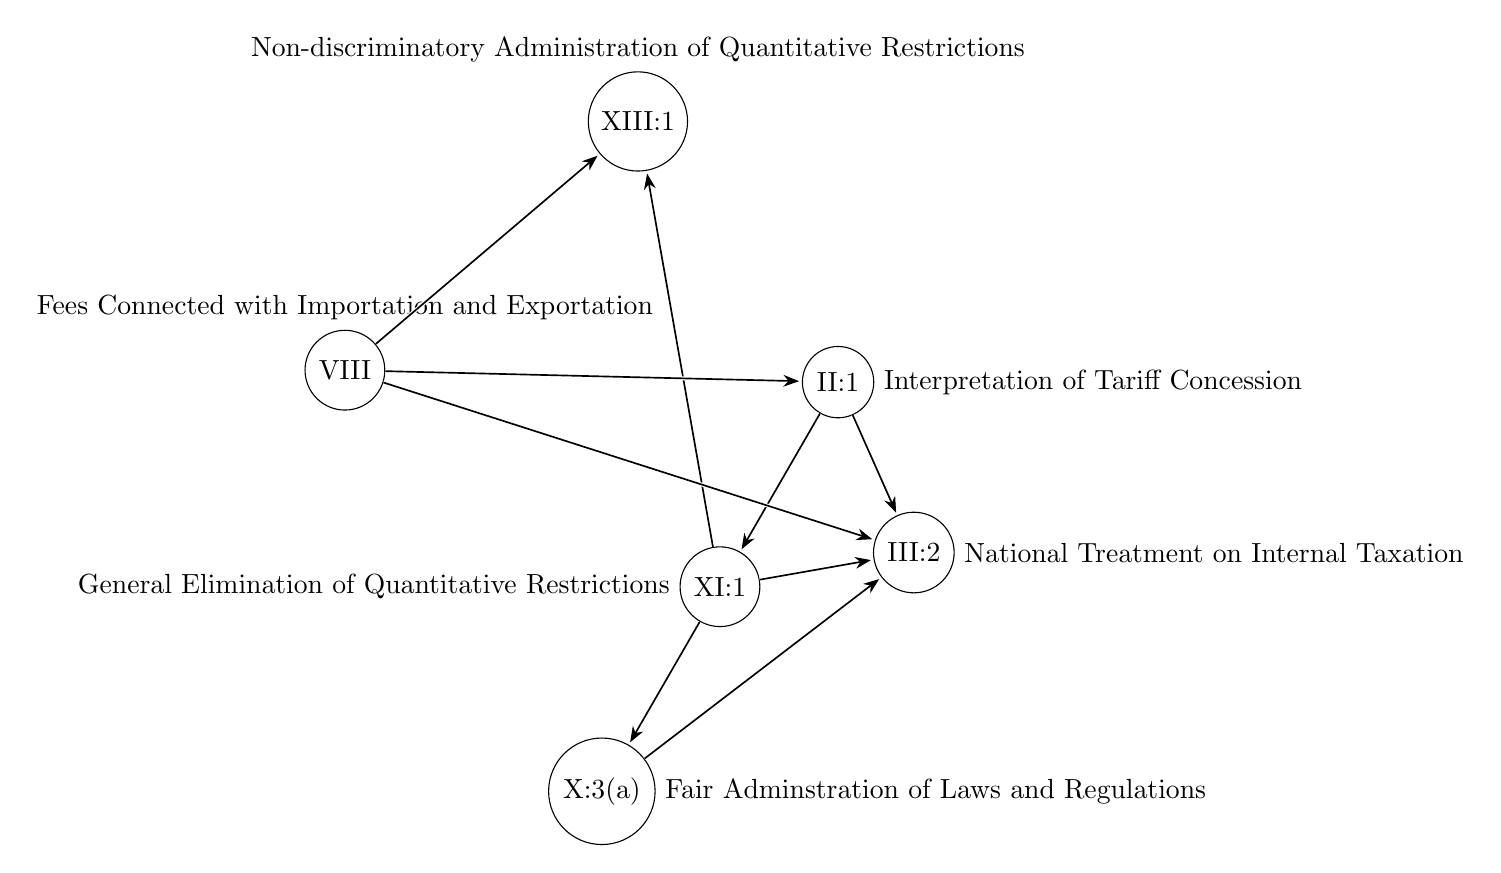
\begin{tikzpicture}[>={Stealth[color=black]},shorten >=1pt,node distance=2cm,on grid,initial/.style={}]
  \node[state, label=right:Interpretation of Tariff Concession] (T1) {II:1};
  \node[state, label=left:General Elimination of Quantitative Restrictions] at ([shift=({240:3 cm})]T1) (T4) {XI:1};
  \node[state, label=right:Fair Adminstration of Laws and Regulations] at ([shift=({240:3 cm})]T4) (T5) {X:3(a)};
  \node[state, label=above:Non-discriminatory Administration of Quantitative Restrictions] at ([shift=({100:6 cm})]T4) (T7) {XIII:1};
  \node[state, label=right:National Treatment on Internal Taxation] at ([shift=({10:2.5 cm})]T4) (T6) {III:2};
  \node[state, label=above:Fees Connected with Importation and Exportation] at ([shift=({150:5.5 cm})]T4) (T8) {VIII};

  \begin{scope}[every edge/.append style={->, double=black, draw=white}] % for directed edge, change "style={->, double=black, draw=white}]"
    \path (T1)
    edge   (T4)
    edge   (T6);
    \path (T4)
    edge   (T5)
    edge   (T6)
    edge   (T7);
    \path (T5)
    edge   (T6);
    \path (T8)
    edge   (T7)
    edge   (T1)
    edge   (T6);

  \end{scope}
\end{tikzpicture}

% to draw the node's border w/ color, refer to https://tex.stackexchange.com/questions/438412/how-to-add-border-to-a-node
    }
    \caption{{\bf Network of the Articles that Achieves \textit{Market Access}:}
        This figure demonstrates a network of articles of WTO agreements
        that cooperatively achieves the principle of \textit{Market Access} in the regulatory system of WTO.
        Tariff and Non-tariff barriers such as quantitative restriction, internal taxations
        and extra fees for crossing border can inhibit the chance of foreign goods to access the foreign market.
        Therefore, these articles tend to work together to ensure the \textit{Market Access} principle working properly.
        %(Directions and weights of network edges are omitted for brevity.)
    }
    \label{fig:market-aceess_directed}
  \end{figure}
  
% Figure \ref{fig:market-aceess_directed} shows a part of the fitted network $G^*$ that explains how
% the articles of WTO agreements are interconnected each other to acheive one of the main principles of 
% WTO, \textit{Market Access}. 
\textit{Market Access} 
refers to the guarantee of the conditions relating to the 
tariff or non-tariff measures 
for the entry of 
goods into the foreign market. For example, if 
a country set a limit on the quantity of imported goods, no foreign goods above that limit can get access to that market. Also, if a country set a high tariff rate for a imported goods to cross the border, 
it also prevents foreign goods from accessing to that market.
Therefore, \textit{Market Access} is the most basic but important principle of the WTO
because it directly represent the primary goal of the WTO, smoothing the world trade flow.

Three different types of measures - quantitative restriction, tariff and internal taxation or regulations - are recocgnized as 
three major types of measures that protectionistic country prefer to use. For example, a country can
discriminate imported and domestic product with internal regulation such as enforcing the specialized retail channel for the imported product as \textit{Korea - Beef} case as introduced in section \ref{subsec:design:dnn}.
This discrimination provide a unfair ground of competition between domestic and imported products and it can eventually exclude imported beef from the Korean beef market.
These three main types of measures that are relevant to the \textit{Market Access} is illustrated in Figure \ref{fig:market-aceess_directed}.
Article XI:1, II:1 and III correponds to the obligations that regulates quantitative restriction, tariff and internal taxation respectively.
Edges are colored in red if the mean of the two directed edge weights are greater than $10\%$. For example, $w^*(\text{II:1}, \text{III}) = 0.117$ and $w^*(\text{III}, \text{II:1}) = 0.122$ thus their simple mean is 11.95\% which is greater than 10\%.
This red triangle that is comprised of Article XI:1, II:1 and III shows that the fitted network $G^* = (V, E, W^*)$ captures the principle of \textit{Market Access} as a cluster of articles with large edge weights. Moreover, 
the fitted network $G^*$ also captures sub-articles that supports this \textit{Market Access} triangle. For example, I colored edges in blue if the mean of the two directed edge weights are greather than 5\% and less than 10\%.
The Article X:3(a) which prohibits a unfair adminstration of laws and regulations are connected to the Article XI:1 and III that are mostly 
deteriorates the principle of \textit{Market Access} by unfair adminstration of laws and regulations relating to the quantitative restriction 
and competitive relationship between imported and domestic products. Also, in a similar notion, Article VIII get connected to the Article II:1 because 
often the fees connected with the importation are charged with huge amount and can deteriorates the principle of \textit{Market Access} as well.

% Mean of directive edge weights between Article II:1, III and XI:1 are $0.289$, 



% having a sum of directive edge weights bigger than 0.15, which is about ten times bigger than that of  

% The three major articles of the WTO agreements 
% that regulates 


\subsection{\textit{Reciprocity} in Non-Tariff Barriers: Compensate or Retaliate as Much as You have Protected}
% \subsection{\textit{Non-Tariff Barriers}: Anti-dumping, Countervailing Duties and Safeguard}
\begin{figure}[h]
    \centering{
        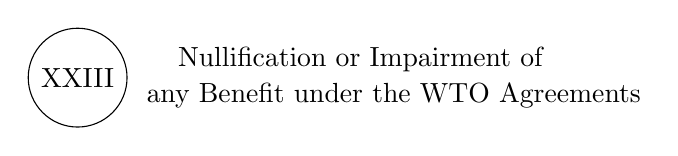
\begin{tikzpicture}[
  >={Stealth[color=black]}
  ,shorten >=1pt,node distance=2cm
  ,on grid,initial/.style={}
  ,every label/.style={align=left}
]

  \linespread{2} % to adjust the line spacing inside the label

  \node[state, label=right:{ \hspace{4mm} Nullification or Impairment of \\[1mm] \hspace{0mm} any Benefit under the WTO Agreements}] (T1) {XXIII};

  % \node[state, label=right:{Interpretation of \\[1mm] \hspace{-1mm} Tariff Concession}] (T1) {II:1};
  % \node[state, label=left:{General Elimination of \\[1mm] \hspace{-3mm} Quantitative Restrictions}] at ([shift=({240:3 cm})]T1) (T4) {XI:1};
  % \node[state, label=right:{Fair Adminstration of \\[1mm] \hspace{-1mm} Laws and Regulations}] at ([shift=({240:3 cm})]T4) (T5) {X:3(a)};
  % \node[state, label=above:{Non-discriminatory Administration of \\[1mm] \hspace{10mm} Quantitative Restrictions}] at ([shift=({100:6 cm})]T4) (T7) {XIII:1};
  % \node[state, label=right:{National Treatment on \\[1mm] \hspace{3mm} Internal Taxation}] at ([shift=({10:2.5 cm})]T4) (T6) {III:2};
  % % \node[state, label=above:Fees Connected with Importation and Exportation] at ([shift=({150:5.5 cm})]T4) (T8) {VIII};
  % % \node[state, label=right:{National Treatment on \\[1mm] \hspace{2mm} Internal Taxation}] at ([shift=({0:5 cm})]T1) (T2) {$v_j$ = III:2};
  % \node[state, label=left:{Fees Connected with \\[1mm] \hspace{-10mm} Importation and Exportation}] at ([shift=({150:5.5 cm})]T4) (T8) {VIII};


  % \begin{scope}[every edge/.append style={-, double=black, draw=white}] % for directed edge, change "style={->, double=black, draw=white}]"
  %   \path (T1)
  %   edge   (T4)
  %   edge   (T6);
  %   \path (T4)
  %   edge   (T5)
  %   edge   (T6)
  %   edge   (T7);
  %   \path (T5)
  %   edge   (T6);
  %   \path (T8)
  %   edge   (T7)
  %   edge   (T1)
  %   edge   (T6);

  % \end{scope}
\end{tikzpicture}

% to draw the node's border w/ color, refer to https://tex.stackexchange.com/questions/438412/how-to-add-border-to-a-node
    }
    \caption{{\bf Network of Articles that Achieves \textit{Reciprocity} for Non-Tariff Barriers:}
        This figure demonstrates a network of articles of WTO agreements
        that cooperatively regulates \textit{Non-Tariff Barriers} (NTBs) in WTO DSB.
        Three major NTBs such as \textit{Anti-dumping (AD)}, \textit{Countervailing Duties (CVD)}
        and \textit{Safeguard (SG)} are relying on the Article XXIII to resolve its inconsistency with the principle of \textit{Reciprocity}.
        %(Directions and weights of network edges are omitted for brevity.)
    }
    \label{fig:ntb-explained}
\end{figure}

Ensuring the \textit{Market Access} principle 
% by enforcing
% the binding tariff to imported products, by preventing the internal regulations from discrimintating the domestic and imported products
% and by eliminating the quantitative restrictions
is a basic approach to smooth the world trade flow as explained in the previous section. %subsection \ref{emp:ma}. 
However, members are sometimes allowed to apply higher duties or to maintain a quantitative restrictions in certain circumstances, such as 
to act against low-price dumping of foreign producers, to offset the distorted competitive realtionship resulted by the illegal subsidies
or to take an emergency measure in case irrevisible injury to domestic industry is expected. Each of these examples 
are called \textit{Anti-dumping (AD)}, \textit{Countervailing Duties (CVD)} and \textit{Safeguard (SG)} respectively. These measures are recognized as 
three major types of \textit{Non-Tariff Barriers} (NTBs) %that can easily constitue illegal trade barriers
since these three measures often fail to satisfy the legal requirements of the WTO agreements and evolve into trade dispute.

The principle of \textit{reciporocity} is a general notion that regulates these three major NTBs.
This principle requires change of value of imports affected by a country's trade policy 
shall be balanced with the equal value of exports across trading partners affected \citep{bagwell1999}.
The rules of the WTO agreements, in particular the Article XXIII of GATT 1994, 
confers a right to insist its nullfied or imparied benefit that is expected under the WTO agreements and require satisfactory adjustement to the member 
who results in such nullification or impariment. Moreover, this article confers a right to retaliate if no satisfatory adjustment being fulfilled.

Therefore, Article XXIII regulates this action-reaction characteristics of \textit{AD}, \textit{CVD} and \textit{SG} to achieve the priniple of \textit{reciprocity}. % as shown in Figure \ref{fig:ntb-explained}.
For example, \textit{Panel} stated that a member can resort to Article XXIII and raise a legal claim in case another member levies unjustified antidumping duties that fails to fully explain the causual realtionship between the dumping and the material injury to the related industry in its report on \textit{New Zealand - Imports of Eletrical Transformers from Finland}\footnote{\textit{WTO official document} L/5814, adopted on 18 July 1985, pp.67-68, para.4.4.}:

\begin{displayquote}[]
    ``Panel believed that if a contracting party
    affected by the determination (of levying \textbf{anti-dumping duties}) could make a case that the importation could not in itself have the effect of
    causing material injury to the industry in question, that contracting party was entitled, under the relevant
    GATT provisions, \textbf{in particular Article XXIII}, that its representations be given sympathetic consideration
    and that eventually, \textbf{if no satisfactory adjustment was effected, it might refer the matter to the CONTRACTING
    PARTIES\footnote{It means raising a legal claim through WTO DSB}}, as had been done by Finland in the present case."
\end{displayquote}

\noindent This realtionship is captured by the $6.3\%$ weight of directed edge from Article VI to Article XXIII. This is because citing Article VI (Antidumping duties and CVD) naturally leads to the citation of Article XXIII to insist its impaired benefit and solicit the satisfactory adjustment relying on the principle of \textit{reciprocity} in WTO DSB. 
Also, other two types of mesures, \textit{Illegal Subsidy} and \textit{SG} whose legal requirements are regulated under the Article XVI and XIX respectively also heavily rely ($>$ 10\%) on the Article XXIII to solicit its impaired benefit and satisfactory adjustment based on the principle of \textit{reciprocity} in case the breach of those requirments occurs. 

% Since these three types of measures 

\subsection{\textit{Rules of Formulating Free Trade Area} (FTA): No Higher Duties or more Restrictive regulation than Previous the corresponding duties and other regulations of}
% \subsection{\textit{Non-Tariff Barriers}: Anti-dumping, Countervailing Duties and Safeguard}
\begin{figure}[h]
    \centering{
        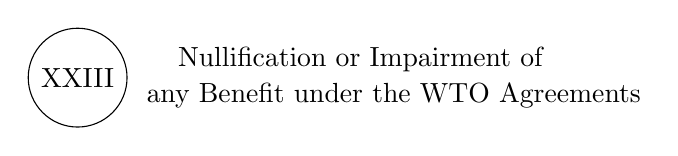
\begin{tikzpicture}[
  >={Stealth[color=black]}
  ,shorten >=1pt,node distance=2cm
  ,on grid,initial/.style={}
  ,every label/.style={align=left}
]

  \linespread{2} % to adjust the line spacing inside the label

  \node[state, label=right:{ \hspace{4mm} Nullification or Impairment of \\[1mm] \hspace{0mm} any Benefit under the WTO Agreements}] (T1) {XXIII};

  % \node[state, label=right:{Interpretation of \\[1mm] \hspace{-1mm} Tariff Concession}] (T1) {II:1};
  % \node[state, label=left:{General Elimination of \\[1mm] \hspace{-3mm} Quantitative Restrictions}] at ([shift=({240:3 cm})]T1) (T4) {XI:1};
  % \node[state, label=right:{Fair Adminstration of \\[1mm] \hspace{-1mm} Laws and Regulations}] at ([shift=({240:3 cm})]T4) (T5) {X:3(a)};
  % \node[state, label=above:{Non-discriminatory Administration of \\[1mm] \hspace{10mm} Quantitative Restrictions}] at ([shift=({100:6 cm})]T4) (T7) {XIII:1};
  % \node[state, label=right:{National Treatment on \\[1mm] \hspace{3mm} Internal Taxation}] at ([shift=({10:2.5 cm})]T4) (T6) {III:2};
  % % \node[state, label=above:Fees Connected with Importation and Exportation] at ([shift=({150:5.5 cm})]T4) (T8) {VIII};
  % % \node[state, label=right:{National Treatment on \\[1mm] \hspace{2mm} Internal Taxation}] at ([shift=({0:5 cm})]T1) (T2) {$v_j$ = III:2};
  % \node[state, label=left:{Fees Connected with \\[1mm] \hspace{-10mm} Importation and Exportation}] at ([shift=({150:5.5 cm})]T4) (T8) {VIII};


  % \begin{scope}[every edge/.append style={-, double=black, draw=white}] % for directed edge, change "style={->, double=black, draw=white}]"
  %   \path (T1)
  %   edge   (T4)
  %   edge   (T6);
  %   \path (T4)
  %   edge   (T5)
  %   edge   (T6)
  %   edge   (T7);
  %   \path (T5)
  %   edge   (T6);
  %   \path (T8)
  %   edge   (T7)
  %   edge   (T1)
  %   edge   (T6);

  % \end{scope}
\end{tikzpicture}

% to draw the node's border w/ color, refer to https://tex.stackexchange.com/questions/438412/how-to-add-border-to-a-node
    }
    \caption{{\bf Network of Articles that Achieves \textit{Reciprocity} for Non-Tariff Barriers:}
        This figure demonstrates a network of articles of WTO agreements
        that cooperatively regulates \textit{Non-Tariff Barriers} (NTBs) in WTO DSB.
        Three major NTBs such as \textit{Anti-dumping (AD)}, \textit{Countervailing Duties (CVD)}
        and \textit{Safeguard (SG)} are relying on the Article XXIII to resolve its inconsistency with the principle of \textit{Reciprocity}.
        %(Directions and weights of network edges are omitted for brevity.)
    }
    \label{fig:ntb-explained}
\end{figure}

Ensuring the \textit{Market Access} principle 
% by enforcing
% the binding tariff to imported products, by preventing the internal regulations from discrimintating the domestic and imported products
% and by eliminating the quantitative restrictions
is a basic approach to smooth the world trade flow as explained in the previous section. %subsection \ref{emp:ma}. 
However, members are sometimes allowed to apply higher duties or to maintain a quantitative restrictions in certain circumstances, such as 
to act against low-price dumping of foreign producers, to offset the distorted competitive realtionship resulted by the illegal subsidies
or to take an emergency measure in case irrevisible injury to domestic industry is expected. Each of these examples 
are called \textit{Anti-dumping (AD)}, \textit{Countervailing Duties (CVD)} and \textit{Safeguard (SG)} respectively. These measures are recognized as 
three major types of \textit{Non-Tariff Barriers} (NTBs) %that can easily constitue illegal trade barriers
since these three measures often fail to satisfy the legal requirements of the WTO agreements and evolve into trade dispute.

The principle of \textit{reciporocity} is a general notion that regulates these three major NTBs.
This principle requires change of value of imports affected by a country's trade policy 
shall be balanced with the equal value of exports across trading partners affected \citep{bagwell1999}.
The rules of the WTO agreements, in particular the Article XXIII of GATT 1994, 
confers a right to insist its nullfied or imparied benefit that is expected under the WTO agreements and require satisfactory adjustement to the member 
who results in such nullification or impariment. Moreover, this article confers a right to retaliate if no satisfatory adjustment being fulfilled.

Therefore, Article XXIII regulates this action-reaction characteristics of \textit{AD}, \textit{CVD} and \textit{SG} to achieve the priniple of \textit{reciprocity}. % as shown in Figure \ref{fig:ntb-explained}.
For example, \textit{Panel} stated that a member can resort to Article XXIII and raise a legal claim in case another member levies unjustified antidumping duties that fails to fully explain the causual realtionship between the dumping and the material injury to the related industry in its report on \textit{New Zealand - Imports of Eletrical Transformers from Finland}\footnote{\textit{WTO official document} L/5814, adopted on 18 July 1985, pp.67-68, para.4.4.}:

\begin{displayquote}[]
    ``Panel believed that if a contracting party
    affected by the determination (of levying \textbf{anti-dumping duties}) could make a case that the importation could not in itself have the effect of
    causing material injury to the industry in question, that contracting party was entitled, under the relevant
    GATT provisions, \textbf{in particular Article XXIII}, that its representations be given sympathetic consideration
    and that eventually, \textbf{if no satisfactory adjustment was effected, it might refer the matter to the CONTRACTING
    PARTIES\footnote{It means raising a legal claim through WTO DSB}}, as had been done by Finland in the present case."
\end{displayquote}

\noindent This realtionship is captured by the $6.3\%$ weight of directed edge from Article VI to Article XXIII. This is because citing Article VI (Antidumping duties and CVD) naturally leads to the citation of Article XXIII to insist its impaired benefit and solicit the satisfactory adjustment relying on the principle of \textit{reciprocity} in WTO DSB. 
Also, other two types of mesures, \textit{Illegal Subsidy} and \textit{SG} whose legal requirements are regulated under the Article XVI and XIX respectively also heavily rely ($>$ 10\%) on the Article XXIII to solicit its impaired benefit and satisfactory adjustment based on the principle of \textit{reciprocity} in case the breach of those requirments occurs. 

% Since these three types of measures 


% \subsection{Market Access}
% 
% == THREE SUBSYSTEM == 
\begin{figure}[ht]
    \centering{
        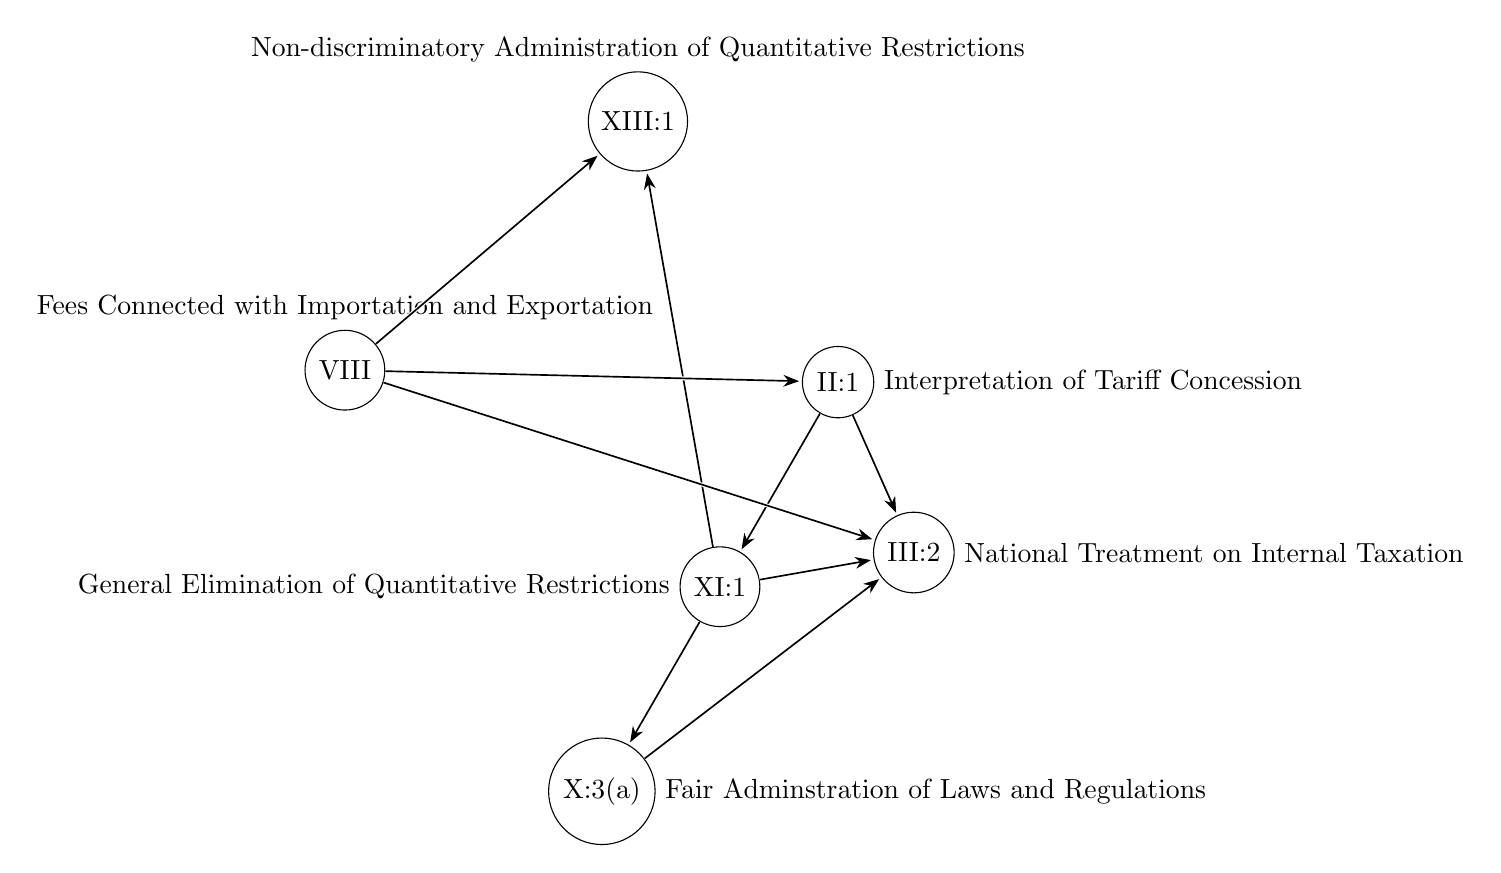
\begin{tikzpicture}[>={Stealth[color=black]},shorten >=1pt,node distance=2cm,on grid,initial/.style={}]
  \node[state, label=right:Interpretation of Tariff Concession] (T1) {II:1};
  \node[state, label=left:General Elimination of Quantitative Restrictions] at ([shift=({240:3 cm})]T1) (T4) {XI:1};
  \node[state, label=right:Fair Adminstration of Laws and Regulations] at ([shift=({240:3 cm})]T4) (T5) {X:3(a)};
  \node[state, label=above:Non-discriminatory Administration of Quantitative Restrictions] at ([shift=({100:6 cm})]T4) (T7) {XIII:1};
  \node[state, label=right:National Treatment on Internal Taxation] at ([shift=({10:2.5 cm})]T4) (T6) {III:2};
  \node[state, label=above:Fees Connected with Importation and Exportation] at ([shift=({150:5.5 cm})]T4) (T8) {VIII};

  \begin{scope}[every edge/.append style={->, double=black, draw=white}] % for directed edge, change "style={->, double=black, draw=white}]"
    \path (T1)
    edge   (T4)
    edge   (T6);
    \path (T4)
    edge   (T5)
    edge   (T6)
    edge   (T7);
    \path (T5)
    edge   (T6);
    \path (T8)
    edge   (T7)
    edge   (T1)
    edge   (T6);

  \end{scope}
\end{tikzpicture}

% to draw the node's border w/ color, refer to https://tex.stackexchange.com/questions/438412/how-to-add-border-to-a-node
    }
    \caption{{\bf Network of the Articles that Achieves \textit{Market Access}:}
        This figure demonstrates a network of articles of WTO agreements
        that cooperatively achieves the principle of \textit{Market Access} in the regulatory system of WTO.
        Tariff and Non-tariff barriers such as quantitative restriction, internal taxations
        and extra fees for crossing border can inhibit the chance of foreign goods to access the foreign market.
        Therefore, these articles tend to work together to ensure the \textit{Market Access} principle working properly.
        %(Directions and weights of network edges are omitted for brevity.)
    }
    \label{fig:market-aceess_directed}
  \end{figure}
  
% Figure \ref{fig:market-aceess_directed} shows a part of the fitted network $G^*$ that explains how
% the articles of WTO agreements are interconnected each other to acheive one of the main principles of 
% WTO, \textit{Market Access}. 
\textit{Market Access} 
refers to the guarantee of the conditions relating to the 
tariff or non-tariff measures 
for the entry of 
goods into the foreign market. For example, if 
a country set a limit on the quantity of imported goods, no foreign goods above that limit can get access to that market. Also, if a country set a high tariff rate for a imported goods to cross the border, 
it also prevents foreign goods from accessing to that market.
Therefore, \textit{Market Access} is the most basic but important principle of the WTO
because it directly represent the primary goal of the WTO, smoothing the world trade flow.

Three different types of measures - quantitative restriction, tariff and internal taxation or regulations - are recocgnized as 
three major types of measures that protectionistic country prefer to use. For example, a country can
discriminate imported and domestic product with internal regulation such as enforcing the specialized retail channel for the imported product as \textit{Korea - Beef} case as introduced in section \ref{subsec:design:dnn}.
This discrimination provide a unfair ground of competition between domestic and imported products and it can eventually exclude imported beef from the Korean beef market.
These three main types of measures that are relevant to the \textit{Market Access} is illustrated in Figure \ref{fig:market-aceess_directed}.
Article XI:1, II:1 and III correponds to the obligations that regulates quantitative restriction, tariff and internal taxation respectively.
Edges are colored in red if the mean of the two directed edge weights are greater than $10\%$. For example, $w^*(\text{II:1}, \text{III}) = 0.117$ and $w^*(\text{III}, \text{II:1}) = 0.122$ thus their simple mean is 11.95\% which is greater than 10\%.
This red triangle that is comprised of Article XI:1, II:1 and III shows that the fitted network $G^* = (V, E, W^*)$ captures the principle of \textit{Market Access} as a cluster of articles with large edge weights. Moreover, 
the fitted network $G^*$ also captures sub-articles that supports this \textit{Market Access} triangle. For example, I colored edges in blue if the mean of the two directed edge weights are greather than 5\% and less than 10\%.
The Article X:3(a) which prohibits a unfair adminstration of laws and regulations are connected to the Article XI:1 and III that are mostly 
deteriorates the principle of \textit{Market Access} by unfair adminstration of laws and regulations relating to the quantitative restriction 
and competitive relationship between imported and domestic products. Also, in a similar notion, Article VIII get connected to the Article II:1 because 
often the fees connected with the importation are charged with huge amount and can deteriorates the principle of \textit{Market Access} as well.

% Mean of directive edge weights between Article II:1, III and XI:1 are $0.289$, 



% having a sum of directive edge weights bigger than 0.15, which is about ten times bigger than that of  

% The three major articles of the WTO agreements 
% that regulates 


% \subsubsection{Market Access Principle Captured in a Reconstructed Network}
% % == THREE SUBSYSTEM == 
\begin{figure}[ht]
    \centering{
      % 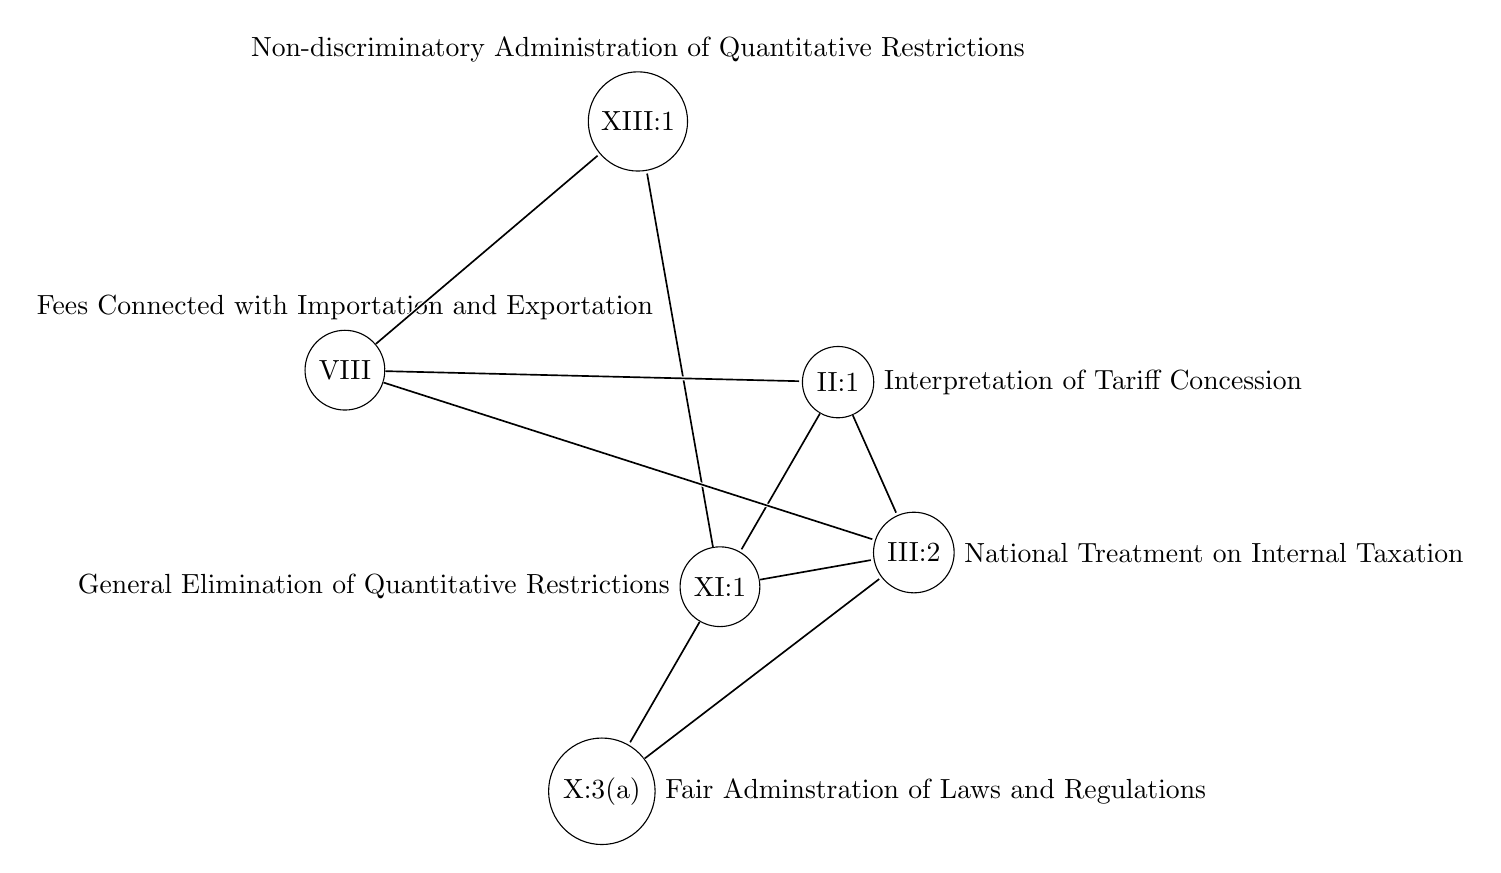
\begin{tikzpicture}[>={Stealth[color=black]},shorten >=1pt,node distance=2cm,on grid,initial/.style={}]
  \node[state, label=right:Interpretation of Tariff Concession] (T1) {II:1};
  \node[state, label=left:General Elimination of Quantitative Restrictions] at ([shift=({240:3 cm})]T1) (T4) {XI:1};
  \node[state, label=right:Fair Adminstration of Laws and Regulations] at ([shift=({240:3 cm})]T4) (T5) {X:3(a)};
  \node[state, label=above:Non-discriminatory Administration of Quantitative Restrictions] at ([shift=({100:6 cm})]T4) (T7) {XIII:1};
  \node[state, label=right:National Treatment on Internal Taxation] at ([shift=({10:2.5 cm})]T4) (T6) {III:2};
  \node[state, label=above:Fees Connected with Importation and Exportation] at ([shift=({150:5.5 cm})]T4) (T8) {VIII};

  \begin{scope}[every edge/.append style={-, double=black, draw=white}] % for directed edge, change "style={->, double=black, draw=white}]"
    \path (T1)
    edge   (T4)
    edge   (T6);
    \path (T4)
    edge   (T5)
    edge   (T6)
    edge   (T7);
    \path (T5)
    edge   (T6);
    \path (T8)
    edge   (T7)
    edge   (T1)
    edge   (T6);

  \end{scope}
\end{tikzpicture}

% to draw the node's border w/ color, refer to https://tex.stackexchange.com/questions/438412/how-to-add-border-to-a-node
      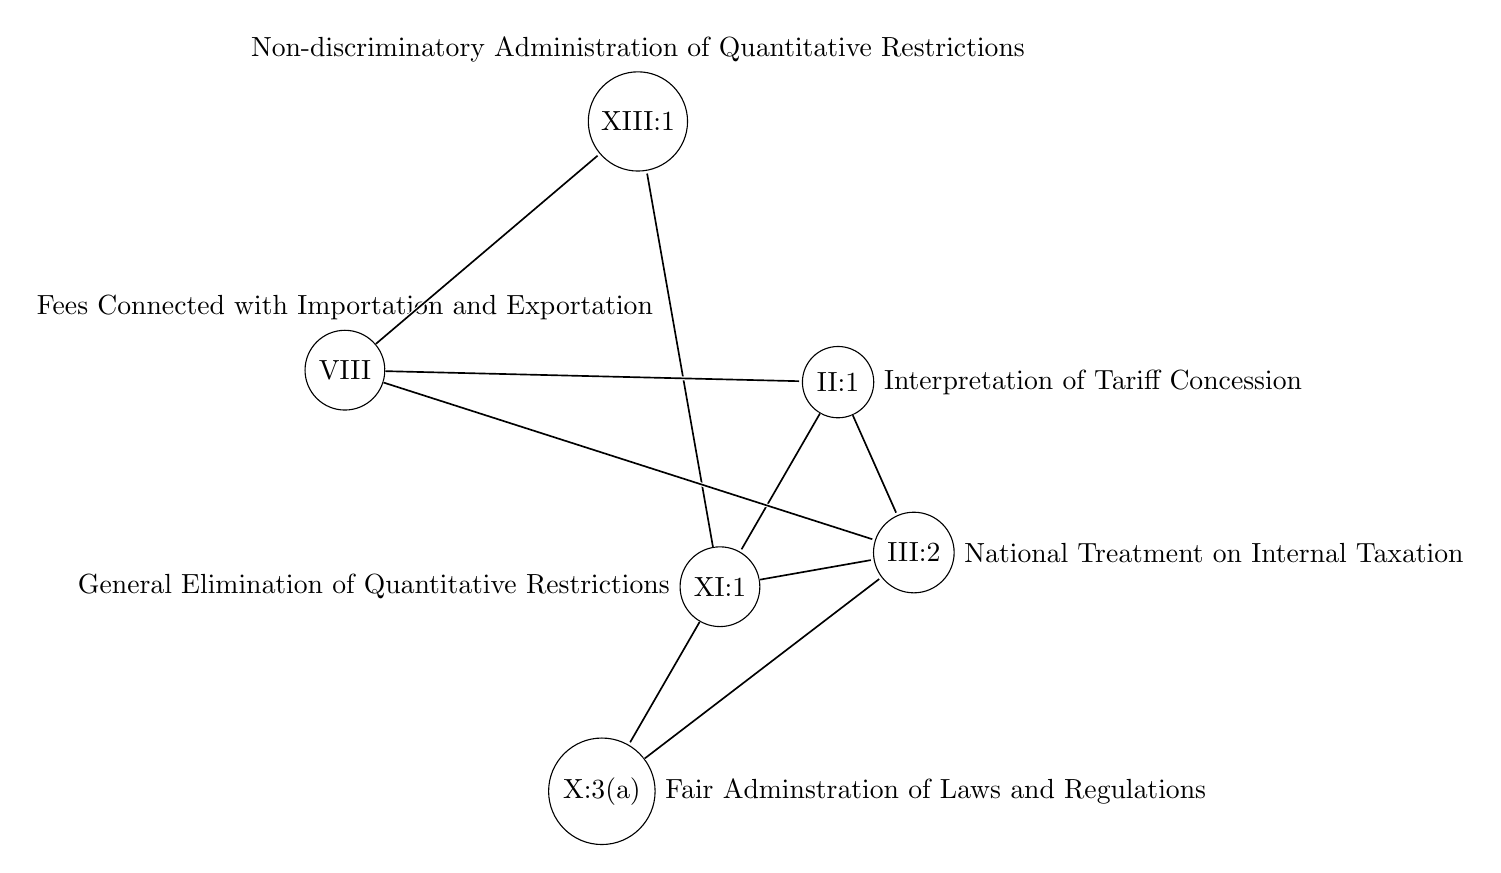
\begin{tikzpicture}[>={Stealth[color=black]},shorten >=1pt,node distance=2cm,on grid,initial/.style={}]
        \node[state, label=right:Interpretation of Tariff Concession] (T1) {II:1};
        \node[state, label=left:General Elimination of Quantitative Restrictions] at ([shift=({240:3cm})]T1) (T4) {XI:1};
        \node[state, label=right:Fair Adminstration of Laws and Regulations] at ([shift=({240:3 cm})]T4) (T5) {X:3(a)};
        \node[state, label=above:Non-discriminatory Administration of Quantitative Restrictions] at ([shift=({100:6 cm})]T4) (T7) {XIII:1};
        \node[state, label=right:National Treatment on Internal Taxation] at ([shift=({10:2.5 cm})]T4) (T6) {III:2};
        \node[state, label=above:Fees Connected with Importation and Exportation] at ([shift=({150:5.5 cm})]T4) (T8) {VIII};
        
        \begin{scope}[every edge/.append style={-, double=black, draw=white}] % for directed edge, change "style={->, double=black, draw=white}]"
          \path (T1)
          edge   (T4)
          edge   (T6);
          \path (T4)
          edge   (T5)
          edge   (T6)
          edge   (T7);
          \path (T5)
          edge   (T6);
          \path (T8)
          edge   (T7)
          edge   (T1)
          edge   (T6);
        \end{scope}

        % \draw[line width=0.1pt,red,double=red,double distance=1pt] (T6) -- (T4); %III:2, XI:1
        % \draw[line width=0.1pt,magenta,double=black,double distance=1pt] (T1) -- (T6); % II:1 III:2 
        % \draw[line width=1pt,black,double=black,double distance=1pt] (T1) -- (T4); % II:1 III:2

      \end{tikzpicture}
    }
    \caption{Market Access}
    \label{fig:market-aceess}
  \end{figure}
  

  % XI:1 <-> III:2 :: 0.232
  % II:1 <-> III:2 :: 0.2385
  ------
  % II:1 <-> XI:1 :: 0.19
  % X:3(a) <-> III:2 :: 0.196
  % X:3(a) <-> X:3(a) :: 0.184
  ------
  % VIII <-> II:1 :: 0.167
  % XI:1 <-> XIII:1 :: 0.169
  -----
  % VIII <-> III:2 :: 0.138
  % VIII <-> II:1 :: 0.138
  ----



\section{Conclusion}
% This paper shows how WTO works.

% \begin{itemize}
%   \item Implicaiton of thie method in general.
%   \item Address the imbalance of legal capacity between developed/ing countries
% \end{itemize}

\clearpage \bibliography{bibtemplate}

\clearpage
\begin{appendices}
\section{}
\label{sec:appendix}
% \subsection{Table of Contents of the Panel Report}
% \begin{figure}[h]
    \centering
    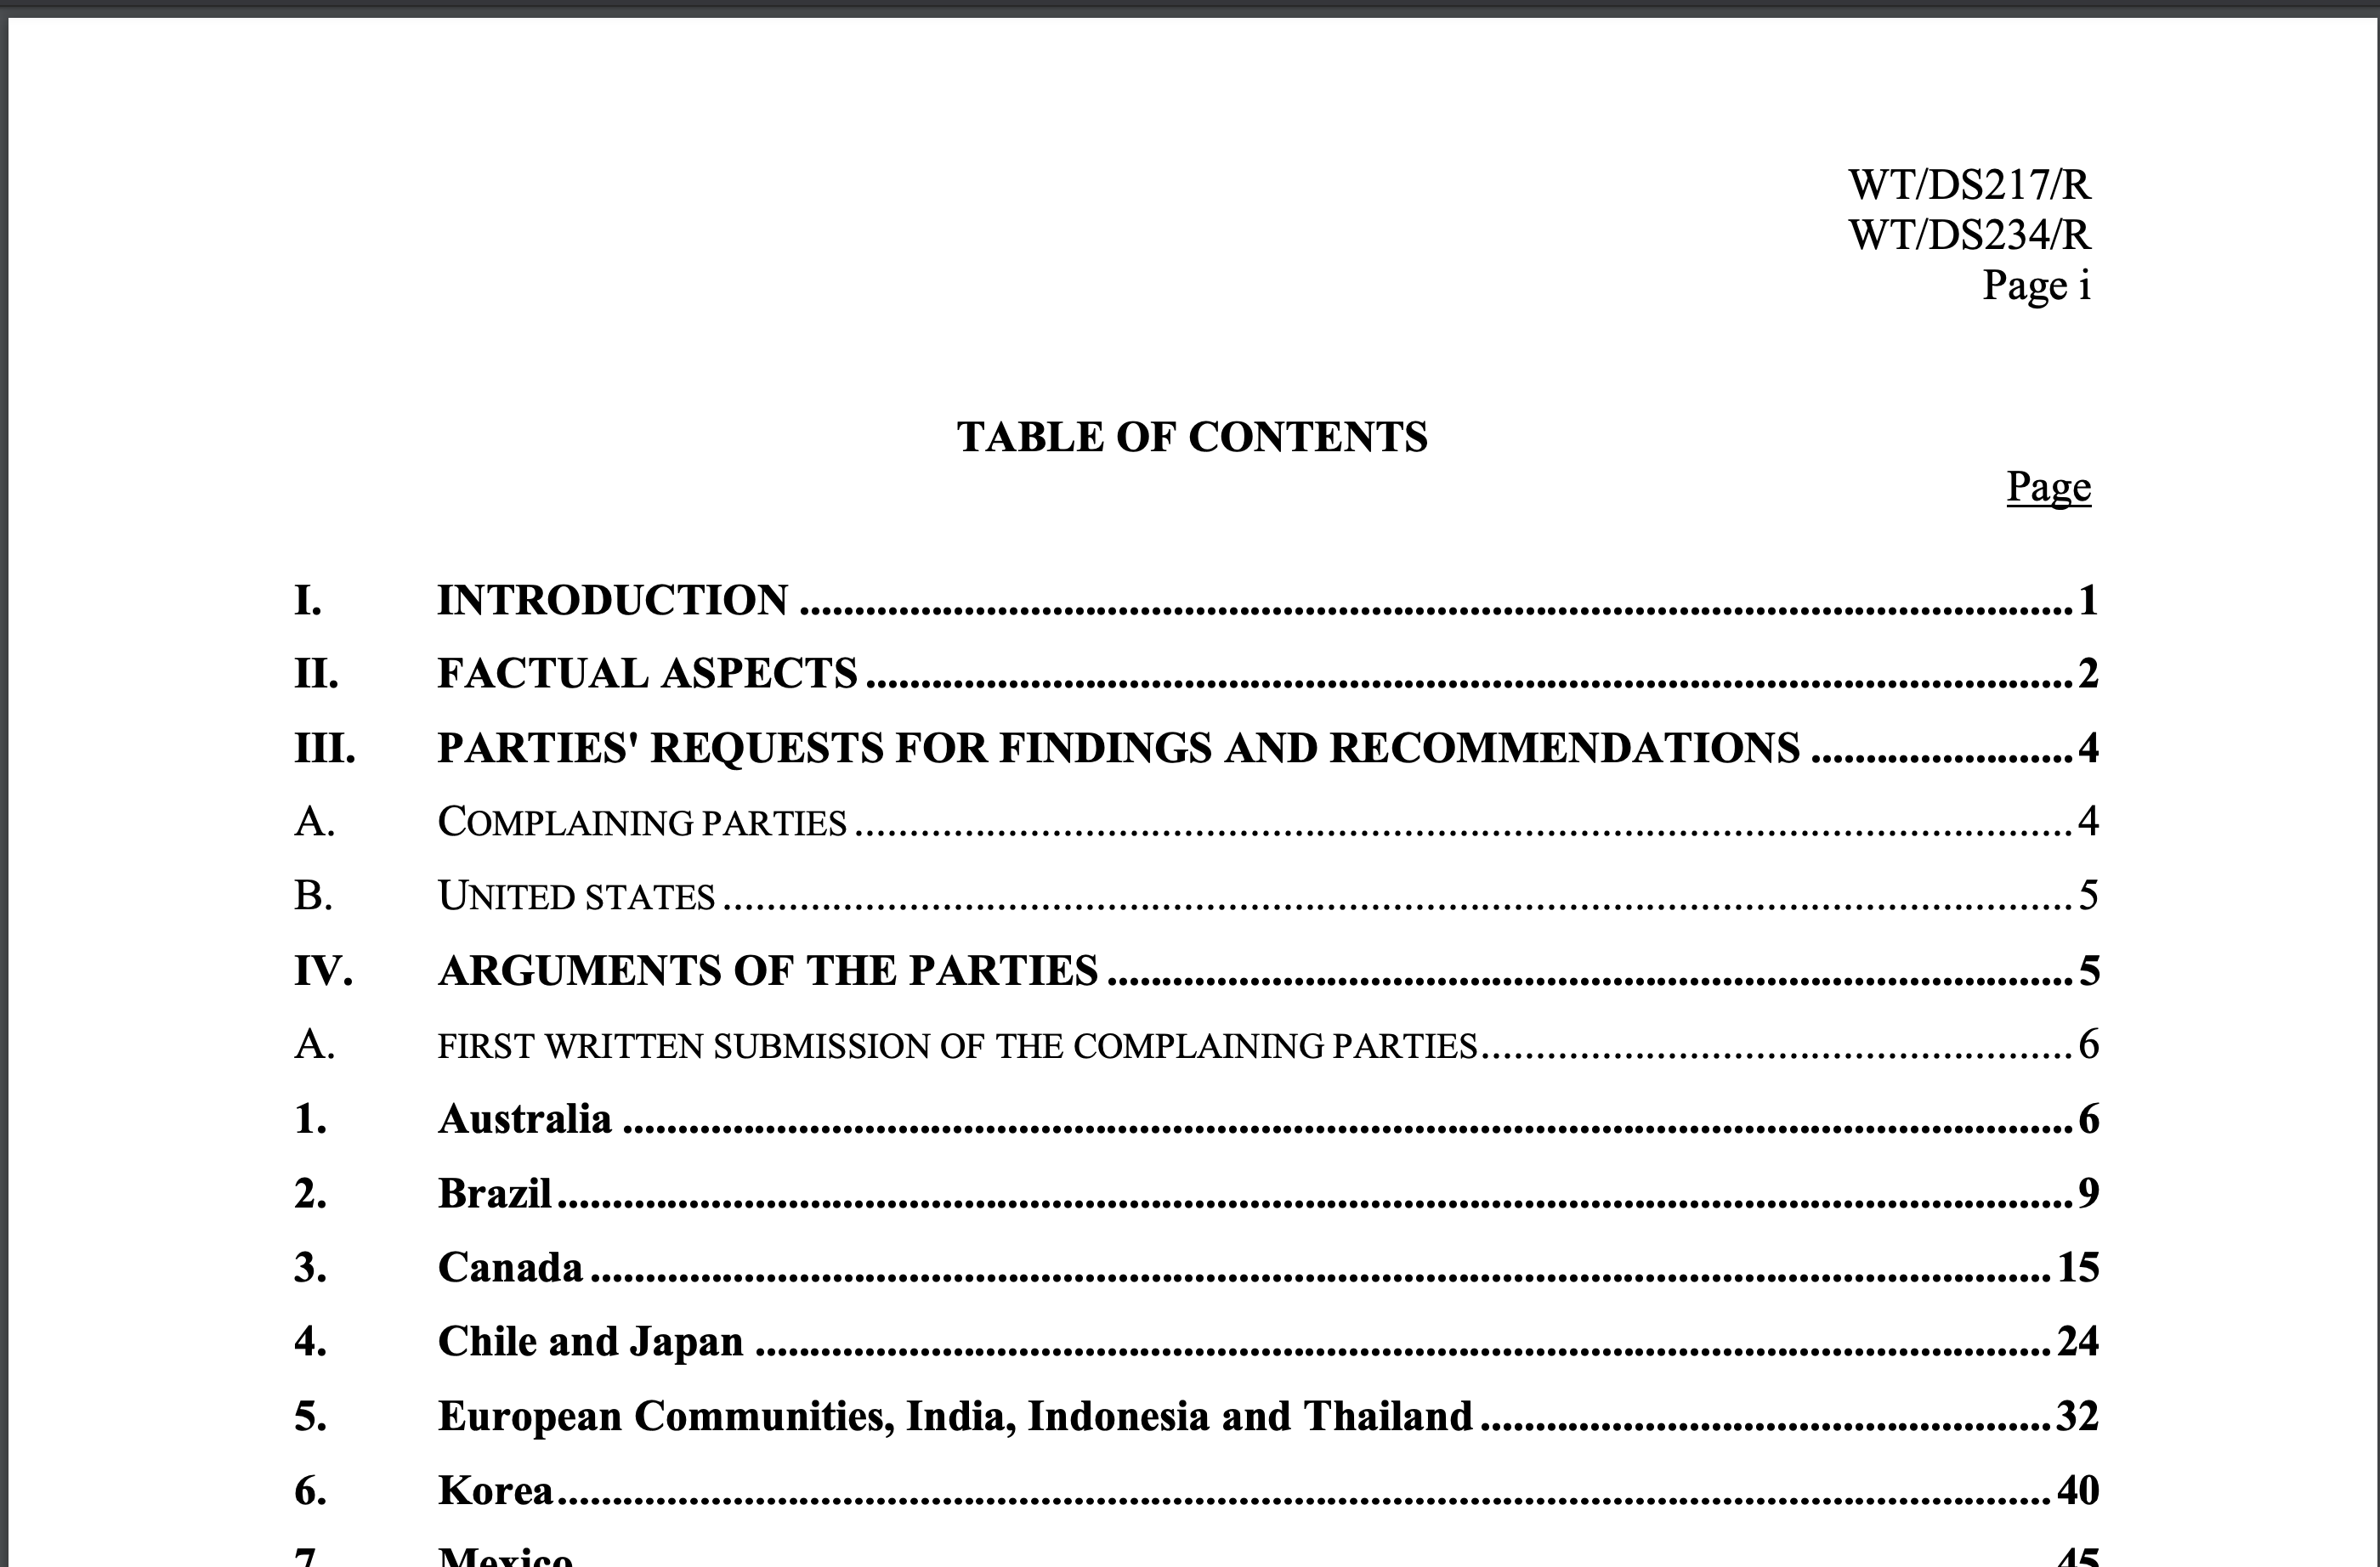
\includegraphics[scale=0.28]{Data/pngs/panel_report_toc.png}
    \caption{
        {\bf Table of Contents of Panel Report: }Panel provides 
        factual aspect in the panel report with its page location.
        }
    \label{fig:panel-report-toc}
\end{figure}
% \begin{center}
%     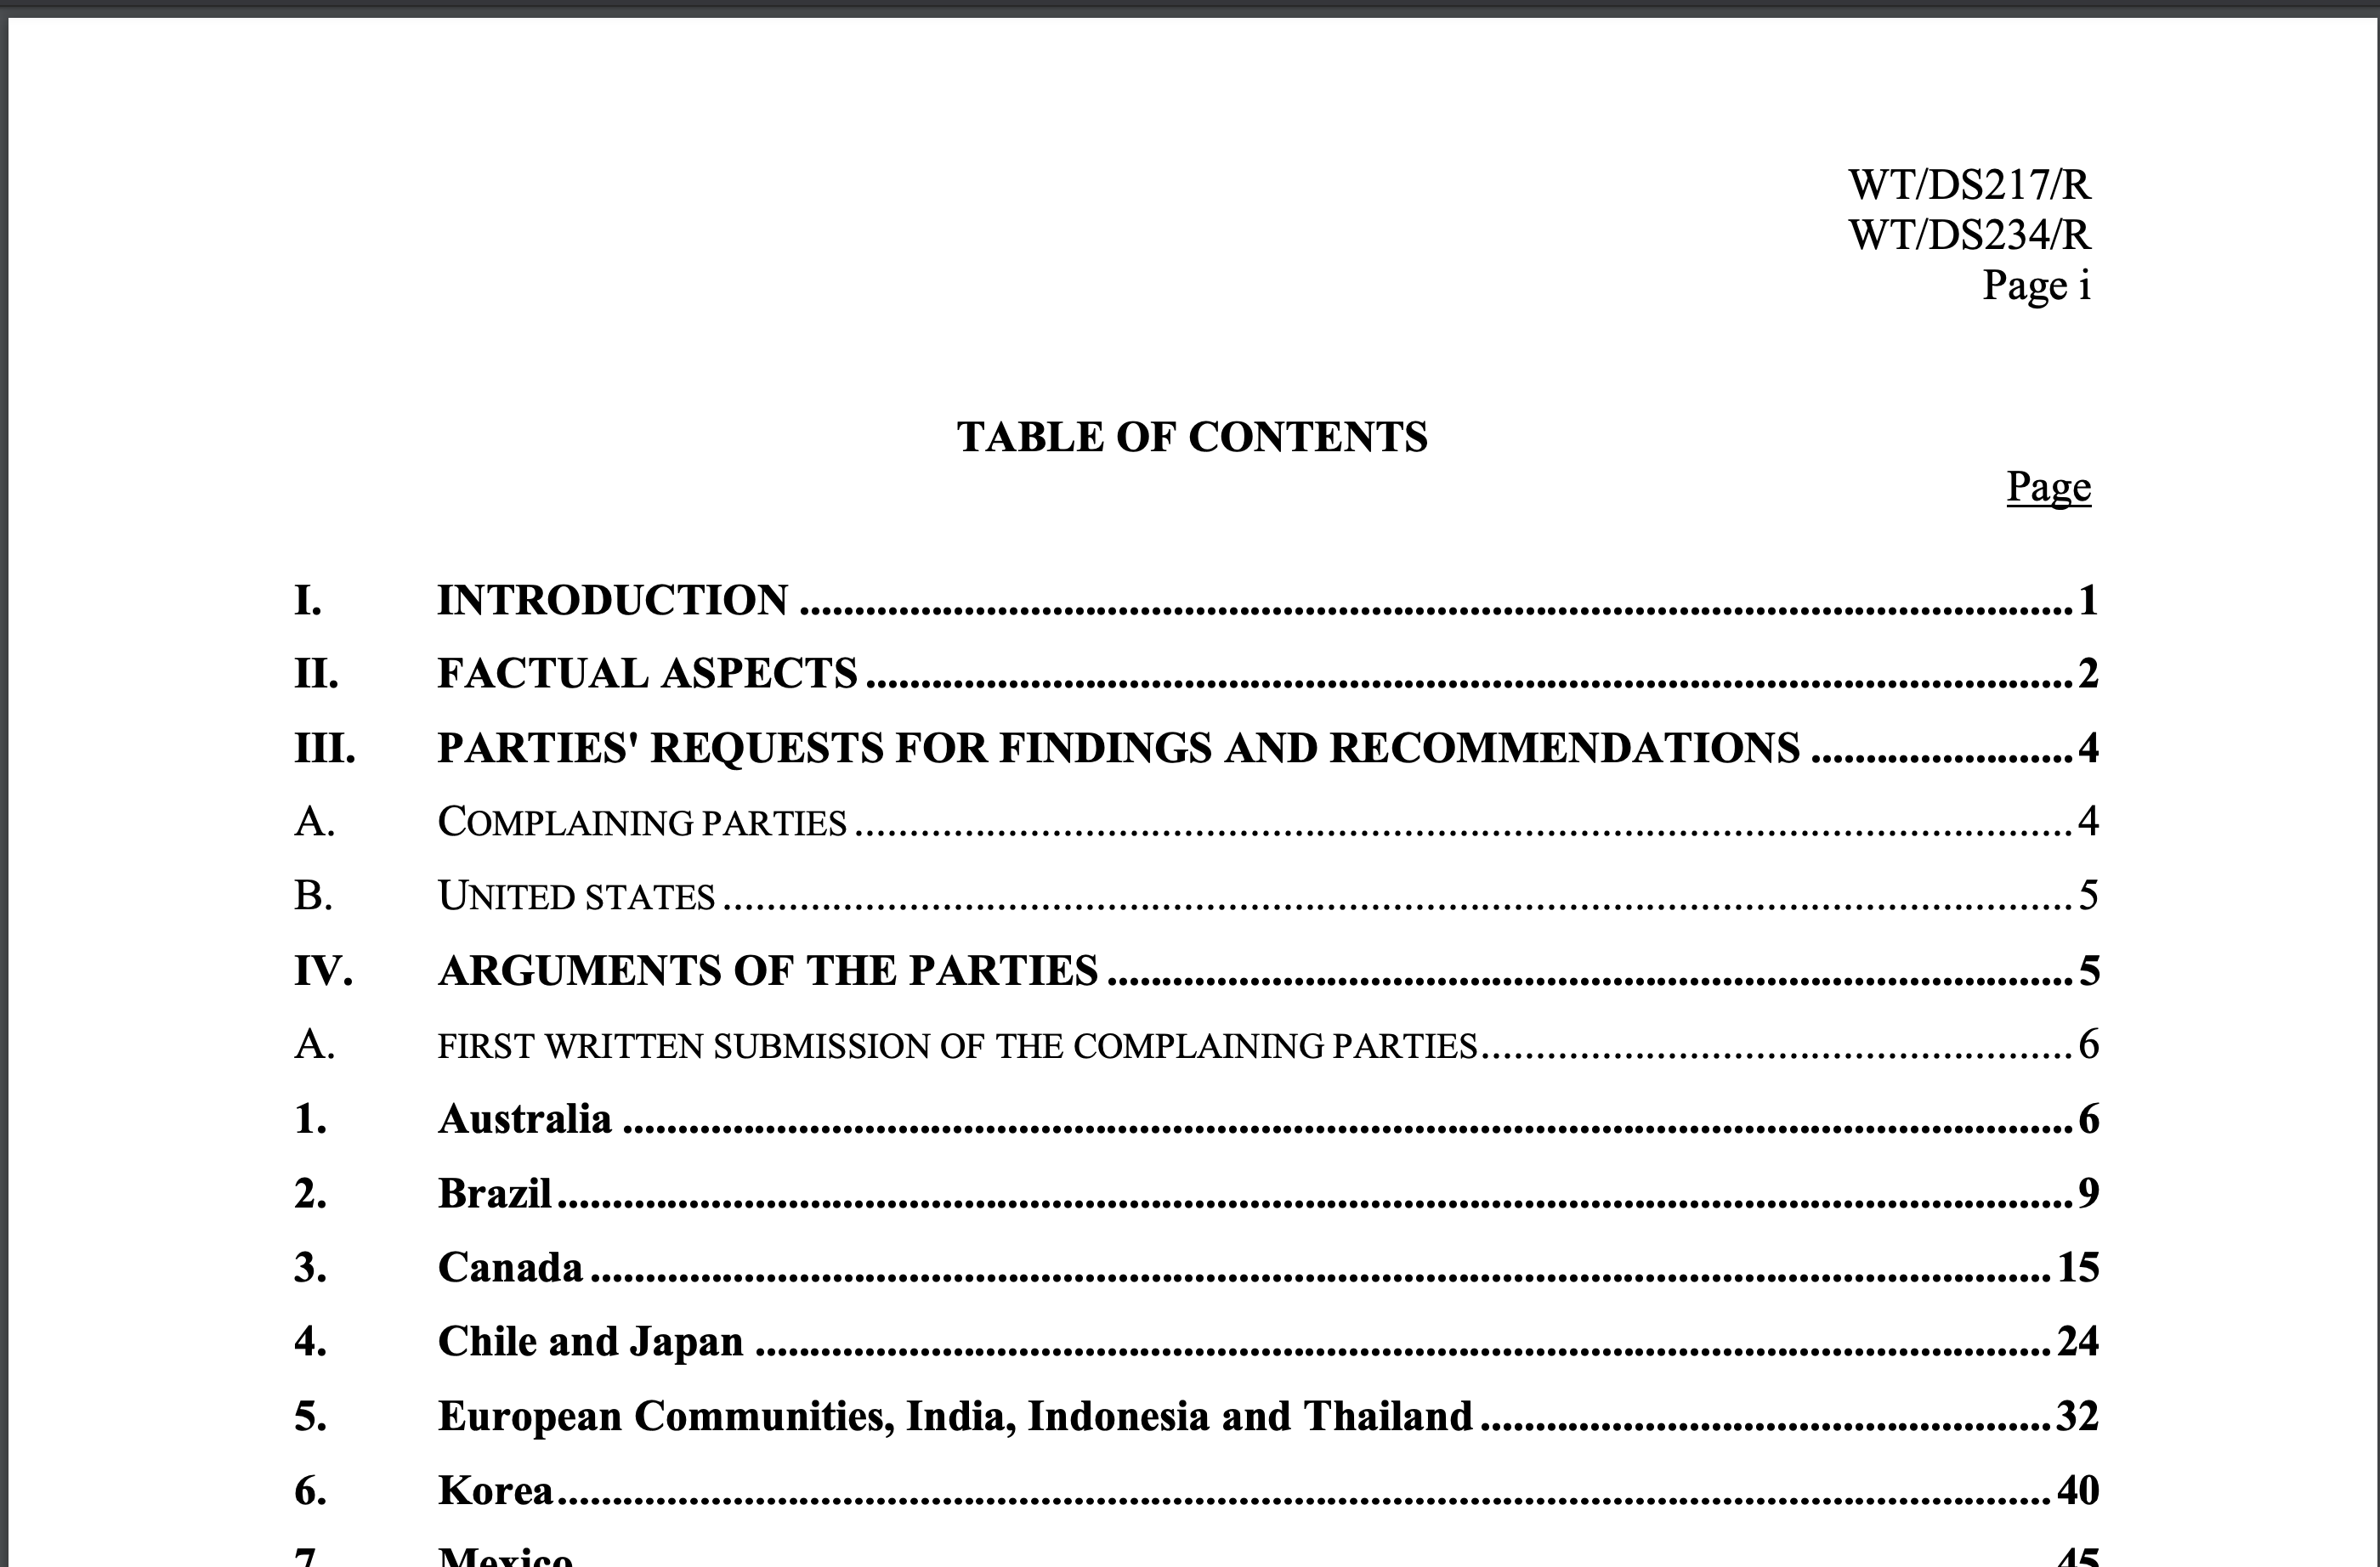
\includegraphics[scale=0.3]{Data/pngs/panel_report_toc.png}
% \end{center}



\subsection{Factual Aspect Example}
\label{sub:factual-aspect-example}
Excerpt below is from the panel report for the 
\textit{US - Offset Act (Byrd Amendment)}
\footnote{Panel Report, nited States — Continued Dumping and Subsidy Offset Act of 2000, WTO Doc. WT/DS217/R (adopted Jan. 27, 2003).} case.\\

\begin{tcolorbox}[breakable]
\noindent{\bf II. FACTUAL ASPECTS}\\\\
2.1 \quad This dispute concerns the Continued Dumping and Subsidy Offset Act of 2000 (the
“CDSOA” or the “Offset Act”), which was enacted on 28 October 2000 as part of the Agriculture,
Rural Development, Food and Drug Administration and Related Agencies Appropriations Act, 2001.1
The CDSOA amends Title VII of the Tariff Act of 1930 by adding a new section 754 entitled
Continued Dumping and Subsidy Offset. Regulations prescribing administrative procedures under the
Act were brought into effect on September 21, 2001.\\

\noindent2.2 \quad The CDSOA provides that :

\blockquote{
    Duties assessed pursuant to a countervailing duty order, an anti-dumping duty order,
    or a finding under the Antidumping Act of 1921 shall be distributed on an annual
    basis under this section to the affected domestic producers for qualifying
    expenditures. Such distribution shall be known as “the continued dumping and
    subsidy offset”.
    }
\\\\
\noindent2.3 \quad The term “affected domestic producers” means :

\blockquote{
    a manufacturer, producer, farmer, rancher, or worker representative (including
associations of such persons) that – \\\\
        (A) was a petitioner or interested party in support of the petition with respect
to which an anti-dumping duty order, a finding under the Antidumping Act of 1921,
or a countervailing duty order has been entered, and \\\\
\quad \quad (B) remains in operation. \\\\
Companies, business, or persons that have ceased the production of the product
covered by the order or finding or who have been acquired by a company or business
that is related to a company that opposed the investigation shall not be an affected
domestic producer.
}
\\\\
\noindent 2.4 \quad In turn, the term “qualifying expenditure” is defined by the CDSOA as “expenditure[s]
incurred after the issuance of the anti-dumping duty finding or order or countervailing duty order in
any of the following categories:
\blockquote{
(A) Manufacturing facilities.\\
(B) Equipment.\\
(C) Research and development.\\
(D) Personnel training.\\
(E) Acquisition of technology.\\
(F) Health care benefits to employees paid for by the employer.\\
(G) Pension benefits to employees paid for by the employer.\\
(H) Environmental equipment, training or technology.\\
(I) Acquisition of raw materials and other inputs.\\
(J) Working capital or other funds needed to maintain production.”
}
\\\\
\noindent 2.5 \quad The CDSOA provides that the Commissioner of Customs shall establish in the Treasury of
the United States a special account with respect to each order or finding8
 and deposit into such
account all the duties assessed under that Order.9
 The Commissioner of Customs shall distribute all
funds (including all interest earned on the funds) from the assessed duties received in the preceding
fiscal year to affected domestic producers based on a certification by the affected domestic producer
that he is eligible to receive the distribution and desires to receive a distribution for qualifying
expenditures incurred since the issuance of the order or finding.10 Funds deposited in each special
account during each fiscal year are to be distributed no later than 60 days after the beginning of the
following fiscal year.11 The CDSOA and regulations prescribe that (1) if the total amount of the
certified net claims filed by affected domestic producers does not exceed the amount of the offset
available, the certified net claim for each affected domestic producer will be paid in full, and (2) if the
certified net claims exceed the amount available, the offset will be made on a pro rata basis based on
each affected domestic producer’s total certified claim.\\

\noindent 2.6 \quad Special accounts are to be terminated after “(A) the order or finding with respect to which the
account was established has terminated; (B) all entries relating to the order or finding are liquidated
and duties assessed collected; (C) the Commissioner has provided notice and a final opportunity to
obtain distribution pursuant to subsection (c); and (D) 90 days has elapsed from the date of the notice
described in subparagraph (C).” All amounts that remain unclaimed in the Account are to be
permanently deposited into the general fund in the US Treasury.12\\

\noindent 2.7 \quad The CDSOA applies with respect to all anti-dumping and countervailing duty assessments
made on or after 1 October 200013 pursuant to an anti-dumping order or a countervailing order or a
finding under the Antidumping Act of 1921 in effect on 1 January 1999 or issued thereafter.

\end{tcolorbox}

% \subsection{Content of Legal Article Example}


\subsection{Collected Cited Articles for 143 WTO DSB Cases}
DS refers to \textit{Dispute Settelement} and this notation is officially adopted by WTO DSB.\\
WTO DSB identifies each dispute with a unique number for each case such as DS2 and DS18.
\label{sub:cited-articles-table}

\begin{xltabular}{\linewidth}{ l | X }
    % \caption{Description of Variables used in this Study}
    % \label{table: vardescription}
    \hline 

    \textbf{\normalsize DS} & \textbf{\normalsize Articles Cited}  \\
    \endfirsthead
    \hline \hline

    \textbf{DS2} & I, II:1(b) \\ \hline

    \textbf{DS3} & I, II:1(b) \\ \hline

    \textbf{DS2} & I, II:1(b) \\ \hline

    \textbf{DS3} & I, II:1(b) \\ \hline

    \textbf{DS2} & I, II:1(b) \\ \hline

    \textbf{DS3} & I, II:1(b) \\ \hline

    \textbf{DS2} & I, II:1(b) \\ \hline

    \textbf{DS3} & I, II:1(b) \\ \hline

    \textbf{DS2} & I, II:1(b) \\ \hline

    \textbf{DS3} & I, II:1(b) \\ \hline

    \textbf{DS2} & I, II:1(b) \\ \hline

    \textbf{DS3} & I, II:1(b) \\ \hline

    \textbf{DS2} & I, II:1(b) \\ \hline

    \textbf{DS3} & I, II:1(b) \\ \hline

    \textbf{DS2} & I, II:1(b) \\ \hline

    \textbf{DS3} & I, II:1(b) \\ \hline

    \textbf{DS2} & I, II:1(b) \\ \hline

    \textbf{DS3} & I, II:1(b) \\ \hline

    \textbf{DS2} & I, II:1(b) \\ \hline

    \textbf{DS3} & I, II:1(b) \\ \hline

    \textbf{DS2} & I, II:1(b) \\ \hline

    \textbf{DS3} & I, II:1(b) \\ \hline

    \textbf{DS2} & I, II:1(b) \\ \hline

    \textbf{DS3} & I, II:1(b) \\ \hline

    \textbf{DS2} & I, II:1(b) \\ \hline

    \textbf{DS3} & I, II:1(b) \\ \hline

    \textbf{DS2} & I, II:1(b) \\ \hline

    \textbf{DS3} & I, II:1(b) \\ \hline

    \textbf{DS2} & I, II:1(b) \\ \hline

    \textbf{DS3} & I, II:1(b) \\ \hline

    \textbf{DS2} & I, II:1(b) \\ \hline

    \textbf{DS3} & I, II:1(b) \\ \hline

    \textbf{DS2} & I, II:1(b) \\ \hline

    \textbf{DS3} & I, II:1(b) \\ \hline

    \textbf{DS2} & I, II:1(b) \\ \hline

    \textbf{DS3} & I, II:1(b) \\ \hline

    \textbf{DS2} & I, II:1(b) \\ \hline

    \textbf{DS3} & I, II:1(b) \\ \hline

    \textbf{DS2} & I, II:1(b) \\ \hline

    \textbf{DS3} & I, II:1(b) \\ \hline

    \textbf{DS2} & I, II:1(b) \\ \hline

    \textbf{DS3} & I, II:1(b) \\ \hline

    \textbf{DS2} & I, II:1(b) \\ \hline

    \textbf{DS3} & I, II:1(b) \\ \hline

    \textbf{DS2} & I, II:1(b) \\ \hline

    \textbf{DS3} & I, II:1(b) \\ \hline

    \textbf{DS2} & I, II:1(b) \\ \hline

    \textbf{DS3} & I, II:1(b) \\ \hline

    \textbf{DS2} & I, II:1(b) \\ \hline

    \textbf{DS3} & I, II:1(b) \\ \hline

    \textbf{DS2} & I, II:1(b) \\ \hline

    \textbf{DS3} & I, II:1(b) \\ \hline

    \textbf{DS2} & I, II:1(b) \\ \hline

    \textbf{DS3} & I, II:1(b) \\ \hline

    \textbf{DS2} & I, II:1(b) \\ \hline

    \textbf{DS3} & I, II:1(b) \\ \hline

    \textbf{DS2} & I, II:1(b) \\ \hline

    \textbf{DS3} & I, II:1(b) \\ \hline

    \textbf{DS2} & I, II:1(b) \\ \hline

    \textbf{DS3} & I, II:1(b) \\ \hline

    \textbf{DS2} & I, II:1(b) \\ \hline

    \textbf{DS3} & I, II:1(b) \\ \hline

    \textbf{DS2} & I, II:1(b) \\ \hline

    \textbf{DS3} & I, II:1(b) \\ \hline

    \textbf{DS2} & I, II:1(b) \\ \hline

    \textbf{DS3} & I, II:1(b) \\ \hline

    \textbf{DS2} & I, II:1(b) \\ \hline

    \textbf{DS3} & I, II:1(b) \\ \hline

    \textbf{DS2} & I, II:1(b) \\ \hline

    \textbf{DS3} & I, II:1(b) \\ \hline

    \textbf{DS2} & I, II:1(b) \\ \hline

    \textbf{DS3} & I, II:1(b) \\ \hline

    \textbf{DS2} & I, II:1(b) \\ \hline

    \textbf{DS3} & I, II:1(b) \\ \hline

    \textbf{DS2} & I, II:1(b) \\ \hline

    \textbf{DS3} & I, II:1(b) \\ \hline

    \textbf{DS2} & I, II:1(b) \\ \hline

    \textbf{DS3} & I, II:1(b) \\ \hline

    \textbf{DS2} & I, II:1(b) \\ \hline

    \textbf{DS3} & I, II:1(b) \\ \hline

    \textbf{DS2} & I, II:1(b) \\ \hline

    \textbf{DS3} & I, II:1(b) \\ \hline

    \textbf{DS2} & I, II:1(b) \\ \hline

    \textbf{DS3} & I, II:1(b) \\ \hline

    \textbf{DS2} & I, II:1(b) \\ \hline

    \textbf{DS3} & I, II:1(b) \\ \hline

    \textbf{DS2} & I, II:1(b) \\ \hline

    \textbf{DS3} & I, II:1(b) \\ \hline

    \textbf{DS2} & I, II:1(b) \\ \hline

    \textbf{DS3} & I, II:1(b) \\ \hline

    \textbf{DS2} & I, II:1(b) \\ \hline

    \textbf{DS3} & I, II:1(b) \\ \hline

    \textbf{DS2} & I, II:1(b) \\ \hline

    \textbf{DS3} & I, II:1(b) \\ \hline

    \textbf{DS2} & I, II:1(b) \\ \hline

    \textbf{DS3} & I, II:1(b) \\ \hline

    \textbf{DS2} & I, II:1(b) \\ \hline

    \textbf{DS3} & I, II:1(b) \\ \hline

    \textbf{DS2} & I, II:1(b) \\ \hline

    \textbf{DS3} & I, II:1(b) \\ \hline

    \textbf{DS2} & I, II:1(b) \\ \hline

    \textbf{DS3} & I, II:1(b) \\ \hline

    \textbf{DS2} & I, II:1(b) \\ \hline

    \textbf{DS3} & I, II:1(b) \\ \hline

    \textbf{DS2} & I, II:1(b) \\ \hline

    \textbf{DS3} & I, II:1(b) \\ \hline

    \textbf{DS2} & I, II:1(b) \\ \hline

    \textbf{DS3} & I, II:1(b) \\ \hline

    \textbf{DS2} & I, II:1(b) \\ \hline

    \textbf{DS3} & I, II:1(b) \\ \hline

    \textbf{DS2} & I, II:1(b) \\ \hline

    \textbf{DS3} & I, II:1(b) \\ \hline

    \textbf{DS2} & I, II:1(b) \\ \hline

    \textbf{DS3} & I, II:1(b) \\ \hline

    \textbf{DS2} & I, II:1(b) \\ \hline

    \textbf{DS3} & I, II:1(b) \\ \hline

    \textbf{DS2} & I, II:1(b) \\ \hline

    \textbf{DS3} & I, II:1(b) \\ \hline

    \textbf{DS2} & I, II:1(b) \\ \hline

    \textbf{DS3} & I, II:1(b) \\ \hline

    \textbf{DS2} & I, II:1(b) \\ \hline

    \textbf{DS3} & I, II:1(b) \\ \hline

    \textbf{DS2} & I, II:1(b) \\ \hline

    \textbf{DS3} & I, II:1(b) \\ \hline

    \textbf{DS2} & I, II:1(b) \\ \hline

    \textbf{DS3} & I, II:1(b) \\ \hline

    \textbf{DS2} & I, II:1(b) \\ \hline

    \textbf{DS3} & I, II:1(b) \\ \hline

    \textbf{DS2} & I, II:1(b) \\ \hline

    \textbf{DS3} & I, II:1(b) \\ \hline

    \textbf{DS2} & I, II:1(b) \\ \hline

    \textbf{DS3} & I, II:1(b) \\ \hline

    \textbf{DS2} & I, II:1(b) \\ \hline

    \textbf{DS3} & I, II:1(b) \\ \hline

    \textbf{DS2} & I, II:1(b) \\ \hline

    \textbf{DS3} & I, II:1(b) \\ \hline

    \textbf{DS2} & I, II:1(b) \\ \hline

    \textbf{DS3} & I, II:1(b) \\ \hline

    \textbf{DS2} & I, II:1(b) \\ \hline

    \textbf{DS3} & I, II:1(b) \\ \hline

    \textbf{DS2} & I, II:1(b) \\ \hline

    \textbf{DS3} & I, II:1(b) \\ \hline

    \textbf{DS2} & I, II:1(b) \\ \hline \hline

\end{xltabular}

\subsection{Technical Details}
\label{sub:technicial-details}

% == HEATMAP MATRIX == 
\begin{figure}[!tbp]
    \begin{subfigure}[b]{0.49\textwidth}
      \centering{
        \resizebox{\textwidth*\real{\heatmap}}{\textwidth*\real{\heatmap} * \real{1.7889}}{% This file was created by tikzplotlib v0.9.4.
\begin{tikzpicture}

\begin{axis}[
hide x axis,
hide y axis,
tick align=outside,
tick pos=left,
x grid style={white!69.0196078431373!black},
xmin=0, xmax=80,
xtick style={color=black},
y grid style={white!69.0196078431373!black},
ymin=0, ymax=143,
ytick style={color=black}
]
\addplot graphics [includegraphics cmd=\pgfimage,xmin=0, xmax=80, ymin=0, ymax=143] {co-citation-004.png};
\end{axis}

\end{tikzpicture}
}
        \caption{Co-citation}
        \label{sparse_matrix}
      }
    \end{subfigure}
    \hfill
    \begin{subfigure}[b]{0.49\textwidth}
      \centering{
        \resizebox{\textwidth*\real{\heatmap}}{\textwidth*\real{\heatmap} * \real{1.7889}}{% This file was created by tikzplotlib v0.9.4.
\begin{tikzpicture}

\begin{axis}[
hide x axis,
hide y axis,
tick align=outside,
tick pos=left,
x grid style={white!69.0196078431373!black},
xmin=0, xmax=80,
xtick style={color=black},
y grid style={white!69.0196078431373!black},
ymin=0, ymax=143,
ytick style={color=black}
]
\addplot graphics [includegraphics cmd=\pgfimage,xmin=0, xmax=80, ymin=0, ymax=143] {pred_only.png};
\end{axis}

\end{tikzpicture}
}
        \caption{Prediction}
        \label{predidction_matrix}
      }
    \end{subfigure}
    \caption{{\bf Co-citation \& Prediction}}
    \label{sparse_dense}
  \end{figure}
  

% % This file was created by tikzplotlib v0.9.4.
\begin{tikzpicture}

\begin{axis}[
tick align=outside,
tick pos=left,
title={coo},
x grid style={white!69.0196078431373!black},
xmin=0, xmax=58,
xtick style={color=black},
y grid style={white!69.0196078431373!black},
ymin=0, ymax=58,
ytick style={color=black}
]
\addplot graphics [includegraphics cmd=\pgfimage,xmin=0, xmax=58, ymin=0, ymax=58] {coo-001.png};
\end{axis}

\end{tikzpicture}

\end{appendices}
\end{document}